\documentclass[10pt,landscape,twocolumn]{article}

\usepackage[cm]{fullpage}
\usepackage[utf8]{inputenc}
\usepackage[ngerman,english]{babel}
\usepackage{amsmath,amssymb,amsthm}
\usepackage[pdftex]{graphicx}
% \usepackage{appendix}
% \usepackage{color}
% \usepackage{colortbl} % for colored hlines in chapter pagestyle
\usepackage{url}
% \usepackage{scrpage2}
% \usepackage{booktabs} % publication quality tables for LaTeX
\usepackage{algorithm}
% \usepackage{scrhack} % removes warning from KOMA
% \usepackage{helvet} % sets sans-serif font
% \usepackage{algpseudocode}
% \usepackage{csquotes}
\usepackage{pdfpages}

% pdf hyperlinks
\usepackage[pdftex,
		bookmarks,
		bookmarksopen=true,
		bookmarksnumbered=true,
		pdfauthor={Yeara Kozlov},
		pdftitle={},
		colorlinks,
		linkcolor=black,
		citecolor=black,
		filecolor=black,
		urlcolor=black,
		anchorcolor=black,
		menucolor=black,
		breaklinks=true,
		pageanchor=true,
		plainpages=false,
		pdfpagelabels=true]{hyperref}



\DeclareOldFontCommand{\bf}{\normalfont\bfseries}{\mathbf}

\usepackage{caption} 

\usepackage[slantedGreek]{mathpazo}

\usepackage{named}
\bibliographystyle{named}

\setlength\parindent{0pt}

%!TEX root = thesis.tex
\definecolor{ChapterColor}{cmyk}{0.9827,0.8405,0.0333,0.005}
\definecolor{TitleColor}{cmyk}{0.9827,0.8405,0.0333,0.005}

% Terminates current page and paragraph, makes sure next page starts on
% an odd-number, and generates a completely blank page, without page markers,
% if necessary.
\newcommand{\clearemptydoublepage}{\newpage{\pagestyle{empty}\cleardoublepage}}


\newcommand{\Ds}{\mathbf{D_s}} 
\newcommand{\F}{\mathbf{F}} 
\newcommand{\X}{\mathbf{X}} 
\newcommand{\x}{\mathbf{x}} 
\newcommand{\Dm}{\mathbf{D_s}}


\newcommand{\comment}[1]{}
\newcommand{\figref}[1]{Fig.~\ref{#1}}
\newcommand{\tabref}[1]{Table~\ref{#1}}
\newcommand{\eqnref}[1]{Eq.~\ref{#1}}
\newcommand{\secref}[1]{Section~\ref{#1}}
\newcommand{\chapref}[1]{Chapter~\ref{#1}}
\newcommand{\appref}[1]{Appendix~\ref{#1}}
\newcommand{\stepref}[1]{Step~\ref{#1}}
\newcommand{\algoref}[1]{Algorithm~\ref{#1}} %conflicts with algo package


\DeclareMathOperator*{\argmin}{argmin}
\DeclareMathOperator*{\argmax}{argmax}
\DeclareMathOperator*{\median}{median}
\DeclareMathOperator*{\Tr}{tr}

\definecolor{yearacolor}{RGB}{255,0,0}
\newcommand\yk[1] {\emph{\textcolor{yearacolor}{YK: #1}}}
\newcommand\yeara[1] {\emph{\textcolor{yearacolor}{YK: #1}}}

\newcommand\todo[1] {\emph{\textcolor{red}{#1}}}

\newcommand{\figtext}[1]{{\footnotesize #1}}

\newcommand{\bx}{\mathbf{x}}
\newcommand{\ba}{\mathbf{a}}
% \newcommand{\bf}{\mathbf{f}}
\newcommand{\bX}{\mathbf{X}}
\newcommand{\bE}{\mathbf{E}}
\newcommand{\bLF}{\mathbf{F}}
\newcommand{\bff}{\mathbf{f}}
\newcommand{\bM}{\mathbf{M}}

\graphicspath{{figures/}}

\begin{document}

\selectlanguage{english}

\title{Deep Learning Revision Notes}
\author{Yeara Kozlov}
\date{}

\maketitle

\selectlanguage{english}

% \phantomsection
% \addcontentsline{toc}{chapter}{Contents}
\tableofcontents
\clearemptydoublepage

% the \begingroup magic will prevent latex from starting every table on a new double page
% \begingroup
% 	\let\cleardoublepage\clearpage
% 	\phantomsection % phantomsection is used here to get the table of contents page numbering right
% 	\addcontentsline{toc}{chapter}{List of Figures}
% 	\listoffigures
% 	\clearpage

	% \phantomsection % phantomsection is used here to get the table of contents page numbering right
	% \addcontentsline{toc}{chapter}{List of Algorithms}
	% \listofalgorithms
	% \clearpage

	% \phantomsection % phantomsection is used here to get the table of contents page numbering right
	% \addcontentsline{toc}{chapter}{List of Tables}
	% \listoftables
% \endgroup

% \cleardoublepage

% \pagenumbering{roman}
\setcounter{page}{1}

% \setcounter{chapter}{0}
% %!TEX root = computer_vision_notes.tex
\refstepcounter{chapter}
\chapter{Frontmatter}
\label{chap:frontmatter}

\section{Disclaimer}

these are my personal notes reviewing material for CV/M interviews. The notes contain text from Quora, as well as screengrabs from various sources including Andrew Ng's Machine Learning Course on Coursera, Wikipedia, The Computer Vision Course on Coursera, and other sources. Reproduced without permission. The notes are incomplete, work in progress, and may contain mistakes.

\section{CV Interview Topics}

Geometric vision - geometric transforms,projective geometry, homography, stereo vision, epipolar geometry, fundamental and essential matrices, geometric calibration, triangulation

Photometric vision - filtering, convolution, denoising , deblurring etc

Semantic vision - concepts of boosting, neural nets, svm,  image descriptors etc

\section{ToDos}

\begin{itemize}
\item Correlation vs. Convolution
\item The difference is in how the summarization iterates over the elements.
\item Total Variation
\item Visual Hull
\item Optic Flow - Lukas-Kanade, Brox
\item Cascade Detectors
\item Face landmark detection
\end{itemize}
% %!TEX root = computer_vision_notes.tex
\refstepcounter{chapter}
\chapter{Computer Vision}

\begin{section}Geometric Transformations

\begin{subsubsection} Scaling 

$\left(  \begin{matrix} s_x & 0 \\ 0 & s_y  \end{matrix} \right)$

\begin{subsubsection} Rotation

In 2D, around some axis: 

$\left(  \begin{matrix} \cos  \alpha & \sin \alpha  & 0 \\  -\sin \alpha & \cos \alpha & 0 \\ 0 & 0 & 1  \end{matrix} \right)$

Symmetry group 

SO3 vs . SE3

Reflection - Eigenvalues of the rotation matrix contain (-1)

\begin{subsubsection} Translation

Only possible in homogeneous coordinates

\begin{section}{Projective Geometry}

\begin{subsection}{Homogeneous Coordinates}

$x = \left[\begin{matrix} u \\ v\\ 1 \end{matrix}\right]$ pixel space position, only 2 degrees of freedom.

Inhomgenous coordinates: $x = [\begin{matrix} u & v \end{matrix}]^T $

$ x_w = \left[ \begin{matrix} x_w \\  y_w \\ w_t\\  1 \end{matrix} \right] $ world space position

The scale is unknown: $x \mapsto  w x_w$

\begin{subsubsection}{ Homogenous Line/Plane Representation:

$ax+by+c = 0 \to (a,b,c)^T p = 0$ for every $p = (x,y,1)$ on the line.

\begin{subsubsection}{Projection}

A projectivity is an invertible mapping $h$ from  to itself such that three points $x_1 , x_2 , x_3$ lie on the same line if and only if $h(x_1), h(x_2 ), h(x_3)$ do

- check by fitting a line to the point and checking the third point is on the same line
- line normal coordinates in 3D: ()

\begin{subsubsection}{Projective Transformation}

From  world position $x \in \mathbb R^4 \to p \in \mathbb R^3$ pixel homogenous coordinates. 

8 DoF

Projectivity : collineation :  proj. transformation : **homography**

A point in an image projected to the world is known up to a scale factor (that's why we have this 1 at the bottom of the vector)

\begin{subsection} Transformations Hierarchy (2D)

Projective 8 DoF

- colinearity

Affine 6 DoF

- parallelism, ratio of areas, ratio of lengths of parallel lines

Similarity (4DoF)

$\left(  \begin{matrix} s\cos  \alpha &  s\sin \alpha  & t_x \\  -s s\sin \alpha & s\cos \alpha & t_y \\ 0 & 0 & 1  \end{matrix} \right)$

- ratios of lengths, angels

Euclidean (3DoF)

$\left(  \begin{matrix} \cos  \alpha & \sin \alpha  & t_x \\  -\sin \alpha & \cos \alpha & t_y \\ 0 & 0 & 1  \end{matrix} \right)$

\begin{subsubsection} Homography

Relates planar images

Working with these coordinates:

apply homography to homogenous coordinates and then divide by $z$.

Simple Geometric Problems:

Two lines intersection - $l_1,l_2$ - find $x = l_1 \times l_2$  (based on normal equations)

Line through two points: $l = x_1 \times x_2 $

\begin{subsubsection} Homography Line Transformation

$l^\prime = H^-T l$

\begin{subsubsection}{ Ideal Points

Intersection points of parallel lines

\begin{subsubsection} 3D Homography

Plane normal equation: $ax_1 + bx_2 + c_x3 + d x_4 = 0$ 

If $\pi^T p = 0$ the point lies on the plane / the plane passes through the point

We can fit a plane to three points by solving: 

$\left( \begin{matrix} x_1^T \\ x_2^T \\ x_3^t \end{matrix} \right) \pi = 0 $



\begin{subsection} Cameras and Image Formation

The camera model relates pixels and rays in space

Principal axis - usually denoted as $z$, faces into the world

Principal point - the point at which the principal axis passes through the image sensor

Sensor RGB Pattern - Bayer pattern

Noise

\begin{subsection} {Pinhole Camera Model}
The camera matrix projects from the world space to image space. Using homogenous coordinates allows for translation

\begin{subsection} {Camera Intrinsic $K$}
$$ K = \left( \begin{matrix} 
\alpha_x & \gamma & u_0 & 0 \\
0 & \alpha_y  & v_0 & 0 \\
0 & 0 &  1 & 0 \\
\end{matrix}
\right) $$

5 intrinsic parameters
- $f$ - focal length
- image sensor format - $m_x$ and $m_y$ are the pixel dimensions
- $\gamma$ skew coefficient between x-y
- $(u_0,v_0)$ *principal point*, usually in the middle of the sensor

- $\alpha_x = f m_x $
- $\alpha_y = f m_y $

This model cannot represent lens distortion

Usually the model is simplified to:

$$ K = \left( \begin{matrix} 
f & 0 & h/2 & 0 \\
0 & f  & w/2 & 0 \\
0 & 0 &  1 & 0 \\
\end{matrix}
\right) $$

\begin{subsection} Camera Extrinsic Parameters $R,T$

$$ \left[ \begin{matrix} 
R_{3x3} & T_{3x1} \\
0_{1x3} & 1 \end{matrix}
\right] $$

The extrinsic parameters define the position of the camera center and the camera's heading in world coordinates. 

$T$ is the position of the origin of the world coordinate system expressed in coordinates of the camera-centered coordinate system. 

The actual camera position in world coordinates is $C = -R^{-1}T=-R^{T}T $

Transformation of a point using 

\begin{subsection} Camera Intrinsic Estimation


1. For capturing a planar object:

   1. set the planar object as the infinity plane: $x = ( \begin{matrix} x_1 & x_2 & 0 & 1 \end{matrix})^T$

   2. estimate the transformation for each point using homography relations:

      $ x \times H x = 0$ resolves to a series of equations that can be solved for h.

2. Normalize the points:

   - Translate points s.t. centroid is at origin
   - Isotropic - mean distance from origin of $\sqrt 2 $

3. minimize the 2 sided reprojection error - from img1 -> img2 and from img2 -> img1

4. This relates to the maximum likelihood estimate

 Given n≥4 2D to 2D point correspondences {**x**i↔**x**i’},

Determine the Maximum Likelihood Estimation of **H**

(this also implies computing optimal **x**i’=**Hx**i) Algorithm

**(i)** **Initialization:** compute an initial estimate using normalized DLT or RANSAC

**(ii)** **Geometric minimization of symmetric transfer error:** 

- Minimize using Levenberg-Marquardt over 9 entries of $h$ or reprojection error:

- compute initial estimate for optimal $x_i
- minimize cost over {**H**,**x**1,**x**2,...,**x**n}
- if many points, use sparse method

\begin{subsubsection}{Other Considerations}

- Radial lens distortion
- Rolling shutter effects

\chapter{ Image Features and Matching

Local features - compact description of image regions.

Detectors are used to find salient structures in images. Common salient structures include:
- corners
- blobs
- keypoints

A descriptor is a compact representation of the image region around that keypoint.
Descriptors allow to establish matches between images by comparing descriptors.
Descriptors should allow for subpixel localization.

\begin{subsection} Invariant Descriptors & Matching

Feature matching: extract features independently and match by comparing descriptors.

Feature tracking: extract at first frame, find same feature in the next frame

Image features may go through the following transformations:

Geometric transformations:
\begin{itemize}
\item Translation, rotation, scaling
\item Perspective foreshortening 
\end{itemize}


Photometric transformations:
\begin{itemize}
\item Non-diffuse reflections 
\item Illumination
\end{itemize}

Good descriptors and detectors are invariant to these transformations.

\begin{subsubsection}{Desirable Properties}
- precise (sub pixel) localization
- repeatable detections under 
  - rotation
  - trans
  - illumination
  - perspective distortion
- detect distinct/salient features

Feature Points - distinct points in image (i.e. corners)

\begin{section} Feature Detection

/TODO - all of the data in this part of the document was lost due to a bug in the text editor. Redo.

\begin{subsection} Harris Corner Detector

Stable image features should maximize the uniquness of the region, which is measured by auto-correlation 

$$ \mathbf{A} =  \begin{matrix} I_x^2 &  I_xI_y \\
I_xI_y & I_y^2
\end{matrix} $$

- Cornerness depends on the eigenvalues $\lambda_1,\lambda_2$ of the auto-correlation matrix.

- homogenous - both small
- edge: one large, one zeroish
- corner: both large

Choosing local maxima as keypoints. 

Subpixel accuracy by fitting quadratic 

Variant to affine and scale transformation.

\begin{subsection} SIFT Features

Scale invariant image transform.

Difference of Gaussians generates candidates. 
Consider local extrema in scale and spatial space.
Invariant to translation, rotation and scale.
Quad fit for sub-pix accu.

*Orientation Assigment*
- Compute gradient for each pixel in patch at selected scale
- Bin gradients in histogram & smooth histogram
- Select canonical orientation at peak(s)
- Keypoint = 4D coordinate 0 (x, y, scale, orientation)

Hard vs. soft binning -
- hard binning results in discontinous descriptors with small changes.

\begin{subsection} Affine Invariant Features
Scenario - extreme wide baseline matching

Maximally Stable Extremal Regions (MSER)

Detects extremal regions which are brighter / darker than surrounding
Region is a connected component
Compute its centroid + PCA
Fit ellipse to canonical circle
Compute orientation and re-orient in canonical space.

\begin{section} Feature Matching

Comparing image descriptors

\begin{subsection} Similarity Metrics for Patch/Line Matching

\begin{subsubsection} SSD - Sum of Squared Distances

$SSD = \sum_x \sum_y (I(x,y) - I^\prime(x,y))^2$

Only translation invariant.

$MSD=\frac{1}{2xy} \sum_{i,y}\left|P_{x,y}^{(i)} - P^{(j)}_{x,y}\right|^2$


\begin{subsubsection} Zero-Mean Normalized Cross Correlation
Consider two real valued functions  $f,g$  differing only by an unknown shift along the x-axis (i.e. disparity). One can use the cross-correlation to find how much $g$ must be shifted along the x-axis to make it identical to $f$ 

The probability density of the difference $Y-X$ is formally given by the cross-correlation.

The formula essentially slides the $g$ function along the x-axis, calculating the integral of their product at each position.

$$ NCC = \frac{N(I^\prime,I)}{\sqrt{N(I,I)N(I^\prime,I^\prime)}}
$$ N(I^\prime,I) = \sum_{xy} (I(x,y) - \bar I )(I^\prime(x,y) - \bar I^\prime ) $$

This works for uniform illum. changes
But even this is still fragile (i.e. non uniform changes)

\begin{subsection} Binary Descriptors 

SIFT is powerful descriptor, but slow to compute
• Faster alternative: Binary Descriptors:
• Idea: Compute only sign of gradient
• Efficient test: Compare pixel intensities
• Random comparisons work already very well
• Pros:
• Efficient computation
• Efficient descriptor comparison via Hamming distance (1M comparison in ~2ms for 64D)
• Cons:
• Not as good as SIFT / real-valued descriptors
• Many bits rather random = problems for efficient nearest neighbor search


\begin{section} Feature Tracking

Identify features and track them over video
Small difference between frames
Potential large difference overall

\begin{subsection} KLT

Using the auto-correlation matrix, assumption that the motion is small.
Linearize and solve.

Multi scale (coarse to fine), iterate and refine over all image scales.

Assumes brightness constancy.

Problem:  Affine model tries to deform sign to shape of window, tries to track this shape instead

Solution: Perform affine alignment between first and last frame, stop tracking features with too large errors

\begin{subsubsection}{Aperture Problem}

Assumption: neighbors have same displacement

\begin{subsubsection} Summary
Motivation: Exploit small motion between subsequent (video) frames

Key ideas:
- Brightness constancy assumption
- Linearize complex motion model and solve iteratively
- Use simple model (translation) for frame-to- frame tracking
- Compute affine transformation to first occurrence to avoid switching tracks

\chapter{ Structure From Motion

Sequential / Incremental SfM

1. Initialize Motion
2. Initialize Structure
3. Extend Motion

\begin{section} Stereo Vision

Two cameras, $C_L$ and $C_R$

Their respective optical centers $O_L$ and $O_R$

The world space point $X$ and its projection in each one of the cameras: $x_L, x_R$

\begin{subsubsection} Epipolar Point

The epipolar points $e_L, e_R$ are defined as the points where the baseline intersects each one of the camera images, or the center of each camera as projected into the other cameras image.

\begin{subsubsection} Epipolar Line

A line segment between the epipolar point and the projection of the X on the image.

A second epipolar line segment is the projection of this line onto the first camera image plane

A point in one image generates a line in the other on which its corresponding point must lie

\begin{subsubsection} Epipolar Plane

A plane that passes through both camera centers.

\begin{subsection} Essential Matrix

For two points in two images of a camera stereo pair which correspond to the same $3D$ world position, the following is true: 
$\mathbf{y}^{\prime T}\mathbf{Ey}=0$

This relates the two calibrated cameras.

The essential matrix can be seen as a precursor to the fundamental matrix. 

The essential matrix can only be used in relation to calibrated cameras, it requires known intrinsic camera parameters (for normalization).

The essential matrix can be useful for determining both the relative position and orientation between the cameras and the 3D position of corresponding image points.

$\mathbf{E}=\mathbf{RS}$

where 

$\mathbf{S} = \left| \begin{matrix} 0 & -T_z & T_y \\ T_z & 0 & -T_x \\ -T_y & T_x & 0  \end{matrix} \right|$

weird transformation matrix with 3 DoF and R also has 3 DoFs

rank 2 

Has both left and right nullspaces

Depends only on extrinsic parameters

\begin{subsection} Fundamental matrix

$\mathbf F \in \mathbb{R}^{3\times3} = \mathbf{M}_r\mathbf{RSM}_l^{-1}$ 

The Fundamental matrix relates corresponding points in stereo images.
$\mathbf{X}^{\prime T}\mathbf{Fx}=0$ and $\mathbf{F}_{3x3}$

Analogous to essential matrix. The fundamental matrix relates pixels (points) in each image to epipolar lines in the other image.

It is related to the essential matrix $\mathbf{E} = \mathbf{K}^{\prime T} \mathbf{FK}$ where $\mathbf{K}^{\prime}, \mathbf{K}$ are in the intrinsic matrices of both cameras.

$rank(\mathbf{F}) = 2$

*Here a bunch notes were deleted.*


\begin{subsection} Eight Point Algorithm

https://en.wikipedia.org/wiki/Eight-point_algorithm

From homography relation $x^\prime F x = 0$, $F$ is rank 2, has seven DoF. 

Eight points define a linear system, which is it contains no errors, can be solved as SVD and the smallest column of V defines F.

Otherwise this is solved in the least square sense and one computes a F^\prime which is most similar to F and also $\|F\|=1$. Usually compute SVD for F and drop the smallest eigenvector. 

Since the whole algorithm is numerically sensitive, all points and matches need to be normalized. 

\begin{subsection} Singularity Constraint - Seven Point Algorithm
From 7x9 matrix, compute eigenvalues.
Solve up to F = \alpha F_1 + (1-\alpha) F_2 
Enforce a constraint by: $\det(F) = 0$ (cubic in \lambda)
1 or 3 solutions.

\begin{subsection} Five Point Algorithm

For the calibrated case, only compute $\mathbf{E}$

\begin{subsection} Automatic Computation of F
1. Extract features
2. Compute a set of potential matches
3. Robust estimation of F via RANSAC  
4. Compute F based on all inliers
5. Look for additional matches
6. Refine F based on all correct matches

\begin{subsection} Robustness to False Matches - RANSAC

Lecture notes have a nice table with the number of samples requires depending on dataset size and \chapter{ of inliers.

Restricted search around epipolar line (e.g. 1.5 pixels)
Relax disparity restriction (along epipolar line)

\begin{section} Motion Initilization

Cheirality Constraint


\begin{subsection} Disparity
Definition: difference in image location of the same 3D point between stereo images

<img src="/Users/kozlovy/Documents/2019_JobApplications/Notes/cv/disparity.png" alt="disparity" style="zoom:33%;" />

Baseline - dist. between camera centers

- $f$ - focal length
- $d$ = disparity between the points
- $z$ = dist from object

From triangle similarity we get:

$\frac{B}{z} = \frac{d}{f}$

Looking at this relationship in depth:

${d}=\frac{Bf}{z} $

$\frac{dd}{dz}=-\frac{Bf}{z^2}$

$dd = \frac{f}{B}dz$

$\Delta z = \frac{Z^2}{Bf}dd$

Depth resolution is better when the camera is closer to the objects.

The disparity between two points in a stereo pair is inversely proportional to their distance from the observer.

\begin{subsection} Multiple View Geometry - Single Center of Projection

Three camera views are related via a trifocal tensor 

Having multiple cameras close together results in better depth resolution, less noise, etc.

\begin{subsection}Rectification

Pre-warping images such that the corresponding epipolar lines are coincident

For a rectified image pair:

- All epipolar lines are parallel to the horizontal axis of the image plane
- Corresponding points have identical vertical coordinates.

Rectification can be done for image pairs, but may prove impossible for a collection of random cameras, unless they are "parallel" of some sort

How to compute rectification?

1. Rotate both cameras s.t. they're perpendicular to the line connecting both camera centers - using the smallest rotation possible and relying on the freedom of tilt. 
2. To determine the desired twist around the optical axes, make the up vector perpendicular to the camera center line -> the corresponding epipolar lines are horizontal and the disparity for points at infinity is 0. 
3. Rescale images if necc.

Then the pixel matching can be done for a single dimension on every scanline - reduces the dimensionality of the problem to 1D search

\begin{subsubsection} How does it look in math?

Assuming one camera is K = [ I 0]

/TODO

\begin{subsection} Assumptions for Stereo Matching

- Small baseline
  - Lower precision and higher correspondences  / similar appearance
- Most scene points are visible in both images
- Image regions are similar in appearance

Left view images will move to the left in the right image - optimization

\begin{subsection} Triangulation

Questions: How do you translate cameras?


\begin{section} Stereo Reconstruction Pipeline

\begin{subsection} Stereo Photogrammetry

Small vs large baseline:

robust binocular stereo
point matching
adaptive point-based filtering of the
merged point clouds, and efficient, high-quality mesh generation.

\begin{subsubsection} Bundle Adjustment

Bundle adjustment amounts to jointly refining a set of initial camera and structure parameter estimates for finding the set of parameters that most accurately predict the locations of the observed points in the set of available images. 

Input: $n \; 3D$ points, $m$ views, $x_{ij}$ is the projection of theh $i$th point on image $j$. $v_{ij}$}

![\displaystyle v_{{ij}}](https://wikimedia.org/api/rest_v1/media/math/render/svg/c3d1bb3a51f8bafc07c30a99c3f3f15e008d0259) denote the binary variables that equal 1 if point $i$ is visible in image $j$. Assume also that each camera $j$  is parameterized by a vector $\mathbf{a}_{j}$ and each 3D point $i$ by a vector $\mathbf{b}_{i}$ . 

Bundle adjustment minimizes the total reprojection error with respect to all 3D point and camera parameters, specifically

$$\min _{{{\mathbf  {a}}_{j},\,{\mathbf  {b}}_{i}}}\displaystyle \sum _{{i=1}}^{{n}}\;\displaystyle \sum _{{j=1}}^{{m}}\;v_{{ij}}\,d({\mathbf  {Q}}({\mathbf  {a}}_{j},\,{\mathbf  {b}}_{i}),\;{\mathbf{x}}_{{ij}})^{2}$$

where $\mathbf {Q} (\mathbf {a} _{j},\,\mathbf {b} _{i})$ is the predicted projection of point $i$ on image $j$ and $d(\mathbf {x} ,\,\mathbf {y} )$  denotes the Euclidean distance between the image points represented by vectors $\mathbf{x,y}$

Bundle adjustment is tolerant to missing image projections 

Minimizes a physically meaningful criterion

This is typically solved using Levenberg–Marquardt Algorithm

When solving the minimization problems arising in the framework of bundle adjustment, the normal equations have a [sparse](https://en.wikipedia.org/wiki/Sparse_matrix) block structure owing to the lack of interaction among parameters for different 3D points and cameras.

\begin{subsubsection} Surface Reconstruction

- Match points and compute depth field
- Approximate normals
  - By for example, approximating the planarity from the point neighborhood
- Reconstruct surface - for example, fit planes, or Poisson surface reconstruction






\chapter{ Bundle Adjustments and SLAM

- Visual SLAM is supposed to work in real-time on an ordered sequence of images acquired from a fixed camera set-up (i.e. one or two particular cameras), whereas SfM approaches often have to work on an unordered set of images often computed in the cloud with little to no time constraints and might employ different cameras (e.g. reconstructing notable landmarks, Eiffel tower perhaps from community photos).
- SfM approaches have been scaled to work on the “planet” level. Researchers have applied SfM to Google Street View photos simultaneously reconstructing some portion of our whole inhabited planet! On the other hand, large scale visual SLAM is typically restricted to trajectories of a few kilometers.
- Yes, bundle adjustment (BA), pose-graph optimization (BA without optimizing for 3D points, or motion-only BA), or more generally some sort of non-linear optimization is employed in many state-of-the-art SLAM systems as well. However, there is a significant research effort precisely on reducing the number of frames (keyframes) that the BA is performed on, in SLAM simply because there isn’t enough computational budget, and the time constraints are tough. So often, BA in SLAM is usually only performed on last N (key)frames, as opposed to the entire graph in SfM. People have even attempted doing BA in “windows” on different time scales, just so they can get the best bang for their buck - best accuracies possible within a small time (let’s say your pipeline has to run at 10 frames / sec, you might then need to guarantee an output in 100 ms). Similarly, SLAM approaches try to cut corners when it comes to feature descriptors and matching, really every stage of the pipeline, to ensure real-time performance in a budget.
- Since you don’t have an ordered set of images in SfM, and your image set (e.g. all images of Rome available on Flickr) might be huge, its a challenge to retrieve near-by images, and add images one by one to a growing graph while accounting for potential outlier images so that robust reconstruction maybe performed. In visual SLAM, this problem is just not there since you have an ordered set - you know that neighbouring images are expected to heavily overlap with each other - making the problem easier.

\begin{subsubsection}{ SLAM with Depth Sensors

It isn’t quite correct to say you “avoid” the correspondence problem, but the depth information is a big advantage. One common approach is to use the iterative closest point algorithm ([Iterative closest point - Wikipedia](https://en.wikipedia.org/wiki/Iterative_closest_point)) to align the “next” depth map to the previous one (or to the map you are building up over time in the case of SLAM), which works when the frame-rate is high enough to expect overlap between every depth-map and for the initialization to be close enough to the correct answer to converge. This way you find correspondence between all the points at once in 3D space, without the difficult search associated with feature matching between RGB images.



\begin{subsubsection} Loop Closure / Relocalization

In Visual SLAM, the robot/camera begins from the origin and explores its environment while keeping a record of its location with respect to the origin (odometry) and creating a sparse or dense map of the environment. A ‘*perfect*’ odometry (visual?) would solve the visual SLAM problem without ever requiring another essential component of the SLAM system, that is, visual place recognition.

Visual Place Recognition is an integral and *common* part of both **Relocalization** and **Loop Closure** in visual SLAM. The idea is to parse the entire database of images and find the best matching hypothesis for the current image. This implies that for both relocalization and loop closure, it is a mandatory condition that the current image is actually a revisited place and we have a matching reference image stored within our database.

So, when do we need **Relocalization?**

As the name suggests, it is a ‘*re’-*localization, that is, the robot in its current state is no more aware of its location within the map. This generally happens when visual odometry fails, that is, the robot is unable to track its pose/position due to lack of sufficient matching between the current and recent previous images. Therefore, visual place recognition is called for help and after finding a confident match from within the entire database, the robot pose is ‘*re*’-estimated with respect to the map.

What about **Loop Closures?**

The primary purpose of loop closures is to overcome the drift accumulated in the robot trajectory over the time. The odometry based on motion sensors as well as visual information is prone to errors, drifting the estimated trajectory from its actual ground truth. Therefore, intermittent searches are generally performed (using visual place recognition) to detect revisited places in order to close the loop (matched pair of places). This nullifies the drift as now we have additional information about our location within the map along with the odometry estimate.

*Summary:*

The main objective of **Loop Closures** is to correct the robot/camera trajectory, while **Relocalization** helps in recovering from a ‘*lost*’ state. *Both* rely on the fact that the current image belongs to a seen/pre-visited place and therefore both require visual place recognition to achieve their objective.








\begin{section}Classification Problems

\begin{section} SfM

 SfM approaches often have to work on an unordered set of images often computed in the cloud with little to no time constraints and might employ different cameras

One of the challenges in SfM is to retrieve near-by images, and add images one by one to a growing graph while accounting for potential outlier images so that robust reconstruction maybe performed. (i.e. that MS/GOOG Building  Rome in a Day also talked a lot about system design)

\begin{section} SLAM

SLAM uses scene matches over the previous N frames to estimate camera pose and 3D keypoint locations. There are different algorithms that can do this task:

- Kalman filtering
- Particle filtering
- Bundle Adjustment.

Visual SLAM is supposed to work in real-time on an ordered sequence of images acquired from a fixed camera set-up. Large scale visual SLAM is typically restricted to trajectories of a few kilometers.

FSM - structure. not necc. coherent map

SLAM - structure + map

SLAM is more complete than BA/SFM since SLAM provides 3D structures, camera localization (the L of SLAM) and mapping.

SLAM there isn’t enough computational budget to run BA on all frames, and the time constraints are tough. SLAM approaches try to cut corners when it comes to feature descriptors and matching, really every stage of the pipeline, to ensure real-time performance in a budget. 

The matching problem is easier, as the  neighboring images are expected to heavily overlap with each other and are known (and sequential).

\begin{subsubsection} Depth Map Matching

A common approach is to use the iterative closest point algorithm to align the sequential depth maps to the previous one (or to the map), which works when the frame-rate is high enough to expect overlap between every depth-map and for the initialization to be close enough to the correct answer to converge. This way all correspondence are computed at once in 3D space, without difficult search associated with feature matching between RGB images.

\begin{subsubsection}{Loop Detection/Closure}

Recognizing features/structures that are already seen. This is used to correct camera's trajectory when it comes back to its starting point and minimize drift.

\begin{subsubsection}{Visual SLAM a la Dai. 2017}

1. SIFT features are detected and matched to the features of all previously seen frames. 

We use SIFT as it accounts for the major variation encountered during hand-held RGB-D scanning, namely: image translation, scaling, and rotation. Potential matches between each pair of frames are then €ltered to remove false positives and produce a list of valid pairwise correspondences as input to global pose optimization

2. Correspondence Filtering. To minimize outliers, we €filter the sets of detected pairwise correspondences based on geometric and photometric consistency.
3. Key Point Correspondence Filter: For a pair of frames fi and fj with detected corresponding 3D points P from fi , and Q from fj , the key point correspondence €lter €nds a set of correspondences which exhibit a stable distribution and a consistent rigid transform. Use this to compute a RMSD (Kabsch Algorithm)
4. Surface Area Filtering
5. Dense Veri€cation Finally, we perform a dense two-sided geometric and photometric veri€cation step. For frames fi and fj , we use the computed relative transform Tij from the key point correspondence €lter to align the coordinate systems of fi and fj . We measure the average depth discrepancy, normal deviation and photoconsistency of the re-projection in both directions
   - This is potentially sensitive to occlusion error, so we discard correspondences with 
   - high depth discrepancy
   - normal deviation,
   - lack of photoconsistency

\begin{subsubsection}{Sparse Volumetric Representation}



\begin{subsection} Kalman filters

The \emph{Kalman filter} is an efficient recursive filter that estimates the internal state of a linear dynamic system from a series of noisy measurements.



\begin{section}{Object Detection}

Before deep learning,  was a several step process: 

1. edge detection and feature extraction using techniques like SIFT, HOG 
2. Build multi-scale object representation
3. Descriptor were then compared with existing object templates to detect objects
4. Localize objects present in the image.

For example, for pedestrian detection:

SVM template + image pyramid -> template matching

\begin{subsubsection}{ Quality Metrics

**Intersection over Union (IoU) :** Bounding box prediction cannot be expected to be precise on the pixel level, and thus a metric needs to be defined for the extend of overlap between 2 bounding boxes.

**Average Precision and Average Recall :** Precision meditates how accurate are our predictions while recall accounts for whether we are able to detect all objects present in the image or not. Average Precision (AP) and Average Recall (AR) are two common metrics used for object detection.

\begin{subsection} Face Detection

Haar Cascades

Face Landmark Detection ($\sim 60$)

3DDM Face model (identity, expression,

Basel Face Model (BFM)

\begin{subsection} QR Detection

The idea is that the feature has a distinct signature of $++__++$ so looking for signatures like this in the image, even on line by line, can quickly localize candidates for QR detection. 

Another conclusion from this interview question: 

Think about the function representation of the feature how the image and how it can be detected quickly. For example - as row traversal operations.

This rough estimate can be refined later.

\begin{section} Image Segmentation



\chapter{ML}

Resources:
- https://github.com/afshinea/stanford-cs-229-machine-learning
- https://ml2.inf.ethz.ch/courses/aml/
- https://las.inf.ethz.ch/pai-f19
- https://www.coursera.org/learn/machine-learning/lecture/zcAuT/welcome-to-machine-learning

Regression: predict real-valued output

Classification: discrete valued outputs

\begin{section} Supervised Learning

Training set - with $m$ number of training examples, $x$ input variables / features, $y$ outputs/targets

$(x^{(i)},y^{(i)})$ is a training example

\begin{subsection} Linear Regression (Uni-variable)

Hypothesis: $h_\theta(x) = \theta_0 + \theta_1x$ 

Cost function: a function that measures the performance of the hypothesis

For linear regression: 

$$\min_{\theta_0,\theta_1} \frac{1}{2m}\sum_i| h_\theta(x^{(i)})-y^{(i)} |^2 $$

Squared Error Cost Function: $J = \frac{1}{2m}\sum_i( h_\theta(x^{(i)})-y^{(i)} )^2 $ 

\begin{subsubsection} Gradient Descent for Linear Regression

For linear regression - the least squared cost function has no local minimum

GD will converge 

Normal Equations can be used to perform a single step solution for linear models, but GD scales better for large training sets

\begin{subsubsection} Stochastic Gradient Descent

Computes the gradient with respect to each training example directly and aggregates it. 

Can  converge to a minimum much faster than batch gradient descent 

\begin{subsection} Multi Variable Linear Regression

For $n$ features, define $ x\in\mathbb{R}^{n+1}$, $0th$ indexed vector,  the features vector, where $x_0^{(i)} := 1 \forall i$  

And $\theta = (0_0,\dots,\theta_n)$  the model

The hypothesis: $h_{\theta} = \sum \theta_i x_i = \theta^T x$  

Update rule for linear regression:

$\theta_0 = \theta_0 -\alpha\frac{1}{m}\sum_i (h_\theta(x^{(i)})-y^{(i)})\cdot x_0$

and similarly for all other variables

**Feature Scaling**

If features are of very different dimensions, the cost function will have skewed contours in the energy landscape. The gradient descent has this ping-pong behavior.  

It helps to scale the parameters to approx. $-1 \le x_j^{(i)}\le 1$

**Mean Normalization**

Replace $x_i$ with $x_i - \mu_i$ to make the variable approx. 0-mean

$x_i \leftarrow \frac{x_i-\mu_i}{range}$

s = Range will be $\text{max}-\text{min}$

\begin{subsection} Debugging GD

Plot the cost function when GD runs

Num of iterations depends on the algorithm / model

Automatic convergence tests:

- change in $J(\theta)$ decreases by less than $10^{-3}$

If the cost function value increases, try smaller $\alpha$

When visualization - either wave behavior or increase in the model

Gradient verification with FD

If $\alpha$ is small enough, GD should decrease for every iteration

![convergence](/Users/kozlovy/Documents/2019_JobApplications/Notes/ml_figures/convergence.png)

A - good convergence

B - slow convergence

C - learning rate too high

Run GD with $\alpha$ with a range of values with 10-scale factor  3x from previous values

Until you find one value which is too small and one value which is too large

\begin{subsubsection} Momentum

\begin{subsubsection} Netwon

- no learning rate

For a function $l$ with the derivative $l^\prime(\theta)$ and second derivative, starting from an initial guess the update rule is:

$\theta := \theta - \frac{l^\prime(\theta)}{l^{\prime\prime}\theta}$

until $l^\prime(\theta)=0$. 

Newton method looks at the approximated tangent to $l(\theta)$ at the point $\theta$ and solves for where the line is equal to 0.

\begin{subsubsection}{ Newton Raphson Method

Generalization of Netwon's method to multi-variable / multi dimension settings:

$\theta = \theta - H^{-1}\nabla_\theta l(\theta)$

where $\nabla_\theta$ is a vector of partial derivatives of $l(\theta)$ with respect to $\theta$ and 

$H(\theta)=\frac{\partial^2 l(\theta)}{\partial \theta_i\partial\theta_j}$

Better and faster convergence than GD, but expensive, requires (careful) evaluation, Hessian needs to be invertible (full rank)

**Fischer scoring** - applying Newton's to logistic regression log likelihood function

\begin{subsection}  Polynomial Regression

Basically, the idea here is to cheat and pre-compute the feature vector. 

For example, $(x_1 := x, x_2 := x^2, x_3 := x^3)$. 

The previous formulation and update rules hold: $\theta^Tx$

In this case it's important to scale the variables!

Other options: sqrt, cubic, squared (which might not fit a lot of models)

\begin{subsection} Normal Equation

For a feature vector $n$ features and $m$ data points: 

Construct a matrix $X  \in \mathbb{R}^{m\times (n+1)}$ which contains all of features for all the variables + (n+1) column which contains all 1s.

$\left( \begin{matrix} 1 & x_1^1 & ... & x_1^n \\ \vdots & x_2^1 & ... & x_2^n \\   1 & x_m^1 & ... & x_m^n \\ \end{matrix} \right)$

And collect all of the observations in a vector $y \in \mathbb{R}^m $:

And we solve for a model:

$\theta = (X^T X)^{-1} X^T y$



Now, this is true only if $X^T X$ is invertible

Feature scaling is not necc. when using the normal equation.

\begin{subsection} GD vs. Normal Equation

GD
- need to choose learning rate
- need many iterations
- works well when $n$ is large

Normal Equation 
- slow for large $n$  $O(n^3)$, n=10k is where switching over could be beneficial
- no need to choose learning rate
- direct

\begin{subsection} When is $X^TX$ non-invertible? 

- linearly dependent features - i.e. size in m^2 and size in feet squared
  - remove features
- too many features $n\ge m$ 
  - delete features 
  - use regularization

\begin{section} Classification

\begin{subsection} Two Class Problems

<img src="/Users/kozlovy/Documents/2019_JobApplications/Notes/ml_figures/log_threshold.png" alt="log_threshold" style="zoom:33%;" />

Using linear regression model + threshold:

Classification is not actually a linear function - using linear models doesn't work well.

Labels are usually {0,1} known as negative and positive classes.

\begin{subsubsection} Logistic Regression

Want a model that predict a value $0\le h_\theta(x)\le 1$

Model: $h_\theta(x)=g(\theta^T x)$ 

Logistic/sigmoid function: $g(z) = \frac{1}{1+e^{-z}}$

Together: $h_\theta(x)=\frac{1}{1+e^{-\theta^T x}}$

![sigmoid](/Users/kozlovy/Documents/2019_JobApplications/Notes/ml_figures/sigmoid.png)

Has  asymptotes at {0,1}

\begin{subsubsection} Interpretation of Output

$h_\theta(x)$ is the estimated probability that  $y=1$ on input $x$ 

$h_\theta(x) = P(y=1|x;\theta)$ 

$P(y=0|x;\theta) = 1-P(y=1|x;\theta)$

\begin{subsubsection} Decision Boundary

$g(z) \ge 0$.5 when $z>0$ 

$g(\theta^T x ) \ge 0.5$ when $\theta^Tx \ge 0$

(basically, here we  can derive this from $1+e^{-\theta^T x}  = 2$

The decision boundary is a function of the hypothesis and its parameters

\begin{subsubsection} Non Linear Decision Boundaries

Can perform a similar trick as with linear regression -> polynomial regression - build features such as $x_1^2$ etc...

So for example: 

$\theta = \left[ \begin{matrix} -1 & 0 & 0  & 1 & 1 \end{matrix} \right]$ 

$h_\theta(x) = g(\theta^T(1,x_1,x_2,x_1^2,x_2^2 )) $

The decision boundary will lie at $x_1^2 + x_2^2 = 1$

\begin{subsubsection} Cost Function

Using the linear regression cost function is non convex for the logistic regression.

$Cost(h_\theta(x),y) = \begin{cases} -\log(h_\theta(x))  ;\ \text{if} \;  y=1 \\ -\log(1-h_\theta(x))   ;\ \text{if} \;  y=0  \end{cases}$

This formulation has desirable properties: 

$(h(x)=0, y = 0)$ or$(h(x) = 1, y = 1)$  - cost = 0

Very high penalization if $(h(x)=1, y = 0)$ or$(h(x) = 0, y = 1)$ due to the cost function going asymptotically to $\infty$ :

<img src="/Users/kozlovy/Documents/2019_JobApplications/Notes/ml_figures/cost_function.png" alt="cost_function" style="zoom:25%;" />

\begin{subsubsection} Simplified Cost Function

A generalized cost function is: 

$Cost(h_\theta (x), y) =-y\log(h_\theta(x))-(1-y)\log(1-h_\theta(x))  $

And summarizing over all examples:

$J(\theta)= -\frac{1}{m} \sum_{i=1}^{m} y^{(i)}\log(h_\theta(x^{(i)}))+(1-y^{(i)})\log(1-h_\theta(x^{(i)}))$

To minimize, solve for parameters:

$\min_{\theta} J(\theta) $ 

Output / new prediction: $h_\theta(x) = \frac{1}{1+e^{-\theta^T x}}$

$\frac{\partial}{\partial_{\theta_j}} J(\theta) = \frac 1 m \sum_i (h_\theta(x^{(i)})-y^{(i)})x_j^{(i)}$

Exactly the same update as linear regression. Here the main difference is that $h_\theta$  went from $\theta^T x $ to $\frac{1}{1+e^{-\theta^Tx}}$

And the update rules are:

$\theta_j := \theta_j - \frac{\alpha}{m} \sum_{i=1}^m (h_\theta(x^{(i)}) - y^{(i)}) x_j^{(i)}$

And vectorized:

$\theta:=\theta - \frac{\alpha}{m}X^T(g(X\theta)-\vec{y})$

\begin{subsection} Maximum Likelihood Estimation + Convexity

Convexity: gives us lower bounds on the first order approximation of the function (i.e. the first order approximation is guaranteed to be larger than or equal to the real function value).

Assuming that the target variables and input are related via the equation: 

$y^{(i)}=\theta^Tx^{(i)}+\epsilon^{(i)}$

where $\epsilon$ are IID (independently and identically distributed) error terms the captures unmodeled effects, i.e random noise.

Assuming $e^{i}\sim\mathcal{N}(0,\sigma^2)=\frac{1}{\sqrt{2\pi}\sigma}\exp\left(-\frac{(\epsilon^{(i)})^2}{2\sigma^2}\right)$

That implies that: $p(y^{(i)}|x^{(i)};\theta)=\frac{1}{\sqrt{2\pi}\sigma}\exp\left(-\frac{(y^{i}- \theta^Tx^{(i)})^2}{2\sigma^2}\right)$ - this does not depend on $\theta$, the model is not a random variable! 

For the entire model's training set $X$  we can define this the **likelihood** function of the model : $L(\theta)=L(\theta;X;\vec{y})=p(\vec{y}|X;\theta)$

$L(\theta) = L(\theta;X,\vec y) = p(\vec y| X;\theta)$

Since all of the observations are independent:

$L(\theta)= \Pi_{i} p(y^{(i)}| x^{(i)};\theta) = \Pi_{i} \frac{1}{\sqrt{2\pi}\sigma}\exp\left(-\frac{(y^{i}- \theta^Tx^{(i)})^2}{2\sigma^2}\right) $

Maximum likelihood: we should choose a model $\theta$ so as maximize the probability of the data: $\theta$ should maximize $L(\theta)$. 

By deriving the function that maximizes $\log L(\theta)$ , product becomes a series sum and we simply need to maximize the $\frac 1 2 \sum_i (y^{(i)}-\theta^T x^{(i)})^2$ which is the original least-squares cost function.

Note that this does not depend on $\sigma$ !

\begin{subsubsection} Maximum A Posteriori

/TODO

\begin{subsection} Locally  Weighted Linear Models





\begin{subsection} Optimization Techniques 

There following algorithms are alternatives to GD that do not require choosing a learning rate:

- Conjugate Gradient
- BFGS
- L-BFGS

Advantages:

- No learning rate
- Faster than GD
- Line search

Disadvantages

- More complex
- Prob. don't imp. yourself

\begin{subsubsection} Multi-Class Classification Problems

\begin{subsubsection} One vs. All

For example: tagging emails according to multiple classes; weather (rainy, sunny)

For each class, train a logistic regression classifier $h_{\theta}^{(i)}(x)$ that predicts that probability that $y=i$.

For new input choose $\max_ih_\theta^i(x)$

\begin{subsection} Overfitting vs. Bias

 ![overfitting](/Users/kozlovy/Documents/2019_JobApplications/Notes/ml_figures/overfitting.png)Underfitting -> high bias. 

Overfitting, high variance

High variance - fitting a high order polynomial can be used to fit almost any function, not enough data to give a good hypothesis

- If we have too many features, the learned hypothesis may fit the training data very well, but fail to generalize

\begin{subsubsection}{ Addressing Overfitting

Reduce number of features

- requires deciding which feature to keep and discard
- model selection algorithms

Regularization

- keep features but reduce magnitude / values of $\theta_j$ 
- works well when there are a lot features, each of which contributes less

Modify the cost function by penalizing the parameters:

Penalize higher order parameters: equiv to reducing the model to lower order model - simplfying the model

Penalize all parameters  - trying to keep the hypothesis small, usually corresponds to smoother functions

So now the objective has a data term and a regularization term.

The regularization term: $\lambda\sum_{j=1} \theta_j^2 $ keeps all of them small

If $\lambda $ is very large, in linear reg., all model params will be close to 0 and $h_\theta(x) = \theta_0$  

\chapter{ SVM

[https://medium.com/machine-learning-101/chapter-2-svm-support-vector-machine-theory-f0812effc72\begin{section}targetText=A%20Support%20Vector%20Machine%20(SVM,hyperplane%20which%20categorizes%20new%20examples.](https://medium.com/machine-learning-101/chapter-2-svm-support-vector-machine-theory-f0812effc72\begin{section}targetText=A Support Vector Machine (SVM,hyperplane which categorizes new examples.))

\begin{section} Random Fern Regressors

\begin{subsection} Random Forest Regression

An ensemble of decision trees. During learning tree nodes are split using random variable subset of data features.

All trees vote to produce final result.

For best results trees should be as independent as possible. Splitting using a random subset of features achieves this.

Averaging the product of the trees reduces overfitting to noise

5-100 Trees.

\chapter{ Decision Trees
Recursive repartition of the data



\chapter{ Boosting
Learning strong classifiers from weak classifiers.



\chapter{ Measuring Model Performance

Type 1 Error - False positive - Predict an event when there was no event
Type 2 Error - False negative - Predict no event when in fact there was an event.

\begin{subsubsection} Precision-Recall

Precision-Recall curves summarize the trade-off between the true positive rate and the positive predictive value for a predictive model using different probability thresholds.

Precision-recall curves are appropriate for imbalanced datasets.

\begin{subsubsection} ROC -  Receiver Operating Characteristic curve

Summarize the trade-off between the true positive rate and false positive rate for a predictive model using different probability thresholds.

ROC curves are appropriate when the observations are balanced between each class

**Convolution** is a [mathematical operation](https://en.wikipedia.org/wiki/Operation_(mathematics)) on two [functions](https://en.wikipedia.org/wiki/Function_(mathematics)) (*f* and *g*) that produces a third function expressing how the shape of one is modified by the other

$(f\star g)(t) = \int_{-\infty}^{\infty} f(\tau)\cdot g(t-\tau)d\tau = \int_{-\infty}^{\infty} f(t-\tau)\cdot g(\tau)d\tau $

Commutative. 

For functions which only have limited support the integration is only done on the valid domain.

\begin{subsection} L1 vs L2 Norm

L2 norm strongly penalizes outliers. For good data with some very far outlier it might not generate the "best" fit as judged by a human observer.

L1 favors sparse coefficients.

\chapter{ Naive Bayes classifier

/TODO

\begin{section} RANSAC

A method for dealing with noisy data. 

Partition the method 

Is not determinant, depends on the subset selection, and is not guaranteed to converge.

1. Select a random subset of the original data. Call this subset the *hypothetical inliers*.
2. A model is fitted to the set of hypothetical inliers.
3. All other data are then tested against the fitted model. Those points that fit the estimated model well, according to some model-specific [loss function](https://en.wikipedia.org/wiki/Loss_function), are considered as part of the *consensus set*.
4. The estimated model is reasonably good if sufficiently many points have been classified as part of the consensus set.
5. Afterwards, the model may be improved by reestimating it using all members of the consensus set.

```
Given:
    data – a set of observations
    model – a model to explain observed data points
    n – minimum number of data points required to estimate model parameters
    k – maximum number of iterations allowed in the algorithm
    t – threshold value to determine data points that are fit well by model 
    d – number of close data points required to assert that a model fits well to data

Return:
    bestFit – model parameters which best fit the data (or nul if no good model is found)

iterations = 0
bestFit = nul
bestErr = something really large
while iterations < k {
    maybeInliers = n randomly selected values from data
    maybeModel = model parameters fitted to maybeInliers
    alsoInliers = empty set
    for every point in data not in maybeInliers {
        if point fits maybeModel with an error smaller than t
             add point to alsoInliers
    }
    if the number of elements in alsoInliers is > d {
        % this implies that we may have found a good model
        % now test how good it is
        betterModel = model parameters fitted to all points in maybeInliers and alsoInliers
        thisErr = a measure of how well betterModel fits these points
        if thisErr < bestErr {
            bestFit = betterModel
            bestErr = thisErr
        }
    }
    increment iterations
}
return bestFit
```



\begin{section} Bagging/Boosting

Collaborative filtering

\begin{section} Generative Models

\begin{section} Dimension Reduction

\begin{subsection} PCA

\chapter{ Unsupervised Learning

Algorithms for finding structure in data.

\begin{section} Clustering

The clustering problem: given an unlabeled data set, group the data into coherent  subsets or into coherent clusters for us.

\begin{subsection} K Means

- $K$ number of clusters + initialization
- Training set ${x^{(1)},x^{(2)}\dots,x^{(m)}}$
- $x\in\mathbb{R}^n$
- By convention, drop $x_0=1$

```
Randomly initialize K cluster centers
While not converged:
1. iterate over data and assign a cluster for each data point based on distance to center
2. re-compute the cluster mean
```

If a cluster becomes empty - remove the cluster

Or randomly re-initialize the cluster

\begin{subsubsection}{ K Means for Non Separated Clusters

\begin{subsubsection}{ K Means Cost Function

Assuming: 

$c^{(i)}$ index of cluster to which the example $x^{(i)}$ belongs to.

$\mu_k \in \mathbb R ^n $ cluster centroid 

$\mu_{c^{(i)}} \in \mathbb R ^n $ location of the cluster centroid to which example $x^{(i)}$ has been assigned

Example cost for point $Cost(x^{(i)}) = \|x^{(i)} - \mu_{c^{(i)}} \|^2$ 

$J(c^{(1)},\dots, c^{(k)})= \frac{1}{m}\sum_i \|x^{(i)} - \mu_{c^{(i)}} \|^2 $

The objective is to minimize the cost function *distortion* with respect to the clusters (both labelling and centers).

So what k-means algorithm is actually doing is:

1. minimize the cost function with respect to cluster assignments $c^{(i)}$
2. minimize the cost function with respect to cluster centroids $\mu_k$ 

(so basically block coordinate descent?)

\begin{subsubsection}{ Random Initialization

- $K < m$
- Randomly pick $K$ training examples and set the cluster means to these examples

K-mean can get stuck in a local optima - to avoid this a good option is to run k-mean multiple times and get as good global optimum

For multiple initializations - run K-means loads of times, pick the clustering which results in the lowest cost function

This works well for small $K < 10$ .

For large $K$s it is not as effective.

\begin{subsubsection}{ Number of Clusters - Elbow Method

Choosing the right K 

Plot the cost function with respect to the number of clusters.![elbow](/Users/kozlovy/Documents/2019_JobApplications/Notes/ml_figures/elbow.png)



In practice it is usually a bit harder, and it is not clear that there is such a transition where the distortion stops.

\begin{section} Dimensionality Reduction

\begin{subsection} PCA

PCA is trying to find a lower dimension representation of that data which minimizes the squared distance error of the data from the representation.

Before PCA it is standard practice to perform mean normalization and feature scaling. 

\begin{subsubsection}{ PCA vs Linear Regression

<img src="/Users/kozlovy/Documents/2019_JobApplications/Notes/ml_figures/PCA_Linear.png" alt="PCA_Linear" style="zoom:50%;" />

We do not treat $y$ as a special variable

Minimized projected error vs. minimize distance from line

\begin{subsection}GMM and EM

Generating good synthetic data: 
realism, 
diverse,


Want to render images which are as different as possible from each other


Parametric model of humans - procedural generation



\begin{section} Neural Networks

http://karpathy.github.io/neuralnets/

\begin{subsection} Event Cameras

\begin{subsubsection} Features

- Low-latency (~ 1 μs)
- No motion blur

- High dynamic range (140 dB instead of 60 dB)

- Ultra-low power (mean: 1mW vs 1W)

Traditional vision algorithms cannot be used because:

- Asynchronous pixels
- No intensity information (only binary intensity changes)

But they bring new possibilities:

- Night vision
- Compact representation and data

On static scenes, they mostly produce noise

Main visible features - edges. 

\begin{subsubsection} Linearized Event Generation

An event is triggered $\log I(x,t) \log I(xt-\Delta t)=\pm C$

Where $C$ 



Consider a pixel $p(x,y)$ with gradient $\nabla L(x,y)$ undergoing a motion $u\in(u,v)$ induced by a moving point $p \in\mathbb{R}^3 $



<img src="/Users/kozlovy/Documents/2019_JobApplications/leetcode/notes/event_cameras_fig/event_cameras.png" alt="event_cameras" style="zoom:33%;" />

From brightness constancy assumption:

$L(x,y,t) = L(x+u,y+v,t+\Delta t)$ from first order approx we get the following $-\nabla L \cdot \vec u = C$

\begin{subsubsection}{ Deblurring

A blurry image can be regarded as the integral of a sequence of latent images during the exposure time, while the events indicate the changes between the latent images.

Sharp images are done by subtracting the double integral of the events

\begin{subsubsection} (Sparse) Feature Tracking In Event Space

\begin{subsubsection}{ Kanade–Lucas–Tomasi

Goal: extract features on frames and track them using only events in the blind time between two frames

 Uses the event generation model via joint estimation of patch warping and optic flow

Disadvantages: requires GPU for real time tracking and they require knowledge of contract sensitivity, which is scene dependent and differs from pixel to pixel.	

\begin{subsubsection}{ Image Reconstruction from Event Cameras

Recurrent neural network (main module: Unet) 

Input: last reconstructed frame + sequences of event tensors (spatiotemporal 3D voxels grid: each voxel contains sum of ON and OFF events falling within the voxel)

Network processes last 𝑵 events (10,000) 

Trained in simulation only (without seeing a single real image) (we used our event camera simulator: http://rpg.ifi.uzh.ch/esim.html) 

Noise free simulation. We randomized the contrast sensituvity

\chapter{ ML Design

General process of building a ML product:

1. What is the objective? prediction, recommendation, clustering, search, etc.
2. Pick the right algorithm: supervised vs unsupervised, classification vs regression, generalized linear model / decision tree / neural network / etc.
3. Pick / engineer relevant features based on available data.
4. Pick metrics for model performance.
5. Optionally, comment on how to optimize the model for production.

\chapter{ Graphics

Point plane distance

Barycentric coordinates

Plane normal formulation

\chapter{Math

\begin{subsection} Algebra

Matrix $A \in\mathbb R^{m\times n}$ is a matrix with $m$ rows and $n$ columns

$AA^{-1}=\mathbb{I}$

A matrix that does not have inverse is _singular_ or _degenerate_

Transpose: $A_{ij} = A_{ji}^T$

Taylor Expansion:

Gradient:

Chain rule:

Finite Difference Approximation:

\begin{subsection} Convexity

A function is convex is $f(x) - f(y) \ge $

Examples of convex functions: 

\begin{subsection} Exponential and Logarithm Arithmetics 

$exp^{ab} = exp^a*exp^b$

$\log_ab = \frac{log_n a}{log_n b}$

$\log\frac{a}{b} = \log(a) -\log(b)$

$\log(ab) = \log a + \log b$

\chapter{ Statistics

Expected Value - $E[X] = \sum_i p_i x_i $ 
Variance - $var(x) = E[x - E[x]]$
Covariance -  measures the joint variability of two random variables.

$\operatorname{cov}(x,y)=E[(x-E[x])(y-E[y])]$

 $\operatorname {cov} (X,Y)=\sum _{i=1}^{n}p_{i}(x_{i}-E(X))(y_{i}-E(Y))$

For summing over discrete examples

Covariance Matrix -

\begin{section} Probability

\begin{subsection} Bayes Theorem

$P(A\mid B)=\frac {P(B\mid A) \cdot P(A)}{P(B)}$

| ![A, B](https://www.gstatic.com/education/formulas/images_long_sheet/bayes__theorem_AB.svg) | =    | events                                   |
| ------------------------------------------------------------ | ---- | ---------------------------------------- |
| ![P(A\|B)](https://www.gstatic.com/education/formulas/images_long_sheet/bayes__theorem_PAB.svg) | =    | probability of A given B is true         |
| ![P(B\|A)](https://www.gstatic.com/education/formulas/images_long_sheet/bayes__theorem_PBA.svg) | =    | probability of B given A is true         |
| ![P(A), P(B)](https://www.gstatic.com/education/formulas/images_long_sheet/bayes__theorem_PAPB.svg) | =    | the independent probabilities of A and B |

Two variables are independt iff $P(A|B)=P(A)P(B)$

\begin{subsection} Distributions

\begin{subsubsection}{ Gaussian Distribution

$\frac{1}{2\pi^{d/2}$

\begin{subsection} PDF

\begin{section} Alegbra

Matrix rank
Matrix decomposition
Inverse Matrix - when, under what conditions

Prior
Residual 
Approximation
% %!TEX root = cv_ml_notes.tex
% \refstepcounter{chapter}
\section{Machine Learning}

\section{Resources}
\begin{itemize}
\item https://github.com/afshinea/stanford-cs-229-machine-learning
\item https://ml2.inf.ethz.ch/courses/aml/
\item https://las.inf.ethz.ch/pai-f19
\item https://www.coursera.org/learn/machine-learning/lecture/zcAuT/welcome-to-machine-learning
\end{itemize}

Regression: predict real-valued output

Classification: discrete valued outputs

\section{Supervised Learning}

Training set - with $m$ number of training examples, $x$ input variables / features, $y$ outputs/targets

$(x^{(i)},y^{(i)})$ is a training example

\subsection{ Linear Regression (Uni-variable)}

Hypothesis: $h_\theta(x) = \theta_0 + \theta_1x$ 

Cost function: a function that measures the performance of the hypothesis

For linear regression: 

$$\min_{\theta_0,\theta_1} \frac{1}{2m}\sum_i| h_\theta(x^{(i)})-y^{(i)} |^2 $$

Squared Error Cost Function: $J = \frac{1}{2m}\sum_i( h_\theta(x^{(i)})-y^{(i)} )^2 $ 

\subsubsection{Gradient Descent for Linear Regression}

For linear regression - the least squared cost function has no local minimum

GD will converge 

Normal Equations can be used to perform a single step solution for linear models, but GD scales better for large training sets

\subsubsection{Stochastic Gradient Descent}

Computes the gradient with respect to each training example directly and aggregates it. 

Can  converge to a minimum much faster than batch gradient descent 

\subsection{Multi Variable Linear Regression}

For $n$ features, define $ x\in\mathbb{R}^{n+1}$, $0th$ indexed vector,  the features vector, where $x_0^{(i)} := 1 \forall i$  

And $\theta = (0_0,\dots,\theta_n)$  the model

The hypothesis: $h_{\theta} = \sum \theta_i x_i = \theta^T x$  

Update rule for linear regression:

$\theta_0 = \theta_0 -\alpha\frac{1}{m}\sum_i (h_\theta(x^{(i)})-y^{(i)})\cdot x_0$

and similarly for all other variables

\subsubsection{Feature Scaling}

If features are of very different dimensions, the cost function will have skewed contours in the energy landscape. The gradient descent has this ping-pong behavior.  

It helps to scale the parameters to approx. $-1 \le x_j^{(i)}\le 1$

\subsubsection{Mean Normalization}

Replace $x_i$ with $x_i - \mu_i$ to make the variable approx. 0-mean

$x_i \leftarrow \frac{x_i-\mu_i}{range}$

s = Range will be $\text{max}-\text{min}$

\subsection{Debugging Gradient Descent}

Plot the cost function when GD runs

Num of iterations depends on the algorithm / model

Automatic convergence tests:

\begin{itemize}
\item change in $J(\theta)$ decreases by less than $10^{-3}$
\end{itemize}

If the cost function value increases, try smaller $\alpha$

When visualization - either wave behavior or increase in the model

Gradient verification with FD

If $\alpha$ is small enough, GD should decrease for every iteration

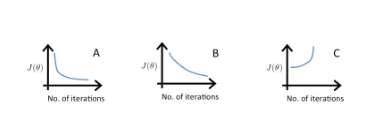
\includegraphics[width=0.9\columnwidth]{ml_figures/convergence.png}

A - good convergence

B - slow convergence

C - learning rate too high

Run GD with $\alpha$ with a range of values with 10-scale factor  3x from previous values

Until you find one value which is too small and one value which is too large

\subsubsection{Momentum}

\subsubsection{Netwon}

\begin{itemize}
\item no learning rate
\end{itemize}

For a function $l$ with the derivative $l^\prime(\theta)$ and second derivative, starting from an initial guess the update rule is:

$\theta := \theta - \frac{l^\prime(\theta)}{l^{\prime\prime}\theta}$

until $l^\prime(\theta)=0$. 

Newton method looks at the approximated tangent to $l(\theta)$ at the point $\theta$ and solves for where the line is equal to 0.

\subsubsection{Newton Raphson Method}

Generalization of Netwon's method to multi-variable / multi dimension settings:

$\theta = \theta - H^{-1}\nabla_\theta l(\theta)$

where $\nabla_\theta$ is a vector of partial derivatives of $l(\theta)$ with respect to $\theta$ and 

$H(\theta)=\frac{\partial^2 l(\theta)}{\partial \theta_i\partial\theta_j}$

Better and faster convergence than GD, but expensive, requires (careful) evaluation, Hessian needs to be invertible (full rank)

Fischer scoring - applying Newton's to logistic regression log likelihood function

\subsection{Polynomial Regression}

Basically, the idea here is to cheat and pre-compute the feature vector. 

For example, $(x_1 := x, x_2 := x^2, x_3 := x^3)$. 

The previous formulation and update rules hold: $\theta^Tx$

In this case it's important to scale the variables!

Other options: sqrt, cubic, squared (which might not fit a lot of models)

\subsection{Normal Equation}

For a feature vector $n$ features and $m$ data points: 

Construct a matrix $X  \in \mathbb{R}^{m\times (n+1)}$ which contains all of features for all the variables + (n+1) column which contains all 1s.

$\left( \begin{matrix} 1 & x_1^1 & ... & x_1^n \\ \vdots & x_2^1 & ... & x_2^n \\   1 & x_m^1 & ... & x_m^n \\ \end{matrix} \right)$

And collect all of the observations in a vector $y \in \mathbb{R}^m $:

And we solve for a model:

$\theta = (X^T X)^{-1} X^T y$



Now, this is true only if $X^T X$ is invertible

Feature scaling is not necc. when using the normal equation.

\subsection{GD vs. Normal Equation}

GD
\begin{itemize}
\item need to choose learning rate
\item need many iterations
\item works well when $n$ is large
\end{itemize}

Normal Equation 
\begin{itemize}
\item slow for large $n$  $O(n^3)$, n=10k is where switching over could be beneficial
\item no need to choose learning rate
\item direct
\end{itemize}

\subsection{When is $X^TX$ non-invertible?}

\begin{itemize}
\item linearly dependent features - i.e. size in $m^2$ and size in feet squared
\begin{itemize}
\item remove features
\end{itemize}
\item too many features $n\ge m$ 
\begin{itemize}
  \item delete features 
  \item use regularization
\end{itemize}
\end{itemize}

\section{Classification}

\subsection{Two Class Problems}
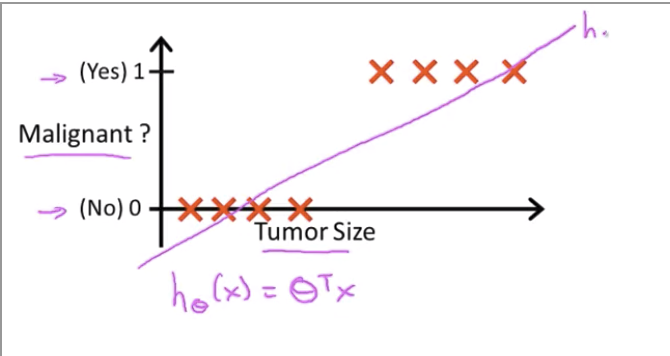
\includegraphics[width=0.9\columnwidth]{ml_figures/log_threshold.png}

Using linear regression model + threshold:

Classification is not actually a linear function - using linear models doesn't work well.

Labels are usually {0,1} known as negative and positive classes.

\subsubsection{Logistic Regression}

Want a model that predict a value $0\le h_\theta(x)\le 1$

Model: $h_\theta(x)=g(\theta^T x)$ 

Logistic/sigmoid function: $g(z) = \frac{1}{1+e^{-z}}$

Together: $h_\theta(x)=\frac{1}{1+e^{-\theta^T x}}$

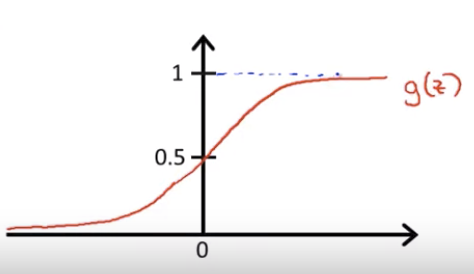
\includegraphics[width=0.9\columnwidth]{ml_figures/sigmoid.png}

Has  asymptotes at {0,1}

\subsubsection{Interpretation of Output}

$h_\theta(x)$ is the estimated probability that  $y=1$ on input $x$ 

$h_\theta(x) = P(y=1|x;\theta)$ 

$P(y=0|x;\theta) = 1-P(y=1|x;\theta)$

\subsubsection{Decision Boundary}

$g(z) \ge 0$.5 when $z>0$ 

$g(\theta^T x ) \ge 0.5$ when $\theta^Tx \ge 0$

(basically, here we  can derive this from $1+e^{-\theta^T x}  = 2$

The decision boundary is a function of the hypothesis and its parameters

\subsubsection{Non Linear Decision Boundaries}

Can perform a similar trick as with linear regression -> polynomial regression - build features such as $x_1^2$ etc...

So for example: 

$$\theta = \left[ \begin{matrix} -1 & 0 & 0  & 1 & 1 \end{matrix} \right]$$

$$h_\theta(x) = g(\theta^T(1,x_1,x_2,x_1^2,x_2^2 )) $$

The decision boundary will lie at $x_1^2 + x_2^2 = 1$

\subsubsection{Cost Function}

Using the linear regression cost function is non convex for the logistic regression.

$Cost(h_\theta(x),y) = \begin{cases} -\log(h_\theta(x))  ;\ \text{if} \;  y=1 \\ -\log(1-h_\theta(x))   ;\ \text{if} \;  y=0  \end{cases}$

This formulation has desirable properties: 

$(h(x)=0, y = 0)$ or$(h(x) = 1, y = 1)$  - cost = 0

Very high penalization if $(h(x)=1, y = 0)$ or$(h(x) = 0, y = 1)$ due to the cost function going asymptotically to $\infty$ :

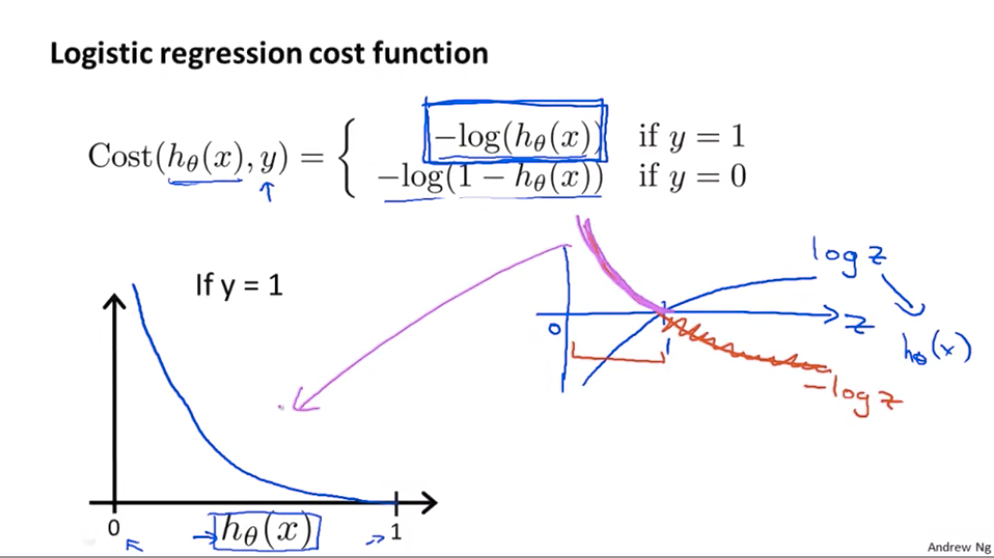
\includegraphics[width=0.8\columnwidth]{ml_figures/cost_function.png}

\subsubsection{Simplified Cost Function}

A generalized cost function is: 

$Cost(h_\theta (x), y) =-y\log(h_\theta(x))-(1-y)\log(1-h_\theta(x))  $

And summarizing over all examples:

$J(\theta)= -\frac{1}{m} \sum_{i=1}^{m} y^{(i)}\log(h_\theta(x^{(i)}))+(1-y^{(i)})\log(1-h_\theta(x^{(i)}))$

To minimize, solve for parameters:

$\min_{\theta} J(\theta) $ 

Output / new prediction: $h_\theta(x) = \frac{1}{1+e^{-\theta^T x}}$

$\frac{\partial}{\partial_{\theta_j}} J(\theta) = \frac 1 m \sum_i (h_\theta(x^{(i)})-y^{(i)})x_j^{(i)}$

Exactly the same update as linear regression. Here the main difference is that $h_\theta$  went from $\theta^T x $ to $\frac{1}{1+e^{-\theta^Tx}}$

And the update rules are:

$\theta_j := \theta_j - \frac{\alpha}{m} \sum_{i=1}^m (h_\theta(x^{(i)}) - y^{(i)}) x_j^{(i)}$

And vectorized:

$\theta:=\theta - \frac{\alpha}{m}X^T(g(X\theta)-\vec{y})$

\subsection{ Maximum Likelihood Estimation + Convexity}

Convexity: gives us lower bounds on the first order approximation of the function (i.e. the first order approximation is guaranteed to be larger than or equal to the real function value).

Assuming that the target variables and input are related via the equation: 

$y^{(i)}=\theta^Tx^{(i)}+\epsilon^{(i)}$

where $\epsilon$ are IID (independently and identically distributed) error terms the captures unmodeled effects, i.e random noise.

Assuming $e^{i}\sim\mathcal{N}(0,\sigma^2)=\frac{1}{\sqrt{2\pi}\sigma}\exp\left(-\frac{(\epsilon^{(i)})^2}{2\sigma^2}\right)$

That implies that: $p(y^{(i)}|x^{(i)};\theta)=\frac{1}{\sqrt{2\pi}\sigma}\exp\left(-\frac{(y^{i}- \theta^Tx^{(i)})^2}{2\sigma^2}\right)$ - this does not depend on $\theta$, the model is not a random variable! 

For the entire model's training set $X$  we can define this the **likelihood** function of the model : $L(\theta)=L(\theta;X;\vec{y})=p(\vec{y}|X;\theta)$

$L(\theta) = L(\theta;X,\vec y) = p(\vec y| X;\theta)$

Since all of the observations are independent:

$L(\theta)= \Pi_{i} p(y^{(i)}| x^{(i)};\theta) = \Pi_{i} \frac{1}{\sqrt{2\pi}\sigma}\exp\left(-\frac{(y^{i}- \theta^Tx^{(i)})^2}{2\sigma^2}\right) $

Maximum likelihood: we should choose a model $\theta$ so as maximize the probability of the data: $\theta$ should maximize $L(\theta)$. 

By deriving the function that maximizes $\log L(\theta)$ , product becomes a series sum and we simply need to maximize the $\frac 1 2 \sum_i (y^{(i)}-\theta^T x^{(i)})^2$ which is the original least-squares cost function.

Note that this does not depend on $\sigma$ !

\subsubsection{Maximum A Posteriori}

/TODO

\subsection{Locally Weighted Linear Models}

\subsection{Optimization Techniques}

There following algorithms are alternatives to GD that do not require choosing a learning rate:

\begin{itemize}
\item Conjugate Gradient
\item BFGS
\item L-BFGS
\end{itemize}

Advantages:
\begin{itemize}
\item No learning rate
\item Faster than GD
\item Line search
\end{itemize}

Disadvantages
\begin{itemize}
\item More complex
\item Prob. don't imp. yourself
\end{itemize}

\subsubsection{Multi-Class Classification Problems}

\subsubsection{One vs. All}

For example: tagging emails according to multiple classes; weather (rainy, sunny)

For each class, train a logistic regression classifier $h_{\theta}^{(i)}(x)$ that predicts that probability that $y=i$.

For new input choose $\max_ih_\theta^i(x)$

\section{ Overfitting vs. Bias}

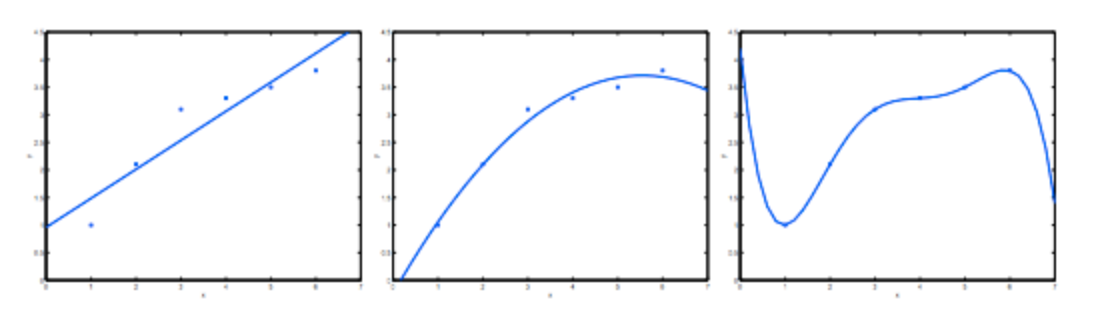
\includegraphics[width=0.5\columnwidth]{ml_figures/overfitting.png}
Underfitting -> high bias.

Overfitting, high variance

High variance - fitting a high order polynomial can be used to fit almost any function, not enough data to give a good hypothesis

If we have too many features, the learned hypothesis may fit the training data very well, but fail to generalize

\subsubsection{Addressing Overfitting}

Reduce number of features

Requires deciding which feature to keep and discard
Model selection algorithms

Regularization

\item keep features but reduce magnitude / values of $\theta_j$ 
\item works well when there are a lot features, each of which contributes less

Modify the cost function by penalizing the parameters:

Penalize higher order parameters: equiv to reducing the model to lower order model - simplfying the model

Penalize all parameters  - trying to keep the hypothesis small, usually corresponds to smoother functions

So now the objective has a data term and a regularization term.

The regularization term: $\lambda\sum_{j=1} \theta_j^2 $ keeps all of them small

If $\lambda $ is very large, in linear reg., all model params will be close to 0 and $h_\theta(x) = \theta_0$  


\section{Measuring Model Performance}

Type 1 Error - False positive - Predict an event when there was no event
Type 2 Error - False negative - Predict no event when in fact there was an event.

\subsubsection{Precision-Recall}

Precision-Recall curves summarize the trade-off between the true positive rate and the positive predictive value for a predictive model using different probability thresholds.

Precision-recall curves are appropriate for imbalanced datasets.

\subsubsection{ ROC -  Receiver Operating Characteristic curve

Summarize the trade-off between the true positive rate and false positive rate for a predictive model using different probability thresholds.

ROC curves are appropriate when the observations are balanced between each class

**Convolution** is a [mathematical operation](https://en.wikipedia.org/wiki/Operation_(mathematics)) on two [functions](https://en.wikipedia.org/wiki/Function_(mathematics)) (*f* and *g*) that produces a third function expressing how the shape of one is modified by the other

$(f\star g)(t) = \int_{-\infty}^{\infty} f(\tau)\cdot g(t-\tau)d\tau = \int_{-\infty}^{\infty} f(t-\tau)\cdot g(\tau)d\tau $

Commutative. 

For functions which only have limited support the integration is only done on the valid domain.

\subsection{L1 vs L2 Norm}

L2 norm strongly penalizes outliers. For good data with some very far outlier it might not generate the "best" fit as judged by a human observer.

L1 favors sparse coefficients.



\section{Support Vector Machines}

https://medium.com/machine-learning-101/chapter-2-svm-support-vector-machine-theory-f0812effc72\section{targetText=A Support Vector Machine (SVM,hyperplane which categorizes new examples.))



\section{Decision Trees}
Recursive repartition of the data

\subsection{Random Forest Regression}

An ensemble of decision trees. During learning tree nodes are split using random variable subset of data features.

All trees vote to produce final result.

For best results trees should be as independent as possible. Splitting using a random subset of features achieves this.

Averaging the product of the trees reduces overfitting to noise

5-100 Trees.

\subsection{Random Fern Regressors}



\section{Boosting}
Learning strong classifiers from weak classifiers.





\section{Naive Bayes Classifier}

/TODO

\section{RANSAC}

A method for dealing with noisy data. 

Partition the method 

Is not determinant, depends on the subset selection, and is not guaranteed to converge.

1. Select a random subset of the original data. Call this subset the *hypothetical inliers*.
2. A model is fitted to the set of hypothetical inliers.
3. All other data are then tested against the fitted model. Those points that fit the estimated model well, according to some model-specific [loss function](https://en.wikipedia.org/wiki/Loss_function), are considered as part of the *consensus set*.
4. The estimated model is reasonably good if sufficiently many points have been classified as part of the consensus set.
5. Afterwards, the model may be improved by reestimating it using all members of the consensus set.

```
Given:
    data – a set of observations
    model – a model to explain observed data points
    n – minimum number of data points required to estimate model parameters
    k – maximum number of iterations allowed in the algorithm
    t – threshold value to determine data points that are fit well by model 
    d – number of close data points required to assert that a model fits well to data

Return:
    bestFit – model parameters which best fit the data (or nul if no good model is found)

iterations = 0
bestFit = nul
bestErr = something really large
while iterations < k {
    maybeInliers = n randomly selected values from data
    maybeModel = model parameters fitted to maybeInliers
    alsoInliers = empty set
    for every point in data not in maybeInliers {
        if point fits maybeModel with an error smaller than t
             add point to alsoInliers
    }
    if the number of elements in alsoInliers is > d {
        % this implies that we may have found a good model
        % now test how good it is
        betterModel = model parameters fitted to all points in maybeInliers and alsoInliers
        thisErr = a measure of how well betterModel fits these points
        if thisErr < bestErr {
            bestFit = betterModel
            bestErr = thisErr
        }
    }
    increment iterations
}
return bestFit
```



\section{Bagging/Boosting}

Collaborative filtering

\section{Generative Models}

\section{Dimension Reduction}

\subsection{PCA}

\chapter{Unsupervised Learning}

Algorithms for finding structure in data.

\section{Clustering}

The clustering problem: given an unlabeled data set, group the data into coherent  subsets or into coherent clusters for us.

\subsection{K Means}

\item $K$ number of clusters + initialization
\item Training set ${x^{(1)},x^{(2)}\dots,x^{(m)}}$
\item $x\in\mathbb{R}^n$
\item By convention, drop $x_0=1$

```
Randomly initialize K cluster centers
While not converged:
1. iterate over data and assign a cluster for each data point based on distance to center
2. re-compute the cluster mean
```

If a cluster becomes empty - remove the cluster

Or randomly re-initialize the cluster

\subsubsection{K Means for Non Separated Clusters}

\subsubsection{K Means Cost Function}

Assuming: 

$c^{(i)}$ index of cluster to which the example $x^{(i)}$ belongs to.

$\mu_k \in \mathbb R ^n $ cluster centroid 

$\mu_{c^{(i)}} \in \mathbb R ^n $ location of the cluster centroid to which example $x^{(i)}$ has been assigned

Example cost for point $Cost(x^{(i)}) = \|x^{(i)} - \mu_{c^{(i)}} \|^2$ 

$J(c^{(1)},\dots, c^{(k)})= \frac{1}{m}\sum_i \|x^{(i)} - \mu_{c^{(i)}} \|^2 $

The objective is to minimize the cost function *distortion* with respect to the clusters (both labelling and centers).

So what k-means algorithm is actually doing is:

1. minimize the cost function with respect to cluster assignments $c^{(i)}$
2. minimize the cost function with respect to cluster centroids $\mu_k$ 

(so basically block coordinate descent?)

\subsubsection{Random Initialization}

\begin{itemize}
\item $K < m$
\item Randomly pick $K$ training examples and set the cluster means to these examples
\end{itemize}

K-mean can get stuck in a local optima - to avoid this a good option is to run k-mean multiple times and get as good global optimum

For multiple initializations - run K-means loads of times, pick the clustering which results in the lowest cost function

This works well for small $K < 10$ .

For large $K$s it is not as effective.

\subsubsection{Number of Clusters - Elbow Method}

Choosing the right K 

Plot the cost function with respect to the number of clusters.![elbow](/Users/kozlovy/Documents/2019_JobApplications/Notes/ml_figures/elbow.png)

In practice it is usually a bit harder, and it is not clear that there is such a transition where the distortion stops.

\section{Dimensionality Reduction}

\subsection{PCA}

PCA is trying to find a lower dimension representation of that data which minimizes the squared distance error of the data from the representation.

Before PCA it is standard practice to perform mean normalization and feature scaling. 

\subsubsection{PCA vs Linear Regression}

<img src="/Users/kozlovy/Documents/2019_JobApplications/Notes/ml_figures/PCA_Linear.png" alt="PCA_Linear" style="zoom:50%;" />

We do not treat $y$ as a special variable

Minimized projected error vs. minimize distance from line

\section{GMM and EM}


\section{Data Generation Using Simulation}

Generating good synthetic data: 
realism, 
diverse,


Want to render images which are as different as possible from each other

Parametric model of humans - procedural generation

\section{Neural Networks}

http://karpathy.github.io/neuralnets/


\section{ML Algorithm Design}

General process of building a ML product:

\begin{enumerate}
\item What is the objective? prediction, recommendation, clustering, search, etc.
\item Pick the right algorithm: supervised vs unsupervised, classification vs regression, generalized linear model / decision tree / neural network / etc.
\item Pick / engineer relevant features based on available data.
\item Pick metrics for model performance.
\item Optionally, comment on how to optimize the model for production.
\end{enumerate}

% %!TEX root = cv_ml_notes.tex
\section{Image Processing}

\subsection{Norms}

$L_1$ norm

$L_2$ norm

Huber’s norm

$L_\infty $

\section{Computational Photography}

Bayer Pattern


\section{Image Analysis}

\textbf{Hough transform} - line representation - line equation and radial.

\subsection{Integral Images}

The value at any point $(x, y)$ in the summed-area table is the sum of all the pixels above and to the left of (*x*, *y*), inclusive where $i(x,y)$  is the value of the pixel at $(x,y)$. The summed-area table can be computed efficiently in a single pass over the image:

$I(x,y) = i(x-1,y-1) + I(x,y-1) + I(x-1,y)-I(x-1,y-1)$

and similarly for any rectangular region:

$ i(A,B,c,D) = I(D) - I(B) - I(C)+I(A)$

\section{ Filtering}

Peak Signal To Noise Ratio 

\begin{itemize}
\item Color Conversion
\item Thresholding
\item Smoothing
\item Morphology
\item Gradient
\end{itemize}

\subsection{Sobel Operator}

Uses $3\times3$ operators which are convolved with the image to compute approximate (center difference?) derivatives in $x$ and $y$ directions.

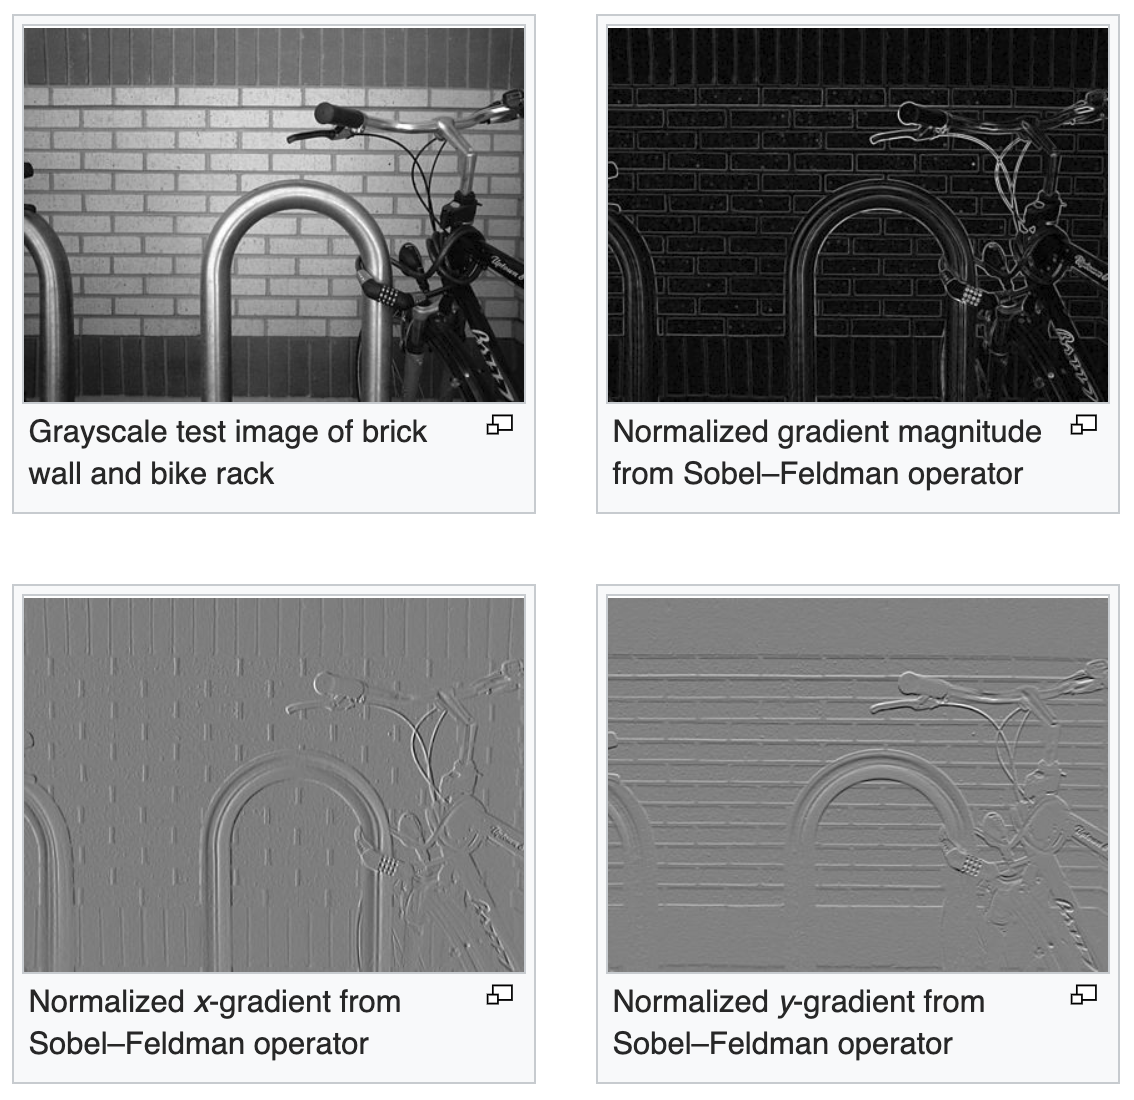
\includegraphics[width=0.9\columnwidth]{img_proc/sobel.png}

\subsection{Canny Edge Detection}
\begin{enumerate}
\item Apply Gaussian filter to smooth the image in order to remove the noise
\item Find the intensity gradients of the image
	The edge orientation is the atan of the intensity of the gradient in each dimension
	The edge magnitude is the sqrt
\item Apply non-maximum suppression to get rid of spurious response to edge detection
\item Apply double threshold to determine potential edges
\item Track edge by hysteresis: Finalize the detection of edges by suppressing all the other edges that are weak and not connected to strong edges.
\end{enumerate}

\textbf{Contours}
\textbf{Histograms}

\subsection{Convolution}

\section{Image Deblurring}

\section{Fourier Transform}

\section{Image Compression}

\section{Optic Flow}

\subsection{Gaussian Pyramids}

Gradient consistency assumption + intensity consistency assumption

Iterative multi scale + warping

Uses an analytic formulation derived from Euler-Lagrange Equations

Results in a dense optic flow field.

Works well for small changes.

\section{Interpolation}

\subsection{Nearest Neighbor}

\subsection{Bilinear Interpolation}

Linear interpolation on a 2D grid. 

\section{Noise Models}

\subsubsection{Salt and Pepper / Black White}
This type of noise happens due to sudden interruption in the image signal.
Also known as data drop noise because statistically its drop the original data values
Can be removed using median or morphological filtering.

\subsubsection{Gaussian noise}
Noise which has a probability density function (PDF) equal to that of the normal distribution.
Can be estimated by taking a dark image and measuring the variance of the pixels. Removed by smoothing.

\section{Semantic Computer Vision} 

Visual Odometry

\section{Silhouette Segmentation / Visual Hull}

\section{Optic Flow}

\section{Image Segmentation / Pixel Labeling}

\section{Object Detection}

\section{Classification Problems}

\section{Event Cameras}

\subsubsection{Features}

\begin{itemize}
\item Low-latency ($\sim1 \mu s$)
\item No motion blur
\item High dynamic range (140 dB instead of 60 dB)
\item Ultra-low power (mean: 1mW vs 1W)
\end{itemize}

Traditional vision algorithms cannot be used because:
\begin{itemize}
\item Asynchronous pixels
\item No intensity information (only binary intensity changes)
\end{itemize}

But they bring new possibilities:
\begin{itemize}
\item Night vision
\item Compact representation and data
\end{itemize}

On static scenes, they mostly produce noise

Main visible features - edges. 

\subsubsection{Linearized Event Generation}

An event is triggered $\log I(x,t) \log I(xt-\Delta t)=\pm C$

Where $C$ is the minimal contrast which is required for triggering an event, scene dependent.

Consider a pixel $p(x,y)$ with gradient $\nabla L(x,y)$ undergoing a motion $u\in(u,v)$ induced by a moving point $p \in\mathbb{R}^3 $

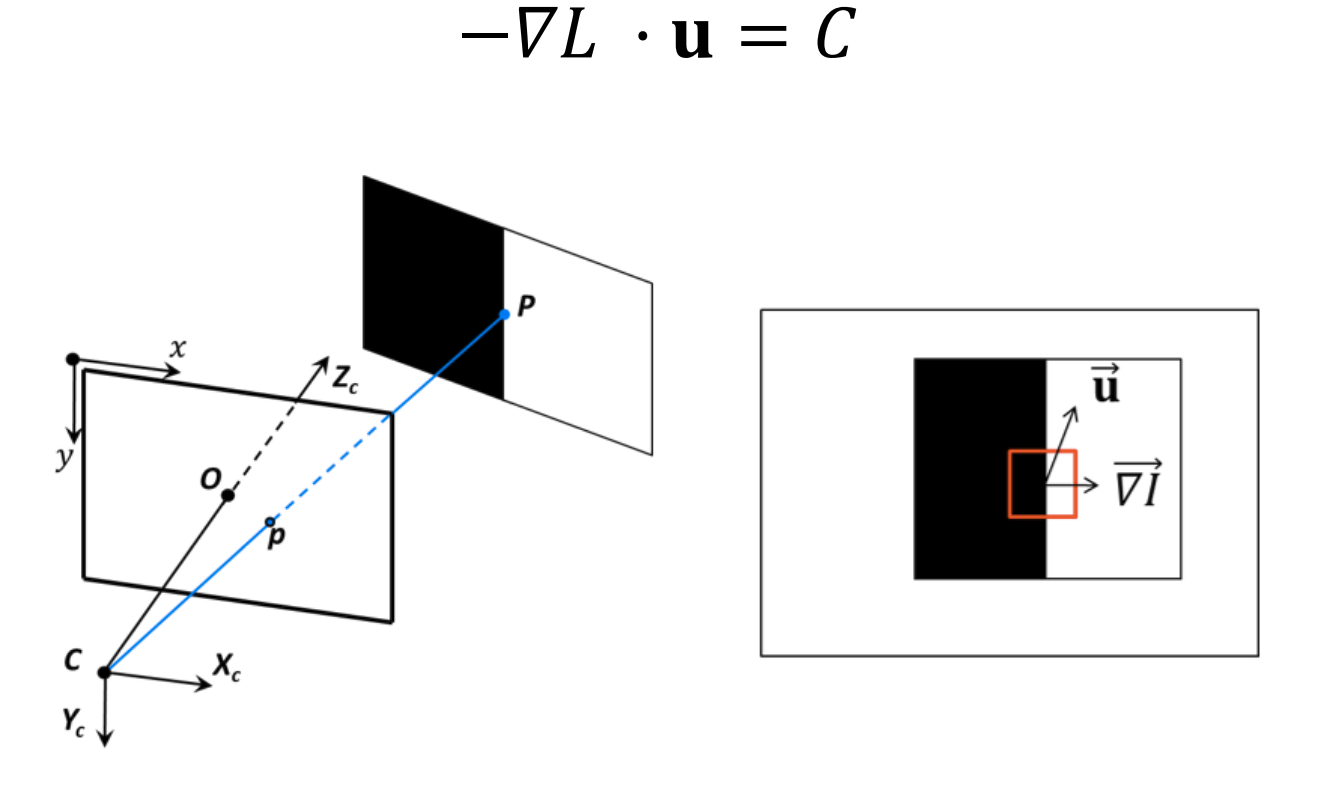
\includegraphics[width=0.9\columnwidth]{event_cameras_fig/event_cameras.png}

From brightness constancy assumption:

$L(x,y,t) = L(x+u,y+v,t+\Delta t)$ from first order approx we get the following $-\nabla L \cdot \vec u = C$

\subsubsection{Deblurring}

A blurry image can be regarded as the integral of a sequence of latent images during the exposure time, while the events indicate the changes between the latent images.

Sharp images are done by subtracting the double integral of the events

\subsubsection{(Sparse) Feature Tracking In Event Space}

\subsubsection{Kanade–Lucas–Tomasi}

Goal: extract features on frames and track them using only events in the blind time between two frames

Uses the event generation model via joint estimation of patch warping and optic flow

Disadvantages: requires GPU for real time tracking and they require knowledge of contract sensitivity, which is scene dependent and differs from pixel to pixel.	

\subsubsection{Image Reconstruction from Event Cameras}

Recurrent neural network (main module: Unet) 

Input: last reconstructed frame + sequences of event tensors (spatio-temporal 3D voxels grid: each voxel contains sum of ON and OFF events falling within the voxel)

Network processes last $N$ events (10,000) 

Trained in simulation only (without seeing a single real image) (we used our event camera simulator: \url{http://rpg.ifi.uzh.ch/esim.html} Noise free simulation with randomized contrast sensitivity.

% \refstepcounter{chapter}
\chapter{Geometry Processing} 

\section{Basics}

Plane normal equation

Plane point distances

Barycentric coordinates


\section{ Surface Representations}

Explicit:
\begin{itemize}
\item Mesh
\item Spline surface
\item Oriented planes
\item Point cloud
\end{itemize}

Implicit - voxel grid:
\begin{itemize}
\item Signed distance fields (implicit) <0, 0, >0
\item Signed distance fields (implicit)
\item Occupancy grid
\item Signed-distance grid
\item Voxel octree
\item Tetrahedral Mesh
\end{itemize}

Volumetric modeling for vision:
• Flexible and robust surface representation
• Handles (changes of) complex surface topologies effortlessly
• Ensures watertight surface / manifold / no self- intersections
• Allows to sample the entire volume of interest by storing information about space opacity
• Voxel processing is often easily parallelizable


Drawbacks:
Implicit surface representation

\subsection{Marching Cubes}
Recovers an isosurface from a volume
ensures a watertight surface
Can be done per voxel
15 combinations of surface intersections per cube
Precise normal specification
Accuracy depends on resolution

Trivial merging or overlapping of different surfaces based on the corresponding implicit functions:
• minimum of the values for merging • averaging for overlapping

Limitations of Marching Cubes
• Maintains 3D entries rather than a 2D surface, i.e.,
higher computational and memory requirements
• Generates consistent topology, but not always the topology you wanted
• Problems with very thin surfaces if resolution not high enough


\section{ICP}

Algorithm:

\section{Point Cloud Merge}

ICP for point cloud matching

Normal Estimation

Outlier detection / removal 

Surface / mesh fitting / template fitting

\subsubsection{Geometric Representations}

Bezier curves

\section{Laplacian Deformation}
%!TEX root = computer_vision_notes.tex
\section{Deep Learning for Computer Vision - Lecture Notes}

ImageNet
CIFAR10

Training - expensive
Test - should be cheap 

Regression functions predict a quantity, and classification functions predict a label.

So for example, NN labeling based on pixel diff is bad, because training is cheap and evaluation is expensive
Also suffers from: tint, shift, do not correspond well to perceptual similarities

$L_1$ distance depends on coordinate system 

For testing hyperparamters (for example, K-nearest neighbors, etc):
- train, validate and test data tests. Hyperparamters are optimized on the validation dataset

Cross validation - 
used for small datasets, less for deep learning
data is split into folds
hyperparameters are averaged over the different fold choices
higher confidence on which hyperparameters are used

Data sets should probably be created with the same probabilistic distribution

The curse of dimensionality:
\# of training examples is exponential to the \# of pixels for examples, if we use pixel dist as the descriptor

kNN is a parametric model

\subsection{Linear Classification}

image(x) -> f(x,W) -> 10 numbers of scores per class
W are parameters, so this is what we're learning

deep learning - how to get this function f

linear classifier - f = Wx + b 
b is the bias term, which can give class preferences for one class over another, can be used to unbias an unbalanced dataset

We can visualize the linear classifier to have some idea for template matching

Linear classifier only learn one appearance for each class. It does not deal with variation in class appearance

linear classifier try to create a linear barrier in a high dimension space between classes	

Examples where linear classifiers fail:
multi model data
one class that can appear in different areas of space
for example: 1 < l2 < 2


\subsection{Loss Functions}

The loss function measures how much error we have in our classification

\subsubsection{Multi Class SVM - Generalization of Binary SVM }

Loss is 0 if the incorrect label is lower than correct label + safety margin
or wrong-score - correct-score + safety-margin = $\max(0, s_{wrong} - s_{correct} + safety)$
This is summed only over the wrong categories

Also known as hinge loss

After initialization W is small, initialize by setting all params to more or less similar: 
so the first loss should be approx. $C-1$ where $C$ is the number of categories

squared hinged loss will create a different classifier because the trade off between good and bad scores is different

hinge loss - we don't care if it's a little bit wrong or very wrong, but squared hinge loss heavily penalizes outliers

The loss function is how we design which errors the algorithm cares about

If we have loss = 0, the classifier is not unique, should be scalable 

Also the loss should not depend only on fitting the training data.

This is solved by regularization, which encourages the model to use a "simple" W
What is simple? that depends on the regularization term which you choose

\subsection{Multinomial Linear Regression}

Now the scores actually have meanings, they're the unnormalized log probabilities of the classes

softmax function - exp of the score ensures positivity
$ P(Y=k|X=x_i) = \frac{e^{s_k}}{\sum_j e^{s_j}} $

Want to maximize log likelihood, minimize the negative log likelihood of the correct class
So the loss function is:
$ L_i = - log P(Y=y_i|X=x_i) $
minus log of the probability of the true class
$ L_i = - log \frac{e^{s_{y_i}}}{\sum_j e^{s_j}} $

\subsection{Multinomial Logistic Regression}

To get perfect loss function, we need infinite scores for the correct class and minus infinity scores for the wrong class

min loss is 0 
max loss is infinity

when all classifiers are ~0, the first iteration should be log(c)

cross entropy loss
- log probability of the correct class

softmax wants to push the probability towards 1.0 (or score toward infinity) and other class towards negative inifinity. so even small changes of the scores of the classes will change the loss function

score function vs. loss function

Computing finite differences is terrible idea, because very slow due to high dimensions of the function

Numeric gradients are error prone.
Always validate with finite differences. 

\paragraph{Gradient Descent}

Step size or learning rate is one of the most important hyper parameters

Stochastic gradient descent

Momentum method

ADAM optimizer

Computing the loss might be very expensive if we use all of the examples in our training / validation sets

The analytic gradient of the loss is very slow to compute

Stochastic Gradient Descent - at every step compute a minibatch which is a $2^n$ examples
Estimate of the true gradient

\subsection{Back Propagation}
Once we  can express something as a computation graph we can use a technique called back-propagation

The loss is at the bottom

\subsubsection{Gates}
Add gate - gradient distributor 
Max gate - gradient router
Mul gate - gradient switcher

When one node is connected to multiple nodes, the gradients are added at this node.

$\frac{\partial f}{\partial x} = \sum_i \frac{\partial f}{\partial q_i}\frac{\partial q_i}{\partial x} $

So now we do this for vectors, Jacobians and Hessians:

The size of the Jacobian is the dimension of the input vector times the dimension of the output vector. for minibatches the jacobian is even larger - 400kx400k easy... 

If the gates are element wise, the Jocobian is a diagonal matrix

Exercise: What's the gradient of the L2 norm? 

\subsubsection{Sigmoid function:}
$\sigma (x) = \frac{1}{1-e^{-x}}$

Exercise: break down the sigmoid function into gates
Compute the back propagation

The gradient with respect to a variable should have the same shape as the variable

How to Build Neural Networks

Fully connected linear layers - all outputs of one layer are connected to all inputs of a second layer
The abstraction of layer allows for matrix - vector operations


 \subsection{Neural Nets - History Recap}

 Krizhevsky 2012 - first use of modern neural networks on Imagenet that generated good results


 1980s - Experiments on Vision in Cats: 
 - nearby regions in vis cortex represent nearby region in vis field
 - neurons had heirarchical org 

Simple cells - response to light and orientation 
Complex cells - light, orientation and movement 
Hypercomplex - movement with an end point

Complex cells sort of do pooling

1998 - gradient based learning applied to document recognition

2012 - modernized version
dense connections 
max connections between layers

\subsection{Layer Types}

\subsubsection{Fully Connected Layers}

Image 32x32x3 -> stretch out all pixels to a single vector x = 1x3072 
Layer W 10x3027
Wx = activation per "neuron" -> 1x10

Fully connected layers are used to compute max scores

\subsubsection{Convolution Layers}
Preserve spatial structure: 
32x32x3 x 
and the filter is going to be 5x5x3 
compute dot product at every spatial location

Filters always extend the full depth of input volume

The dot product is called activation - which is the size of the image - filter + 1

The structure usually follows something like this:
CNN
Pool
CNN
...

\paragraph{Strides}

Used to reduce dimensionality

Stride size - the interval of sampling locations

Stride and image size need to match: (N - F) / Stride + 1 

\# of parameters per filter - $size_x \times size_y \times depth - 3$

It is common to pad the borders to get the appropriate size

This is also known as receptive field

\subsubsection{Pooling layers}

Reduces representation size, s.t. it is more manageable 
Pooling is only in the spatial, not over depth
Max pooling is commonly used (also softmax)

The pooling layer is controlled by three hyperparamters:
Spatial extent 
Stride 

Produced $w_2 \times h_2 \times d_1$
$w2 = (w1 - f)/s + 1$
$h2 = (h1 - f)/s + 1$
$d2 = d1$

introduced zero parameters
zero padding isn't usually used

Common parameters:
$f=2, s=2 $

$f=3, s=2$

\section{Training Neural Networks}

\subsection{Activation Functions}

\paragraph{Sigmoid function $\frac{1}{1+e^-x}$}
Maps all variables to [0,1]
Interpetation - saturating firing rate of a neuron 

Disadvantages:
- saturated neutron kill off the gradients - when doing backpropagation for large values, i.e. let's say $x = \pm10 $ the gradient is simply going to be 0 
- the maximal gradient is obtained at $x = 0.5$ 
- sigmoid outputs are not 0-centered - this means that the gradient computed is always either all positive or all negative. as a result, the this means that the optimization cannot always step in the true direction of the gradient, but wil take a zig zag path. so it's important to have 0-mean input
- exponential function - expensive.

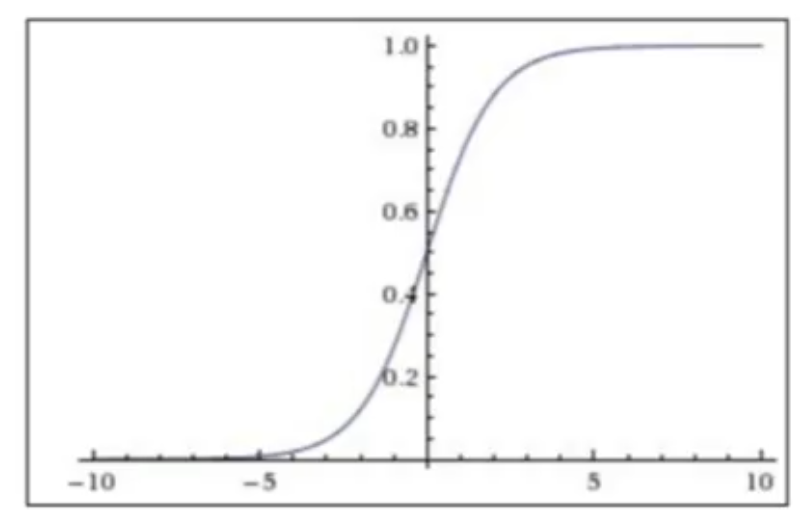
\includegraphics[width=0.5\columnwidth]{fei_fei_li/lecture_06/sigmoid.png}
tanh - $tanh(x)$ 

- Similar to sigmoid function
- the output is in the range of [-1,1]
- zero centered
- gradient = 0 when saturated

\paragraph{ReLU - $f(x) = max(0,x)$ }

- Rectified Linear Unit
- Does not saturate in the positive region
- Very computationally efficient
- Converges much faster than sigmoid and tanh (x6)
- More biologically plausible than sigmoid

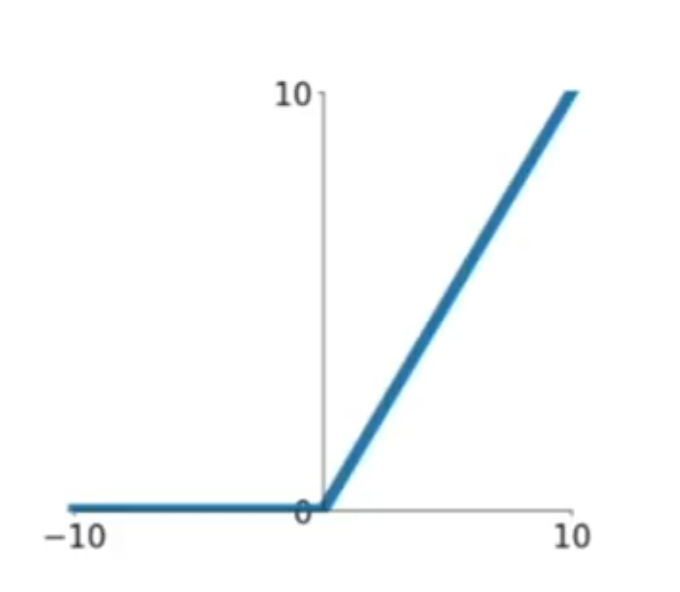
\includegraphics[width=0.5\columnwidth]{"fei_fei_li/lecture_06/Screenshot 2019-10-18 at 13.31.23.png"}

 Disadvantages

- does kill the gradient in the negative part of the regime
- It is possible to have dead ReLU that do not activate or update for a large part of the data. This can happen due to the following reasons:
  - bad initialization
  - learning rate is too high - large updates and the weights just around fast, the ReLU can get knocked off the data manifold

\paragraph{Leaky ReLU - $f(x) = max(0.01x, x)$ }

- Instead of being flat in the negative regime, it returns a negative gradient
- This solves the saturation problem and improves the convergence rate
- Computationally efficient

\paragraph{PReLU $f(x) = max(\alpha x, x)$}

- The $\alpha$ becomes another parameter
- Improves flexibility

\paragraph{Exponential Linear Unit (ELU)}

$$ f(x) = \begin{cases} x & \text{if} x > 0 \\ \alpha(exp(x)-1) & \text{if} x < 0 \end{cases}  $$ 

- expensive - requires an exponent
- this build back saturation in the negative regime 
- possible interpetation is that this is more robust to noise
- this is between relus and leaky ReLUs

\paragraph{Maxout $\max(w_1^Tx + b_1, w_2^T x + b_2)$}

- Generalization of ReLU and Leaky ReLU
- Linear regime 
- No saturation
- Doubles the number of parameters per neuron

\subsubsection{Guidelines to using activation functions }

- ReLU is the standard
- LReLU / Maxout / ELU are ok to try
- tanh can be used very carefully
- Don't use sigmoid :( original activation function - but people advanced to ReLU

\subsubsection{Data Processing Pipeline}

1. original data
2. zero - meaned data
3. normalized data - according to the std in each dimension
   - we need 0-mean data because any sort of bias will cause bias and (maybe) reduce the convergence

Approaches to normalize the data can include:

	- PCA - the data has diagonal covarriance matrix 
	- whitened data - the covariance matrix is identity
	- with images - stick to normalization, projecting pixel values into a lower dimensionality representation might not be beneficial
	- want to preserve spatial structure
	- training and test data are normalized in the same way
	- options include - subtract the mean image
	- subtract the per-channel mean

\subsubsection{Approaches to Initializing the NN:}

 - Setting initial nets - if all of the weights are 0 all of the neurons will respond in the same way, will all get the same gradient. 

 - Set initial weights to a small value that we sample from a normalized (Gaussian) with 0 mean W = 0.01*np.random.randn()
   	
   	- This works for small networks but does not work for deeper network
      	
      	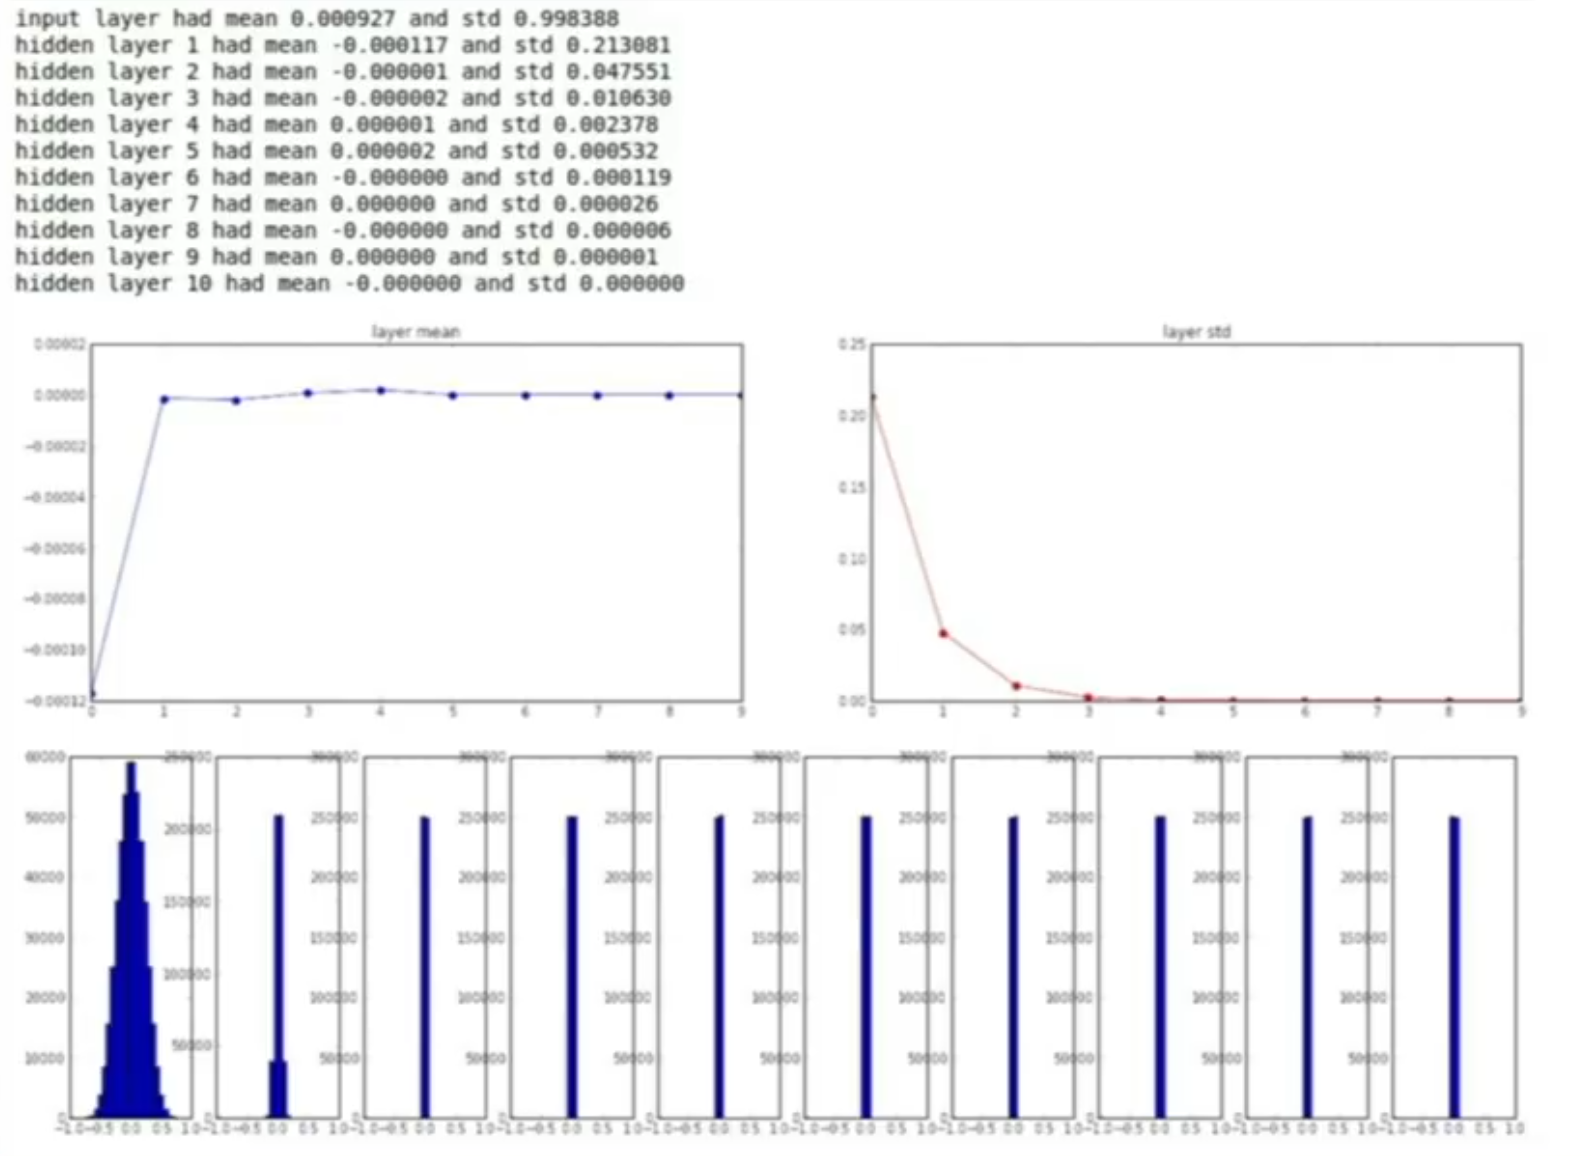
\includegraphics[width=0.5\columnwidth]{fei_fei_li/lecture_06/ecture_06_normalized-activation.png}
    
   - The mean for all of the layers is going to be zero which makes sense 

   - The STDEV shrinks at each layer and quicly collapses to 0 

 - Setting initial weights to large values - 
   	
   	
   
   - All of the neurons are going to be in the saturated regime, leading to values of $\pm1$ 
   
 - Xavier initialization - from Glorot
    - ${fan_{in}}$ - number of inputs
    - sample from a gaussian
    - normalize by the number of inputs
    - $W = random(min,max)/sqrt(min)$
    - variance of the input is equal to the variance of the outputs
       - small number of inputs - larger weights
       - large number of input - smaller weights
    
 - This reasonable initilization - math derivation assumes linear activation

 - But this breaks when you use a ReLU
   	
   	- the ReLU kills half of the neurons - sets the weights to 0 
    
   - changes the variance - so you can divide by 2 and this improves the weights

    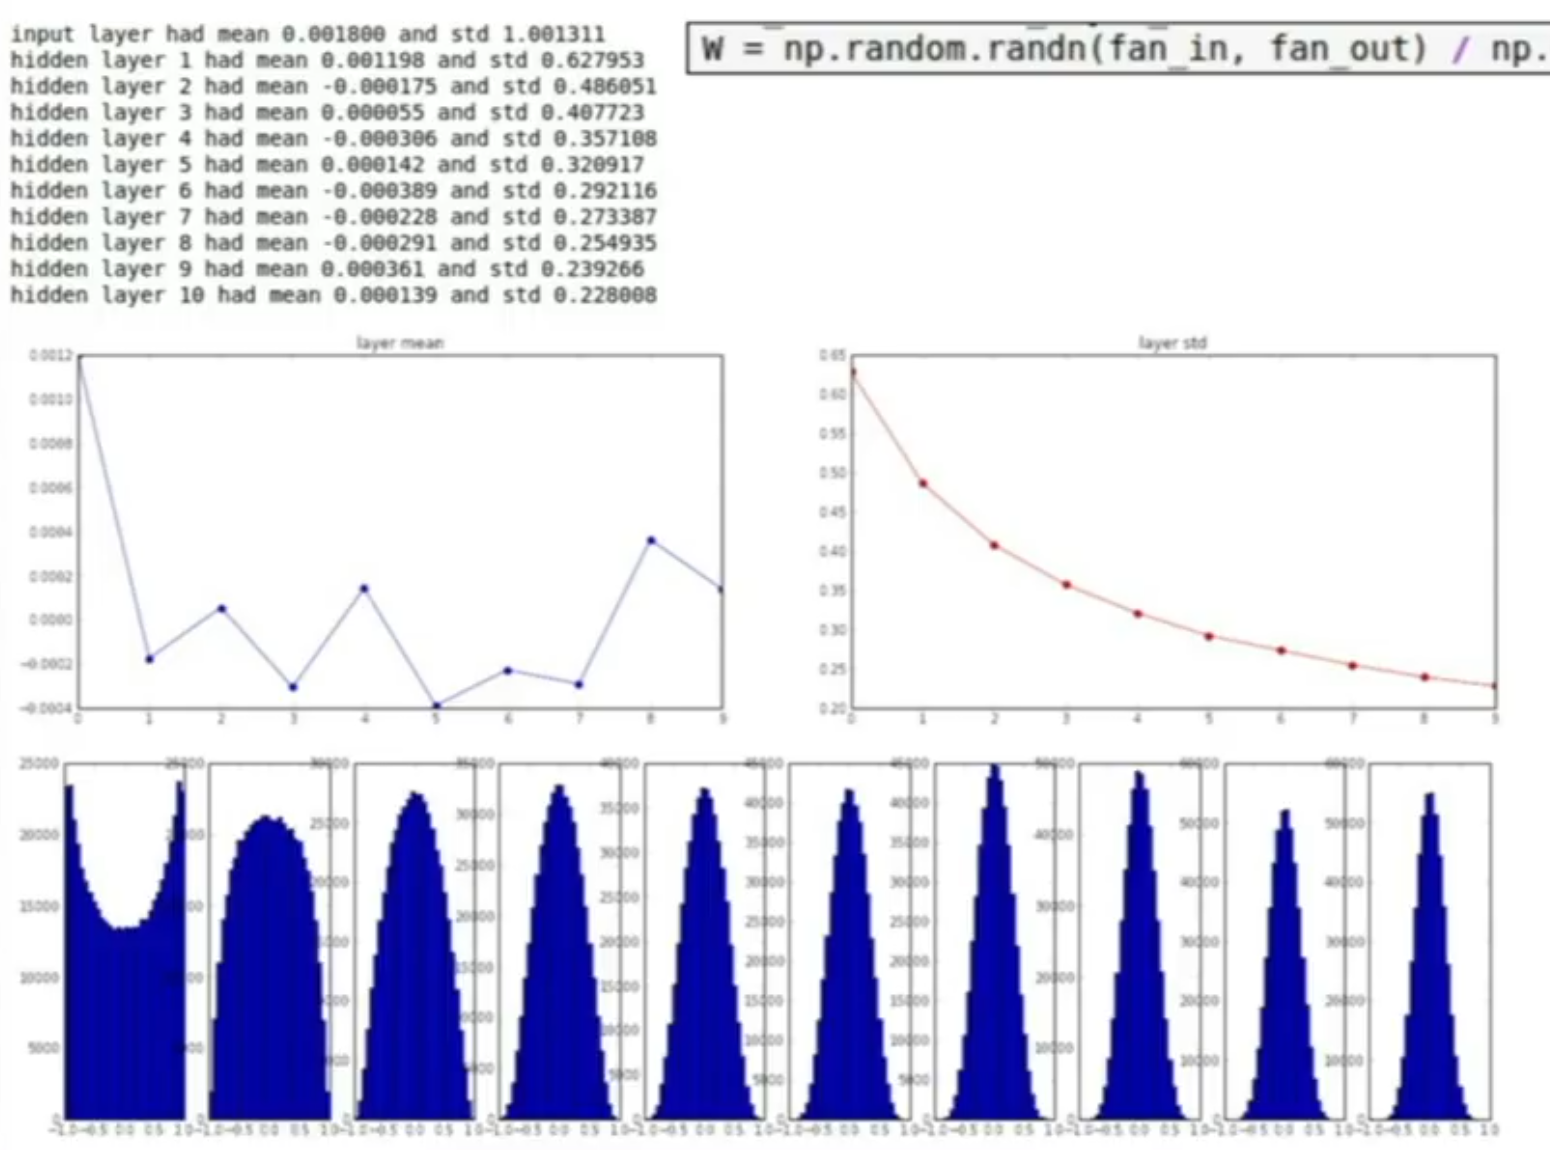
\includegraphics[width=0.5\columnwidth]{fei_fei_li/lecture_06/xavier_init_vis.png}

\subsubsection{Batch Normalization}

Consider a batch of activations at  some layer - make each dimension unit gaussian:

$$\hat x^k = \frac{x^{(k)} - E[x^{(k)}] }{\sqrt{\text{Var}[x^(k)]}} $$

which is differentiable

This is done per-dimension

The step is usually done after each fully connected layer and convolutional layers - to mitigate bad scaling effects at each layer

For convolutional layers - we also want to normalize jointly all spatial dimensions and all of the training examples - i.e. we want nearby locations to be normalized in the same way - one mean and one stdev for one actibation map we have. 

Check out **Ioffe and Szegedy, 2015** and understand the paper and the methods they present. 

We might not necc. want unit Gaussian input to the tanh layers: this constraints you the linear regime of the non-linearity.



We can add a scaling and shifting operation - but the network can learn a scaling $\gamma = \sqrt{Var(x)}, \beta = E[x^k]$ which is the identity mapping

$y^{(k)} = \gamma^{(k)}\hat{x}^k + \beta^{(k)} $

Improves gradient flow through the network 

More robust - higher learning rates and diff. init.

Regularization - each of the outputs is dependent on the inputs as well as the outputs of all images in the batch



At test time the batch norm functions differently: a single fixed mean of activation during training is used (can be estimated during training with running averages)

\subsubsection{Monitoring Training }

1. Preprocess the data

2. Choose the architecture

   1. input - hidden layer - output

3. Validation - step 1 - ensure loss is reasonable 

   1. disable regularization
   2. do a forward pass
   3. test the loss is reasonable
   4. for example for softmax the "correct" loss is about -log likelihood

4. Regularization validation

   1. add reg. 
   2. observe the loss increases

5. Validate arch works:

   1. start with a very small set of data
      - small set - be able to fit the data very well.
      - turn off reg
      - use simple vanilla sigmoid
   2. ensure that the loss can go down to 0 and training accuracy goes up to 1

6. Figure out the training rate (step size):

   - start with small regularization and find the learning rate to make the loss go down
   - in early stages of learning with softmax, even though the loss does not change much, we can observe large jumps in accuracy because small shifts in labels can lead to large changes to the classification with softmax
   - NaN - learning rate too high
   - A good range [1e-3, 1e-5]

7. Hyperparameter Optimization

   Cross validation in stages, coarse to fine

   Best to optimize in log space

   - Stage 1:
     - try a few epoch instances
     - pick values spread out apart
   - Stage 2:
     - longer running time, finer search
   - Solver explosion detection: 
     - if the cost is x3 original cost, quit
   - If all learning rates are at the edge of our hyperparameter sampling space, it means we might not have explored the range appropriately
   - Random Search vs. Grid Search (Begstra and Bengio, 2012)
     - Grid layouts 
     - Better to sample randomly from each parameters in the range
     - If a function is dependent more on one variable than another, which is usually true, because we have lower effective dimensionality than what we usually have, we will have more samples of the important factor - more useful signal
   - Hyperparameters:
     - network arch.
     - learning rate, decay schedule, update type
     - regularization (l2/dropout)

8. Bad Init - flat learning curve

9. Track ratio of weight update / weight magnitude - ratio of 0.01-0.001 is about good

\paragraph{Training a Neural Network}

1. Randomly initialize the weights
2. Implement forward propagation to get $h_\theta(x(i))$  for any $x^{(i)}$
3. Implement the cost function
4. Implement backpropagation to compute partial derivatives
5. Use gradient checking to confirm that your backpropagation works. Then disable gradient checking.
6. Use gradient descent or a built-in optimization function to minimize the cost function with the weights in theta.

\subsubsection{Stochastic Gradient Descent}

Normal gradient descent:

\begin{verbatim}
while True:
  weights-grad = evaluate_gradient(loss-fun, data, weights)
  weights += - step-size * weights-grad
\end{verbatim}


High condition number - cases of functions where the loss changes quickly in one direction and slowly in another direction. The ratio of the smallest to the largest singular value in the Hessian matrix

For functions such as this, there's a tendency to zig zag (valley problem), leading to slow convergence. This problem is more common in higher dimensions.

Local minima and saddle points:

SGD will get stuck because the gradient is 0.

Saddle points are common in high dimensions. The problem is also close to the saddle point.

Stochastic - the gradient and loss are estimated using a small number of example batches

Any noise in the gradient means that the optimization wanders around in the space and might take a lot of time to converge

Momentum term:

We step in the direction of our velocity and add friction

This simple strategy helps a lot.

Nesterov Estimated Gradient: 

Evaluate the gradient at the point where the velocity vector takes you, and mix the two to step again from the original point

tendency to overshoot minimum, nesterov tends to overshoot less.

flat minima are prob. generalizing better - recent theoretical work

feature, not a bug that sgd momentum skips over sharp minima

\paragraph{AdaGrad}

\begin{verbatim}
grad_squared = 0
while True:
  dx = compute-gradient(x)
  grad_squared += dx * dx 
  x -= learning_rate * dx / np.sqrt(grad_squared) + 1e-7)
\end{verbatim}

What it does: 

1. normalizes the relative step size in each dimension based on the history, so it will increase step size for variable with small gradient and dec step size for variables with high gradient
2. Over time the step size decays - in the convex case it is good. non convex case, it is problematic - you might get stuck with adagrad

\paragraph{RMSProp}
\begin{verbatim}
grad_squared = 0

while True:
  dx = compute_gradient(x)
  grad_squared += decay_rate*grad_squared + (1 - decay rate) * dx * dx
  x -= learning_rate * dx / np.sqrt(grad_squared) + 1e-7)
\end{verbatim}

0.9 or 0.99 decay rate.

estimates are leaky - not always slowing down?

RMS prob does not tend to overshoot as much, the optimization makes equal progress along all dimensions

AdaGrad decays quickly if the learning rate is fixed relative to other methods.

\paragraph{Adam}

Maintain an estimate of the first and second moment

Momentum

Bias correction

AdaGrad/RMSProp

If the valley problem is not xis aligned, non of the algorithms can deal with that (think squished taco)



let's compare Adam and AdaGrad/RMSProp with momentum:

\begin{verbatim}
first_moment = 0
second_moment = 0

while True:
  dx = compute_gradient(x)
  first_moment = beta1 * first_moment(1-beta1)              //momentum
  second_moment = beta2 * second_moment(1-beta1)*dx         //AdaGrad/RMSProp
  x -= learning_rate * first_moment / (np.sqrt(second_moment) + 1e-7 )  
\end{verbatim}

% \begin{verbatim}
% first_moment = 0
% second_moment = 0

% while True:
% ​	dx = compute_gradient(x)
% ​	first_moment = beta1 * first_moment(1-beta1)   						//momentum
% ​	second_moment = beta2 * second_moment(1-beta1)*dx					//AdaGrad/RMSProp
% ​	x -= learning_rate * first_moment / (np.sqrt(second_moment) + 1e-7 )	
% \end{verbatim}

And in fact full form Adam is: 

\begin{verbatim}
first_moment = 0 
second_moment = 0

for t in range(num_iterations):
  dx = compute_gradient(x)
  first_moment = beta1 * first_moment(1-beta1)   						//momentum

  second_moment = beta2 * second_moment(1-beta1)*dx					//AdaGrad/RMSProp
  first_unbias = first_momentum / ( 1 - beta1 ** t)
  second_unbias = second_momentum / ( 1 - beta2 ** t)
  x -= learning_rate * first_unbias / (np.sqrt(second_unbias) + 1e-7 )
\end{verbatim}


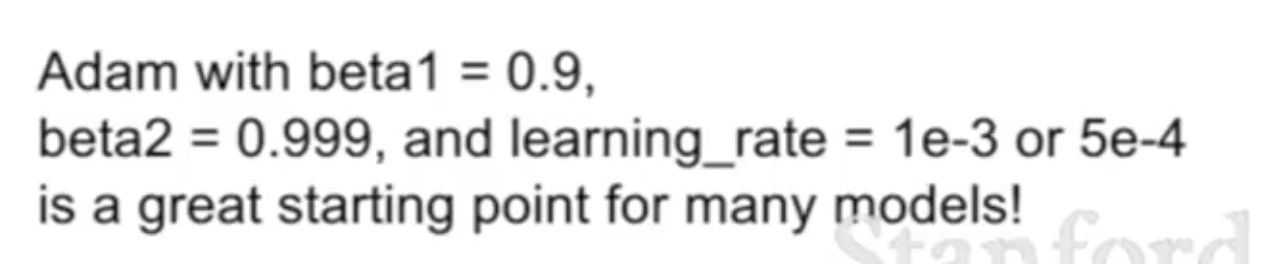
\includegraphics[width=0.5\columnwidth]{fei_fei_li/lecture_07/adam_params.png}

\paragraph{Learning Rate Decay}

Step decay - half the learning rate every few epochs

exponential decay - $\alpha = \alpha_0e^{-kt}$ 

1/t decay - $\alpha = \alpha / (1+kt) $ 

More Common with SGD and Momentum and less common with Adam

Start without learning rate decay

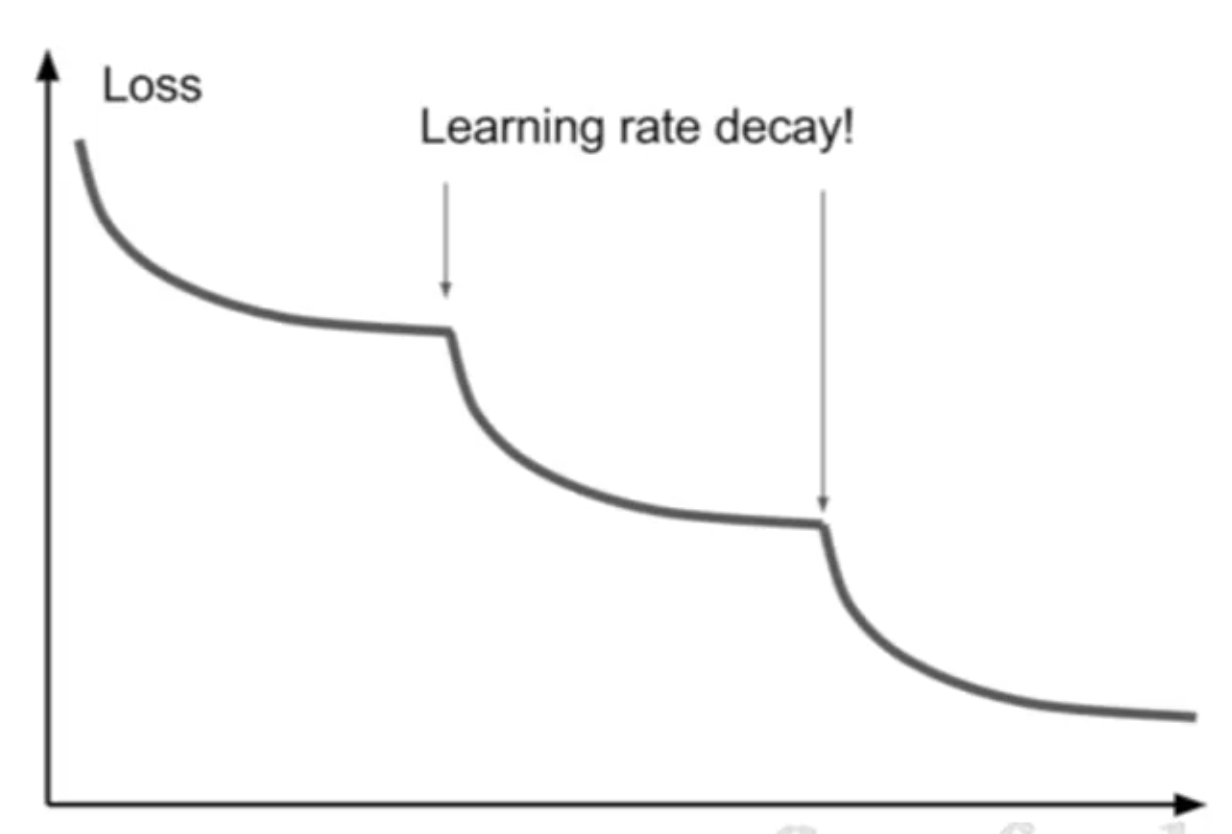
\includegraphics[width=0.5\columnwidth]{fei_fei_li/lecture_07/learning_rate_decay.png}

All of these algorithms are **First Order Optimization Algorithms**

1. Use gradient to approximate the derivative (in a linear manner)
2. Step to minimize approximation

The step does not hold for large step size

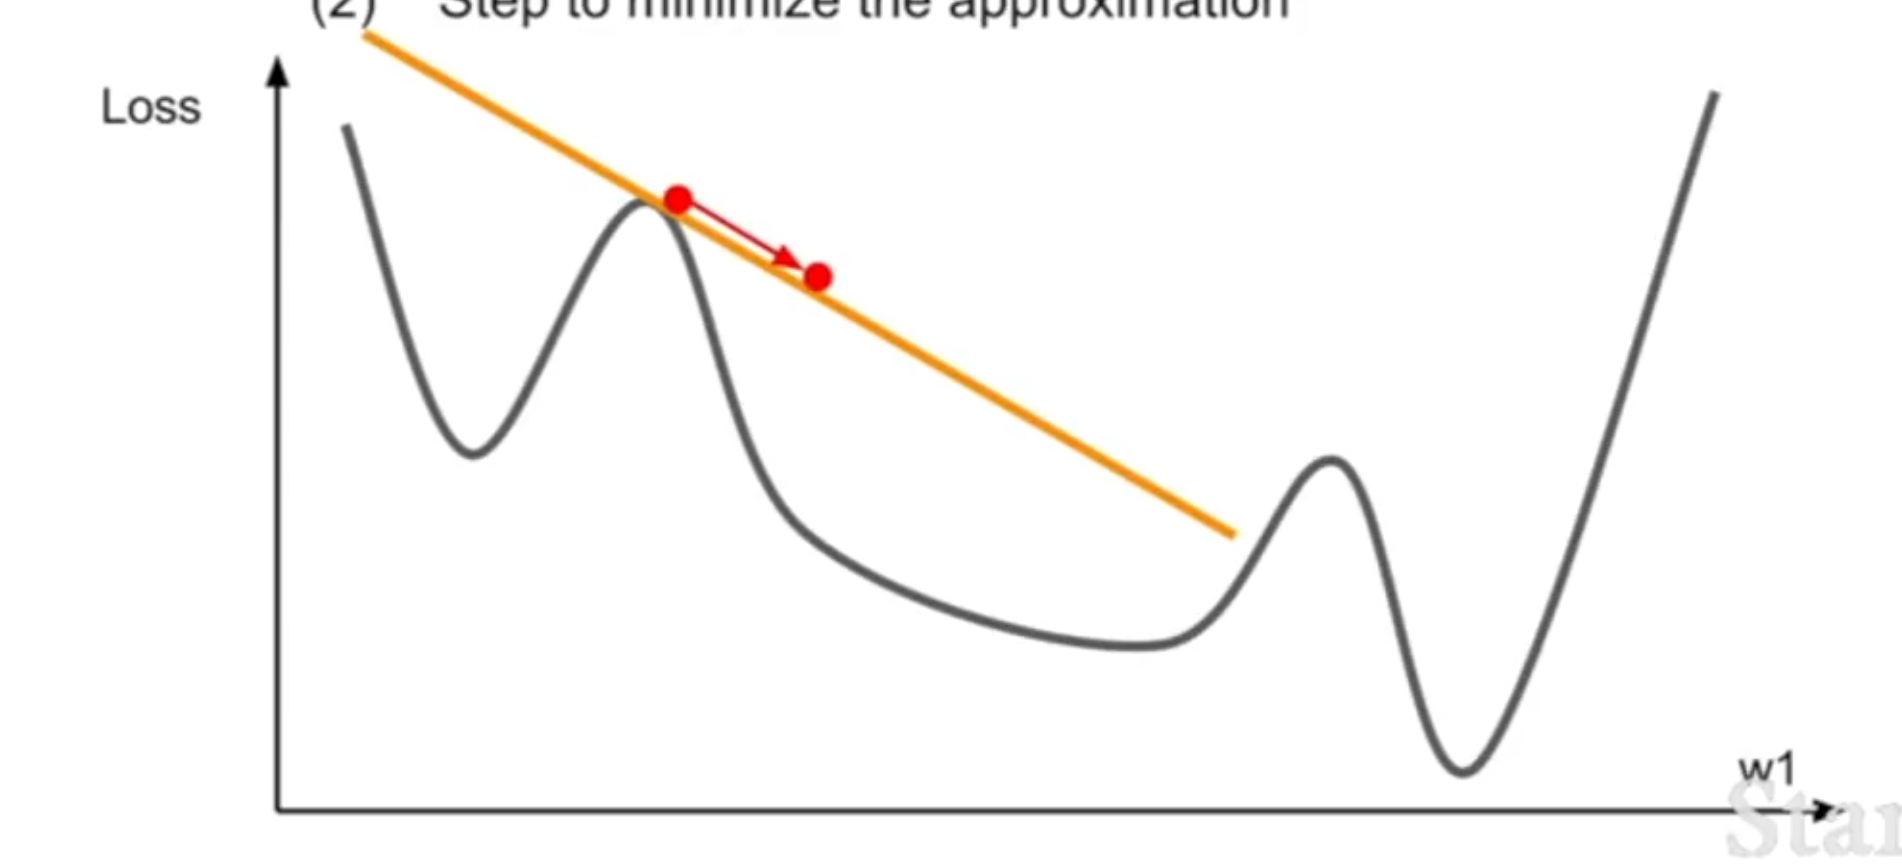
\includegraphics[width=0.5\columnwidth]{fei_fei_li/lecture_07/first_order_approx.png}

\paragraph{Second order approximation}

We can use a second order approx. of the gradient incorporating the Hessian

We can then step to the minimum of the approximated function

This is called the Newton step - it does not have a learning Rate!

This is impractical for deep learning, Hessian is $O(N^2)$ which can be a few millions

cannot invert or store in memory

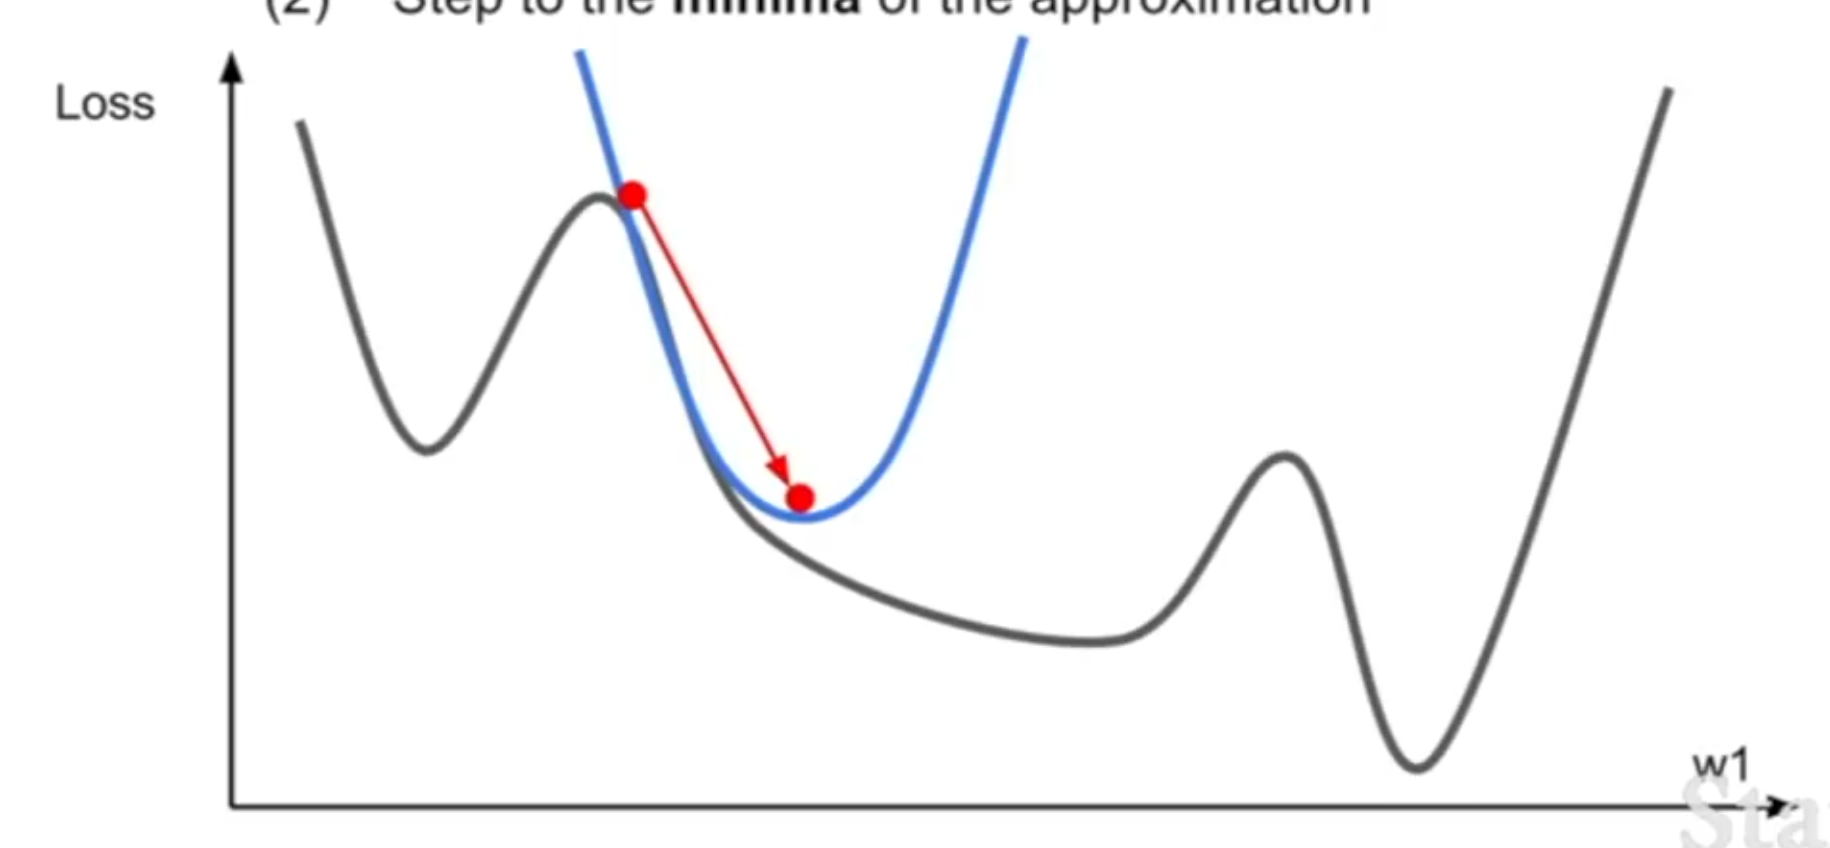
\includegraphics[width=0.5\columnwidth]{fei_fei_li/lecture_07/second_order_approx.png}

Alternative are BFGS and L-BFGS which are approximations of the Hessian

L-BFGS works well for full batch deterministic 

Doesn't work very well for mini-batches, the approximations do not handle the stochastic case too well. In practice counter this by:

- Adam
- If you can afford full batch, LBFGS

Until now all of this was about training error. But we can more about test data, and reducing the gap on test data! So, what can we do? 

\paragraph{Model Ensemble}

1. Train multiple independent models
2. Test time average their results - 2% extra performance
3. Consistent improvement - used often in benchmarks
4. Also keep snapshots of the model during training
5. Polyak averaging - save some running average of the model parameters

\subsubsection{Regularization}

Regularize the model to have it generalize better from training to test data

L2 Regularization - $R(W) = \sum_k\sum_lW_{k,l}^2 $

L1 Regularization - $R(W) = \sum_k\sum_l | W_{k,l} |$

Elastic net - $R(W) = \sum_k \sum_l \beta W^2_{k,l} + | W_{k,l} |$

In practice this regularization doesn't make  too much sense in NN.

\paragraph{	Dropout }

At every forward pass through the network, randomly set some neurons to 0

The probability is a hyper-parameter, usually set to 0.5

More common for fully connected layers, but sometime to might drop channels in conv layers

Dropout means  the network cannot rely on a single feature too much

Similar to doing a model ensemble within a single model

Dropout affects the expected value of our variable - (i didn't get  the full idea of this and it is used in test time) - but at test time we multiply by the dropout probability

For a single neuron with two inputs:

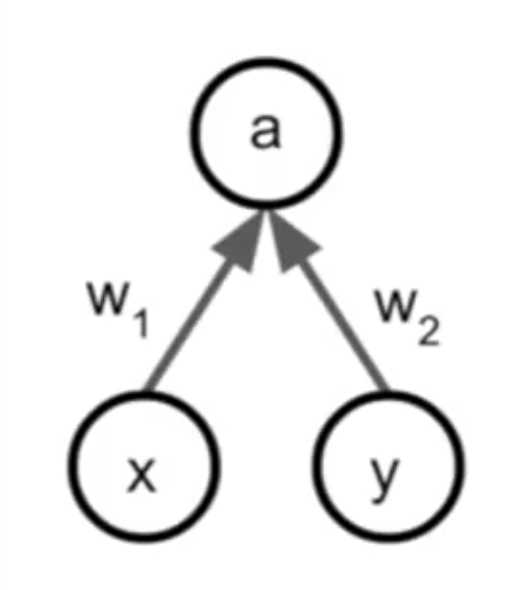
\includegraphics[width=0.5\columnwidth]{fei_fei_li/lecture_07/Screenshot 2019-10-21 at 11.32.00.png}

Train: $E[a] = \frac{1}{4}(w_1x+w_2y)+\frac{1}{4}(w_1x+0y)+\frac{1}{4}(0w_1x+w_2y)+\frac{1}{4}(0x+0y) = \frac{1}{2}(w_1x+w_2y)$

Test: $E[a] = w_1x+w_2y$

At test time - multiply by dropout probability

\paragraph{Inverted Dropout}

You divide by $p$ during training time, rather than multiply by $p$ during test time

Training with dropout takes longer to train, but better generalization after in converged.

A different look at this: 

Training - add randomness

Test - average out randomness

Batch normalization is similar - stochastic relative to a single data point

But dropout gives you control on the amount of randomness vs. batch normalization

\paragraph{Data Augmentation}

- Random image transformation - mirror, cropping
  Resize image at 5 scales
  Report performance at a single crop and at five standard crops

- Color jittering
  Possible in some data dependent way

- Basically - how we can change the data without the label

\paragraph{Drop Connect}

Randomly 0 out the weights

\paragraph{Fractional Max Pooling}

Randomize the regions over which we pool

\subsubsection{Transfer Learning}

For example, want to use learning from a general network to a more specific network which can label 10 dog breeds from a smaller dataset

Cafe etc are 

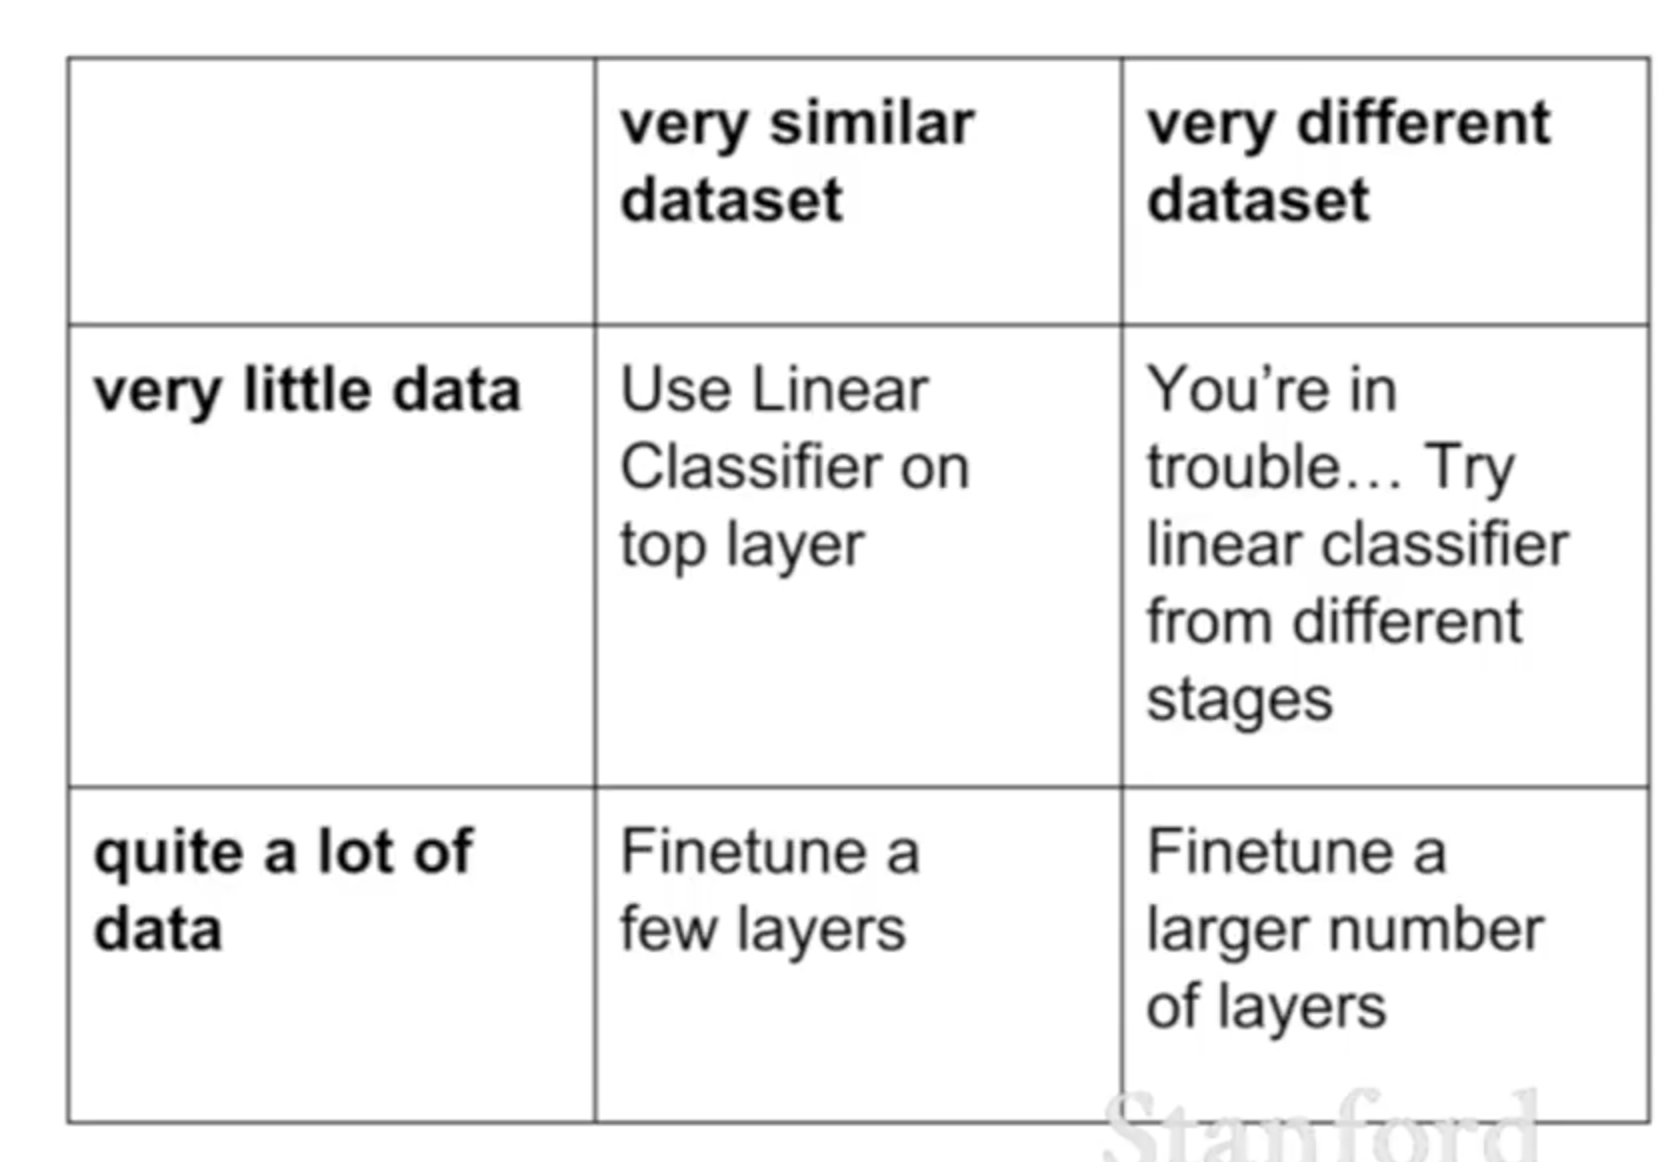
\includegraphics[width=0.5\columnwidth]{fei_fei_li/lecture_07/guidelines_transfer_learning.png}

\subsection{Deep Learning Software}

\subsubsection{CPU vs. GPU}

GPU cores have 3840 units vs. 20 threads running on CPUs 

But they run at lower clock speed, simpler operations

Parallelize one task across many cores

Good for performing a similar task

GPU CPU communication is a bottle neck

12GB memory is the max atm (2017) on GPU memory + caching hierarchy

Matrix multiplications are very suitable on GPU

Benchmarks show 60-70x performance gain

x3 performance gain by using optimized CUDA implementations - use cuDNN

Another problem - model is on GPU and the data is on SSD

this adds a bottle neck - solutions:

	- read data in RAM
	- use SSD
	- multiple CPU threads to pre-fetch data
	- 

\subsubsection{TensorFlow}

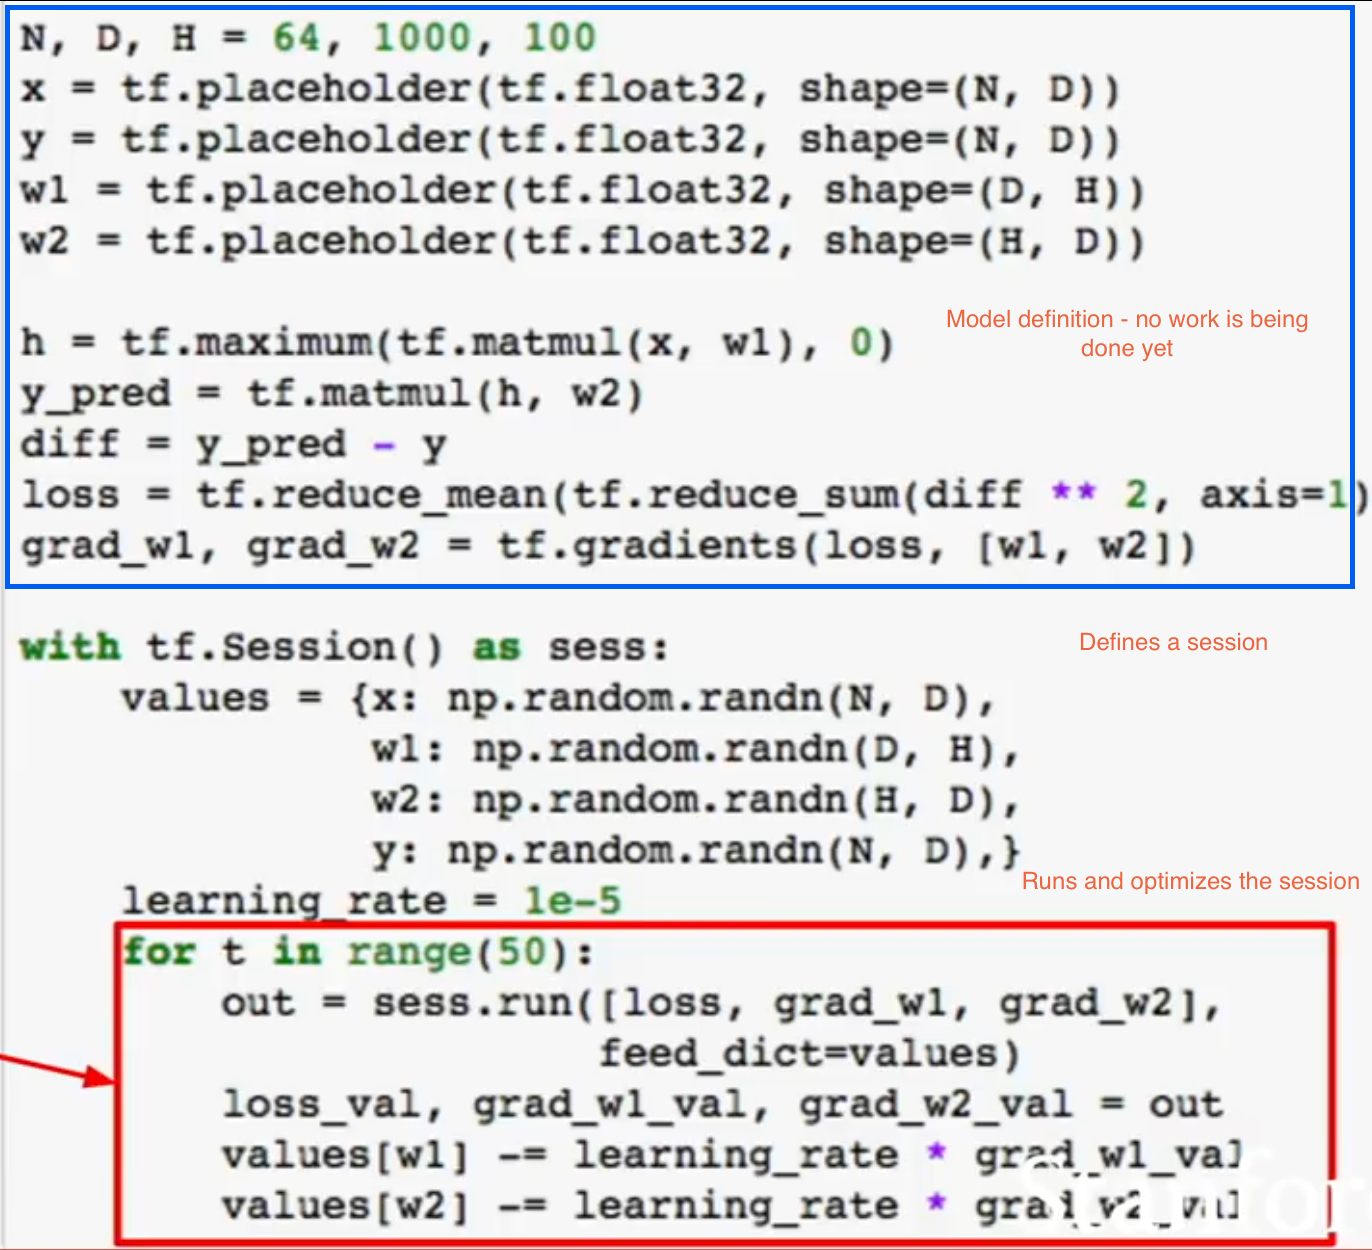
\includegraphics[width=0.5\columnwidth]{fei_fei_li/lecture_08/Screenshot 2019-10-21 at 12.32.42.png}

Where it's done like this - every time we run the graph we're copying the weights from numpy arrays to memory, etc. very expensive.

The solution is to setup w1 and w2 as tf.Variable - lives inside the computational graph and we also need to tell TF how to initialize them

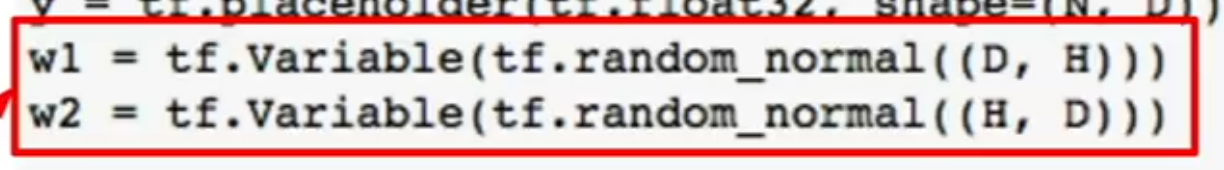
\includegraphics[width=0.5\columnwidth]{"fei_fei_li/lecture_08/Screenshot 2019-10-21 at 12.45.00.png"}

So in this version the weights update step needs to live within the computational graph, so the final version is this? 

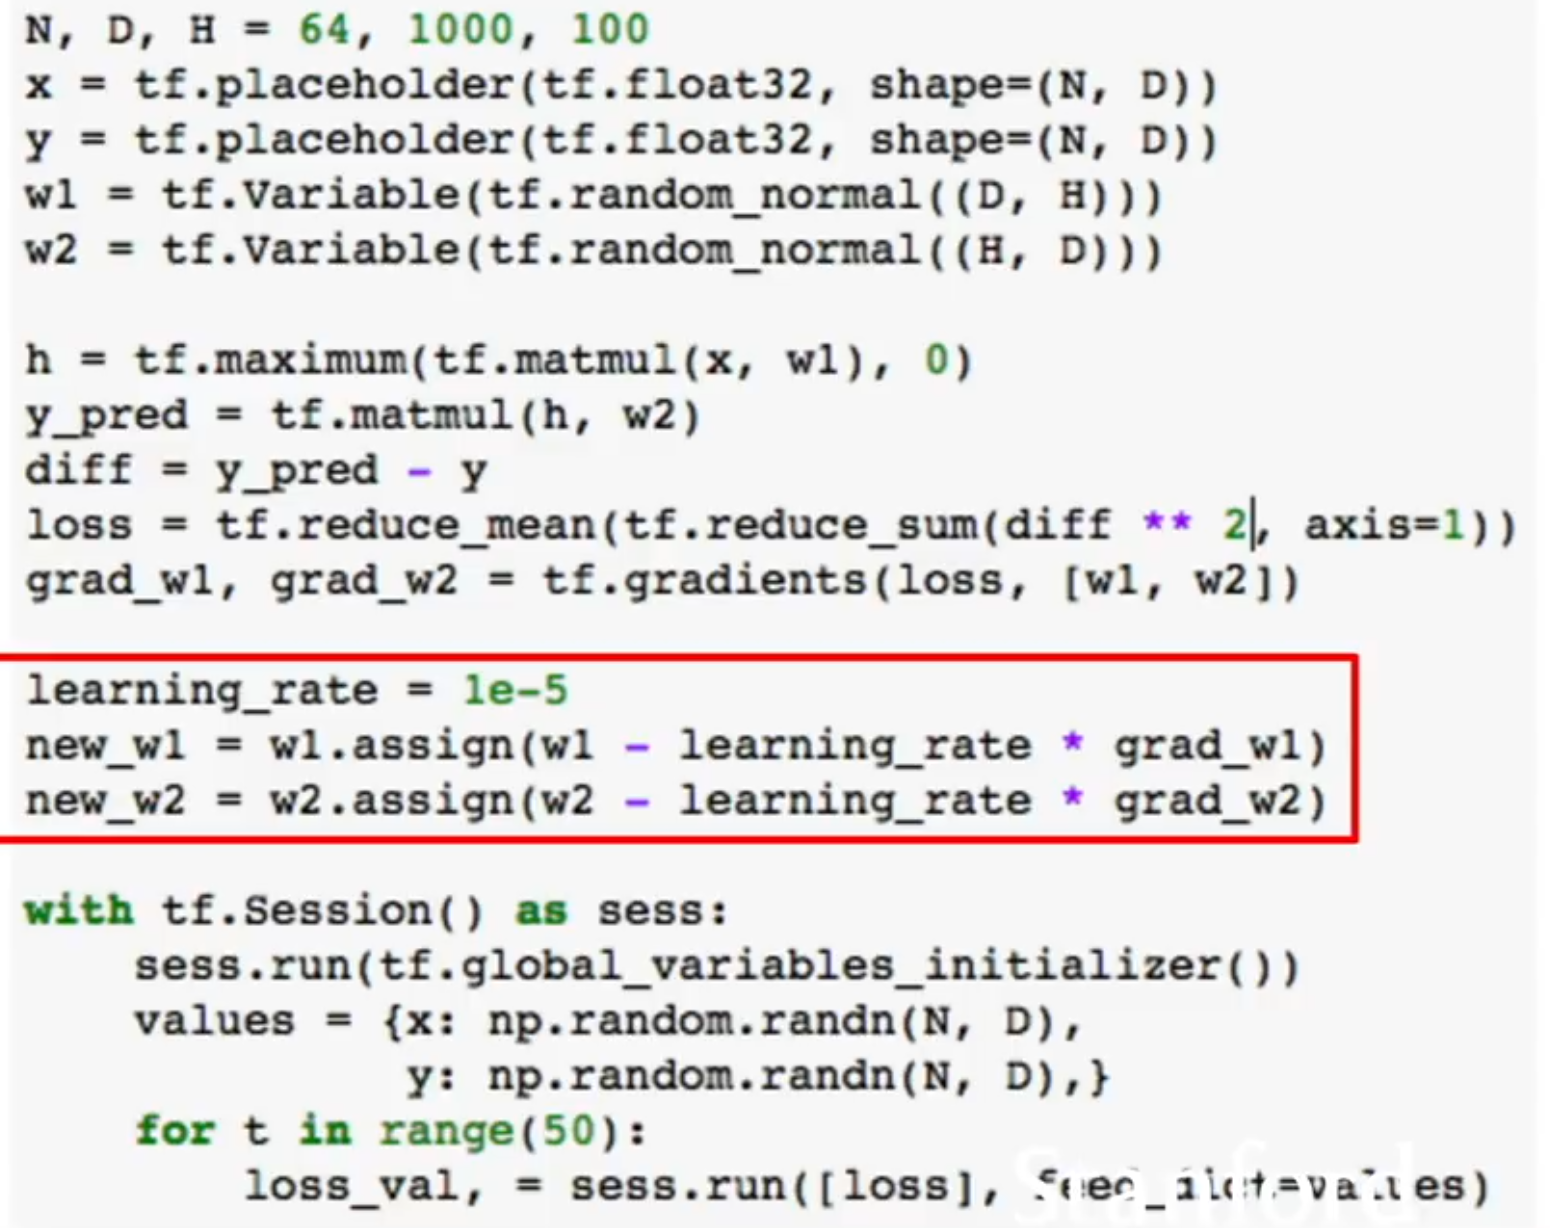
\includegraphics[width=0.5\columnwidth]{fei_fei_li/lecture_08/tf_in_memory.png}

so we have to add a dummy node which is responsible for updating the weights:

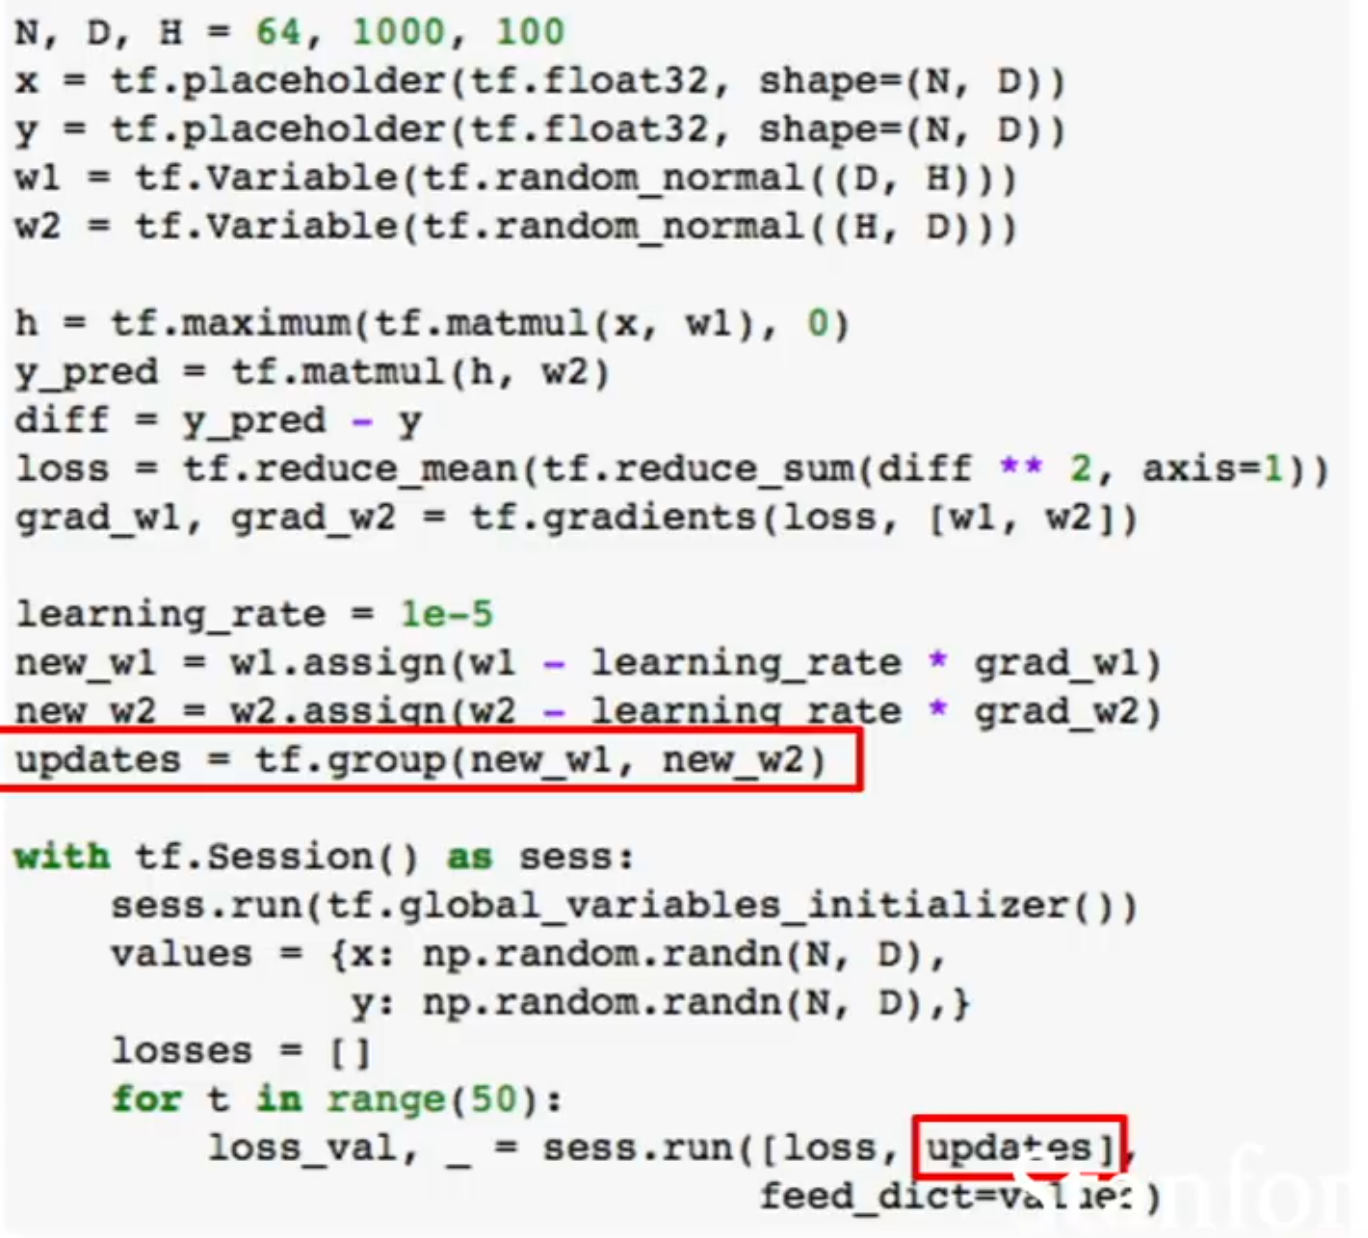
\includegraphics[width=0.5\columnwidth]{fei_fei_li/lecture_08/tf_memory_updates.png}

and tell tf to update the node.

This is a bit ugly, we can simple use an TF optimizer: 

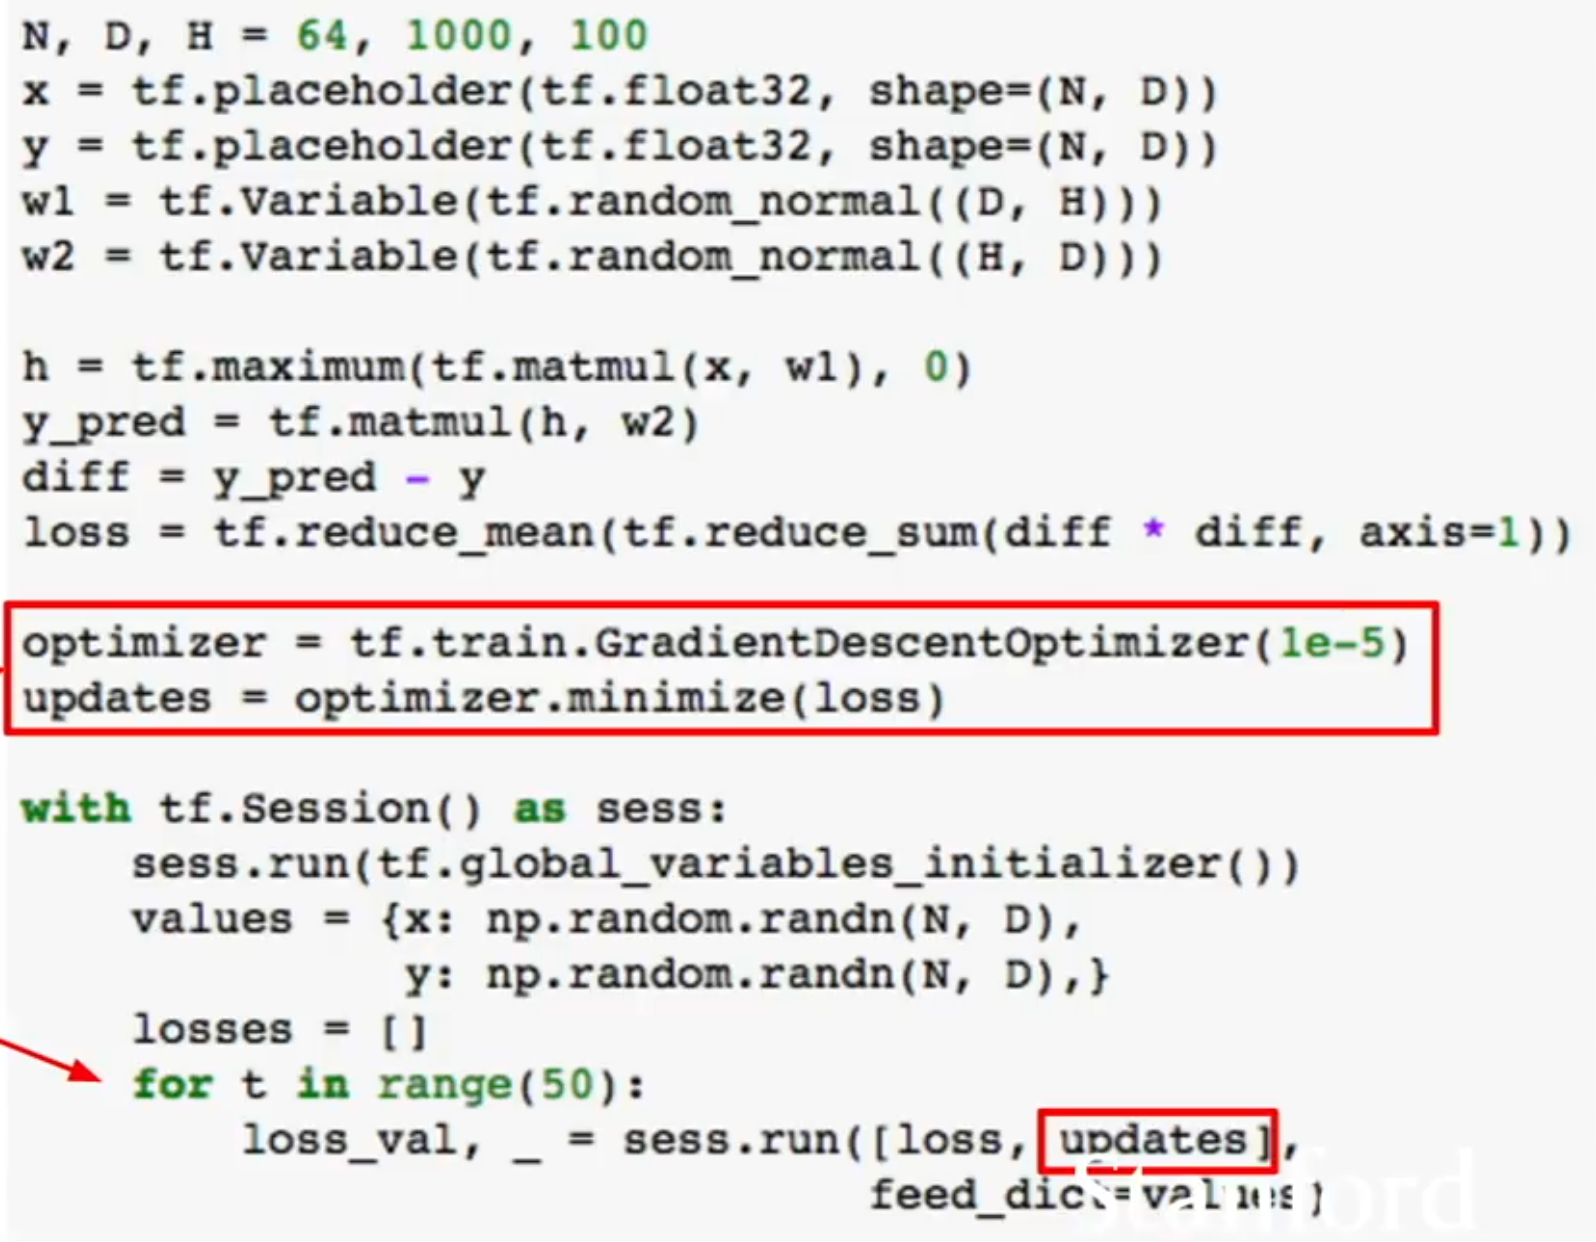
\includegraphics[width=0.5\columnwidth]{fei_fei_li/lecture_08/optimizer.png}

which adds the relevant nodes to the graph (compute gradients, update weight, group operations)

\subsubsection{PyTorch}

Has 3 different levels of abstraction

- tensor - imperative ndarray on gpu
- variable - node in a comp. graph
  - support automatic diff
  - same API as tensors
  - flagged if we want to compute gradients
- module - nn layer, may store state and learnable weights



\paragraph{tensors}

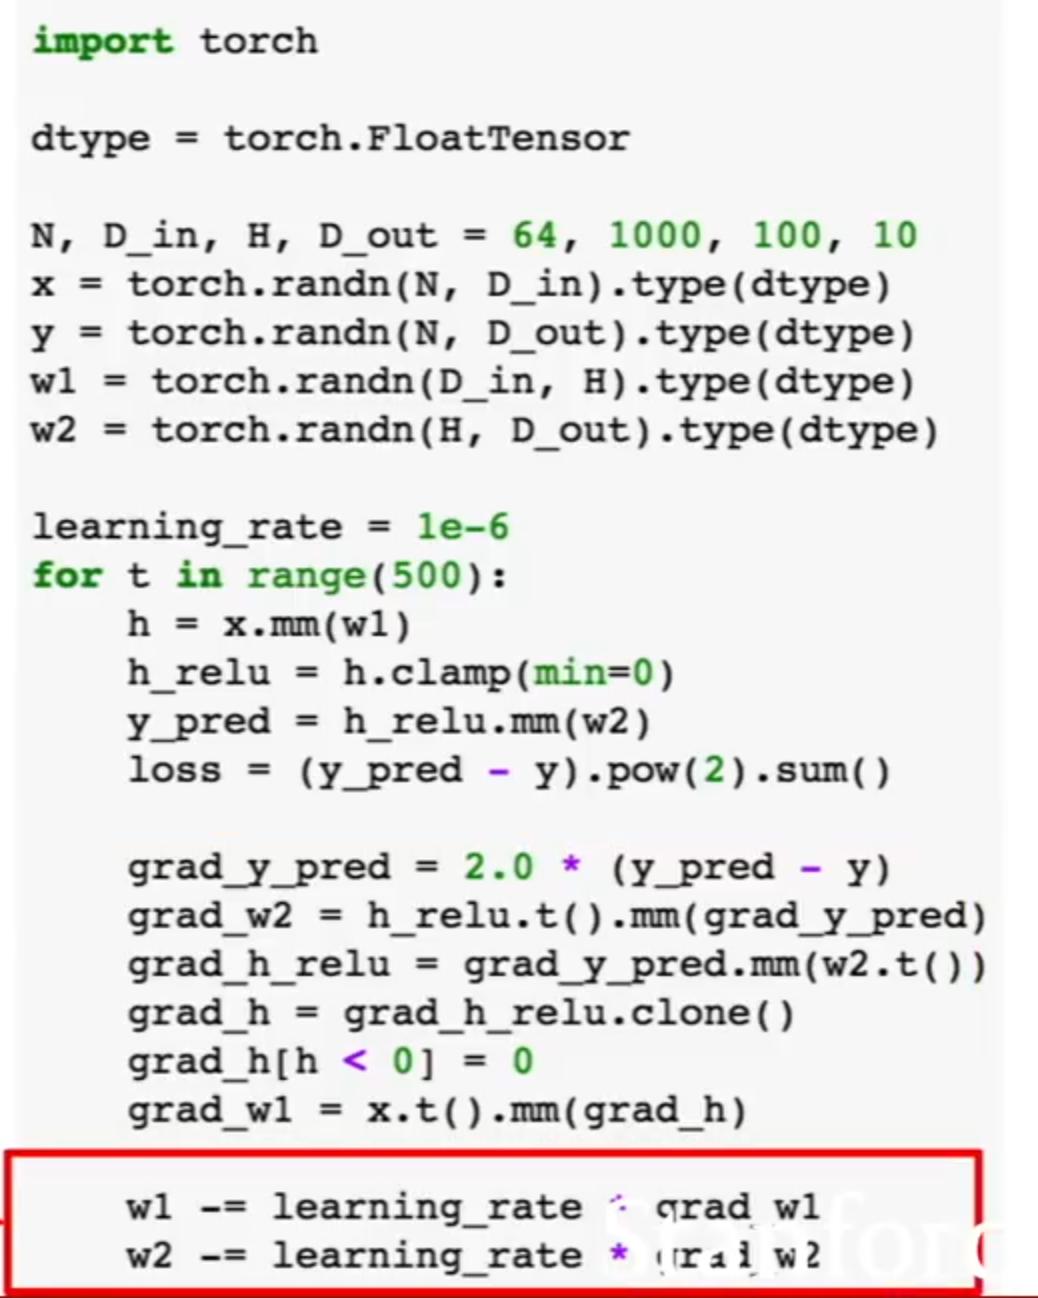
\includegraphics[width=0.5\columnwidth]{fei_fei_li/lecture_08/pytorch_tensors.png}

\paragraph{Variables + autograd}

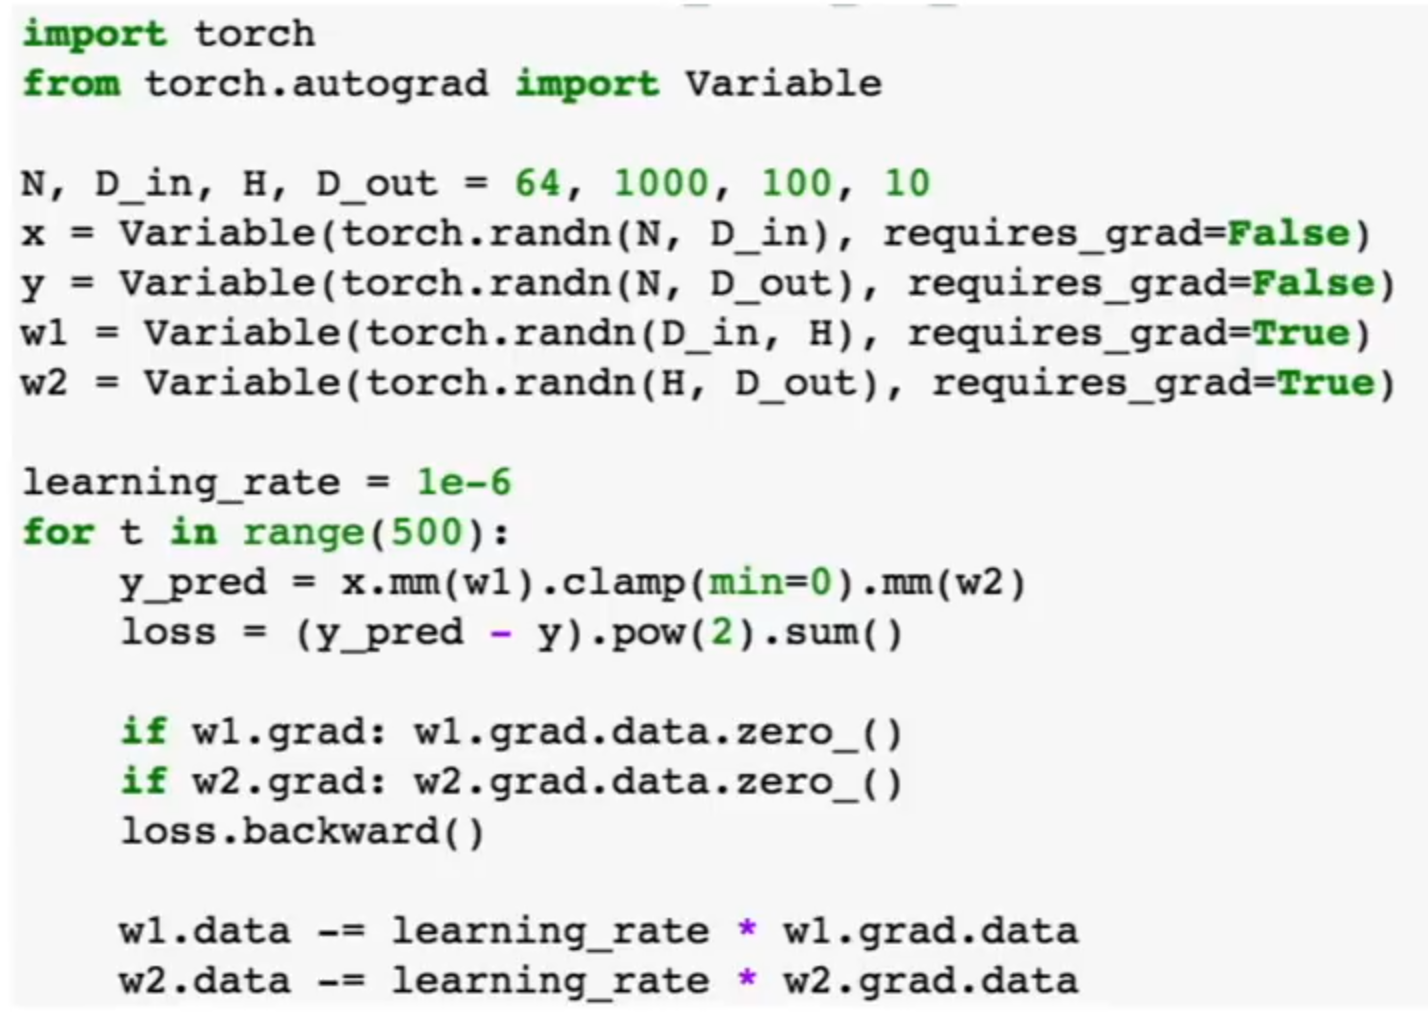
\includegraphics[width=0.5\columnwidth]{fei_fei_li/lecture_08/pytoch_variable.png}

- PyTorch we build a new graph at every forward pass which makes the code a bit cleaner
- Define autograd functions by writing forward and backwards func. imp. for Tensors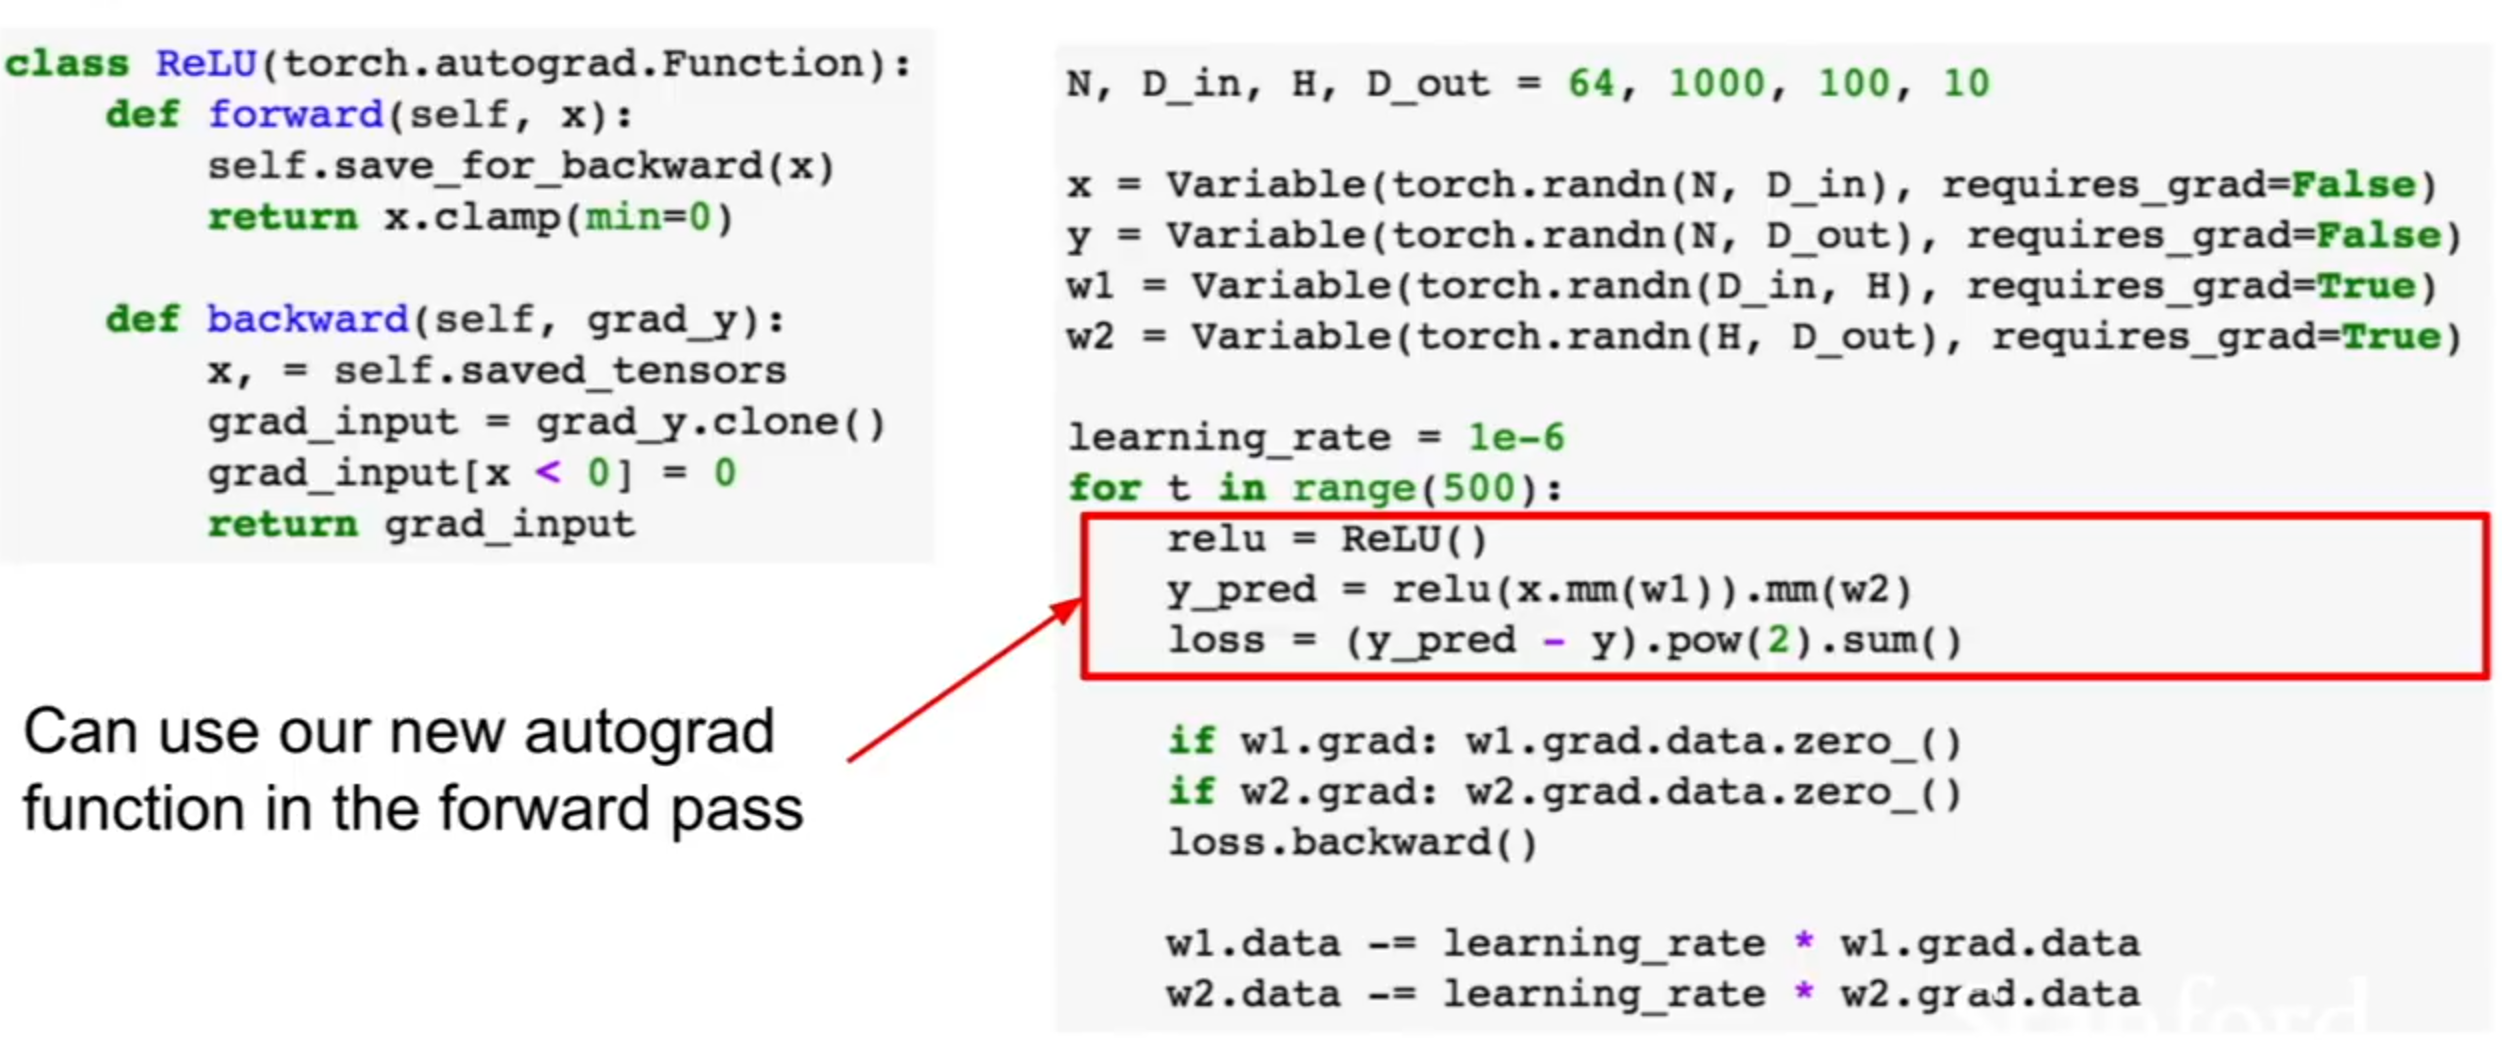
\includegraphics[width=0.5\columnwidth]{fei_fei_li/lecture_08/pytorch_autograd.png}
- we also work at the higher level:
- 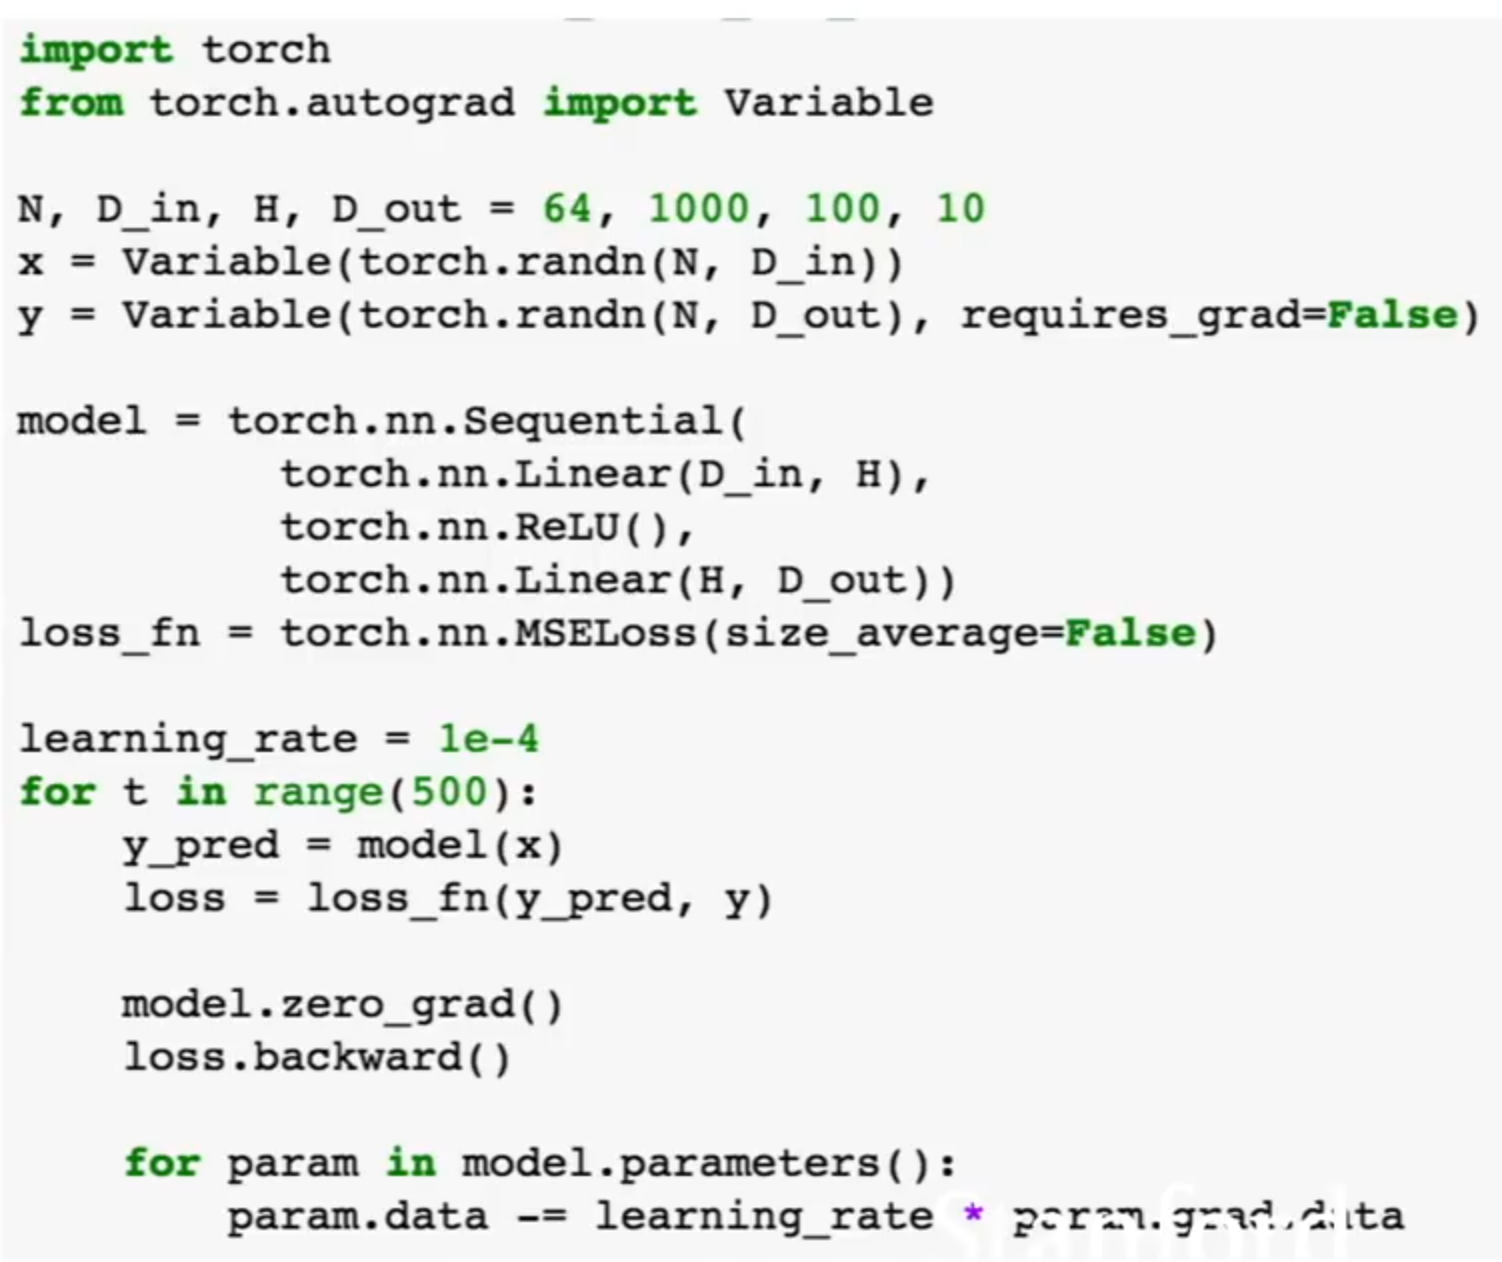
\includegraphics[width=0.5\columnwidth]{fei_fei_li/lecture_08/pytorch_nn.png}



Modules



\paragraph{DataLoader }

write a data class that knows how to load and prepare the data



\paragraph{Complete PyTorch Pipeline}

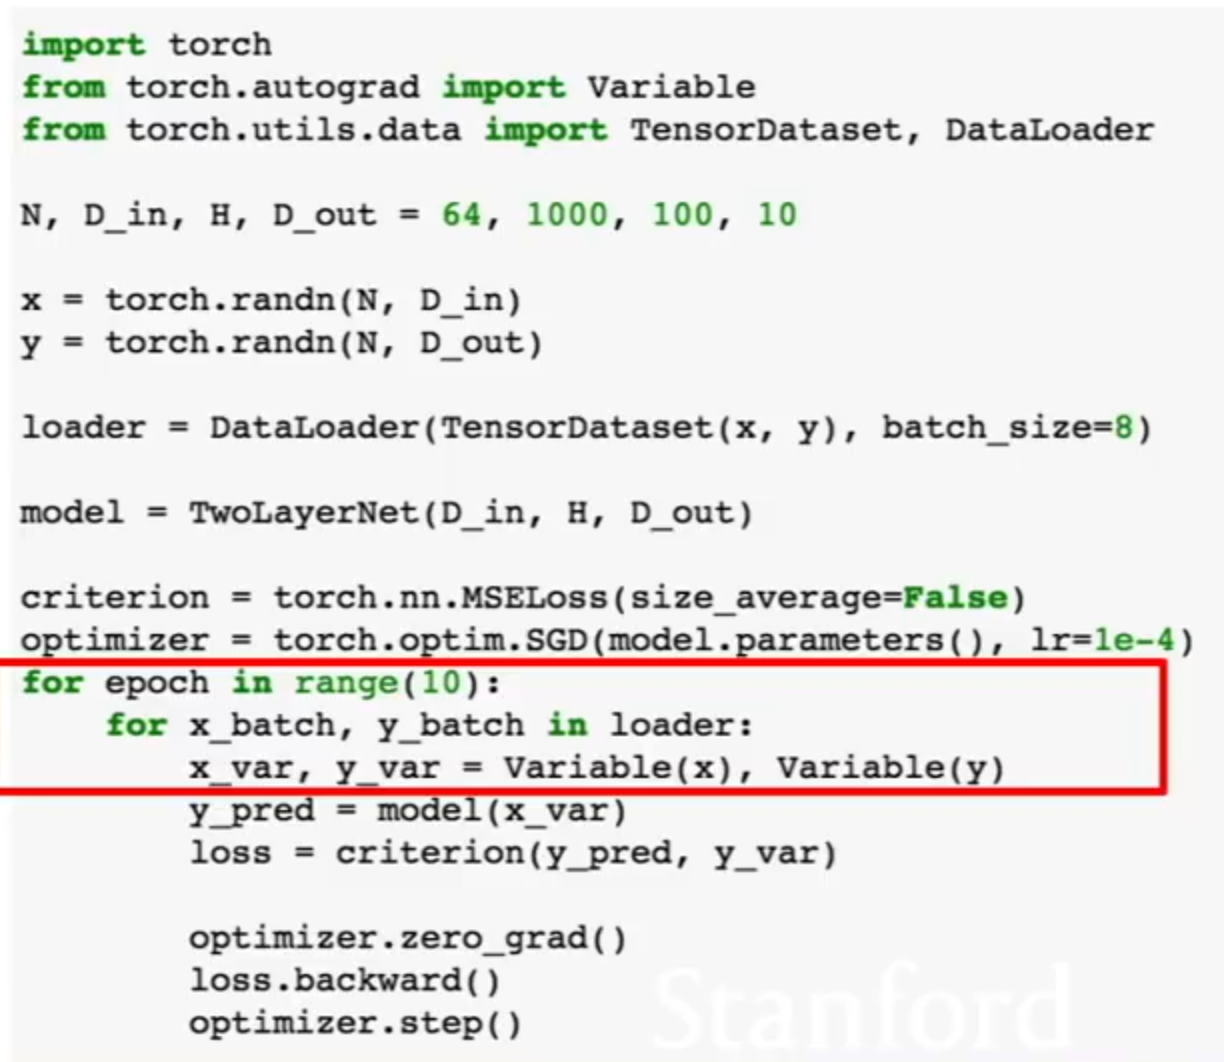
\includegraphics[width=0.5\columnwidth]{fei_fei_li/lecture_08/complete_pytorch_pipeline.png}

\subsubsection{Static vs. Dynamic Graphs}

TensorFlow - build once, run many times (static)

PyTorch - re-built at every run (dynamic)

For simple network, makes no difference

Static case

- network can do simple optimizations on the graph operations
  - more efficient - fused operations
  - more expensive upfront, but amortized over time
- you can serialize the graph and the structure of the network
  - nice for deployment scenario

Dynamic case:
\begin{itemize}
\item conditional operations
\item in tensor flow it's tf.cond() which needs to be baked into the graph
\item loops
\item RNNs is a good motivation for dynamic graphs
\end{itemize}

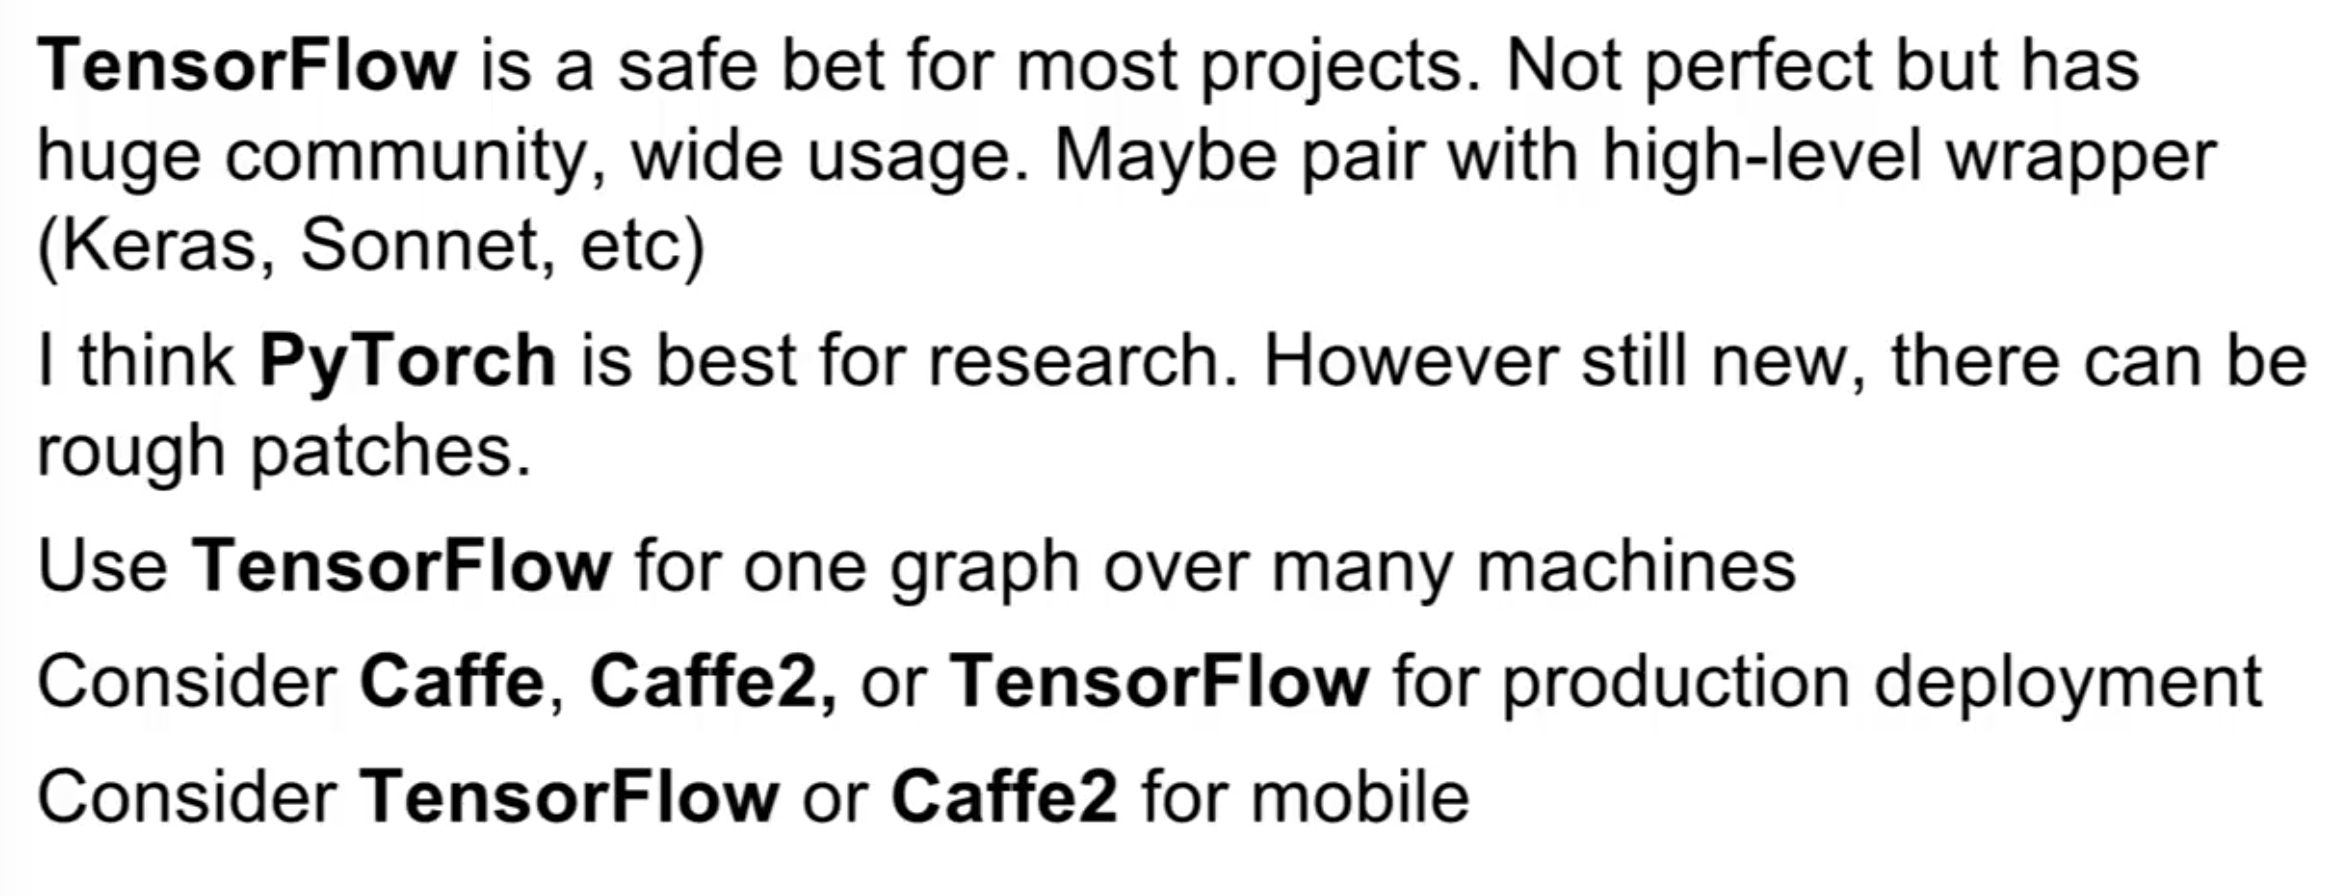
\includegraphics[width=0.5\columnwidth]{fei_fei_li/lecture_08/what_to_use.png}

\subsection{CNN Architectures}
\subsubsection{AlexNet}

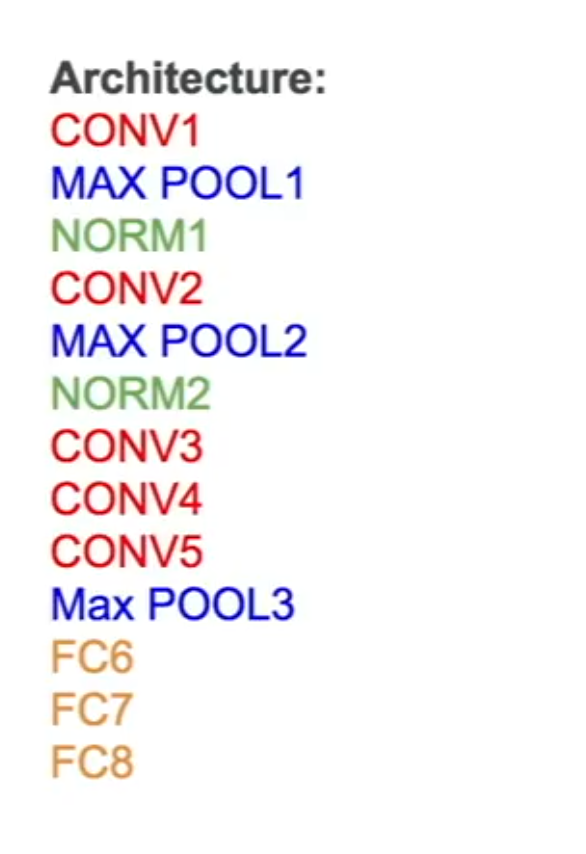
\includegraphics[width=0.25\columnwidth]{fei_fei_li/lecture_09/alex_net_2.png}

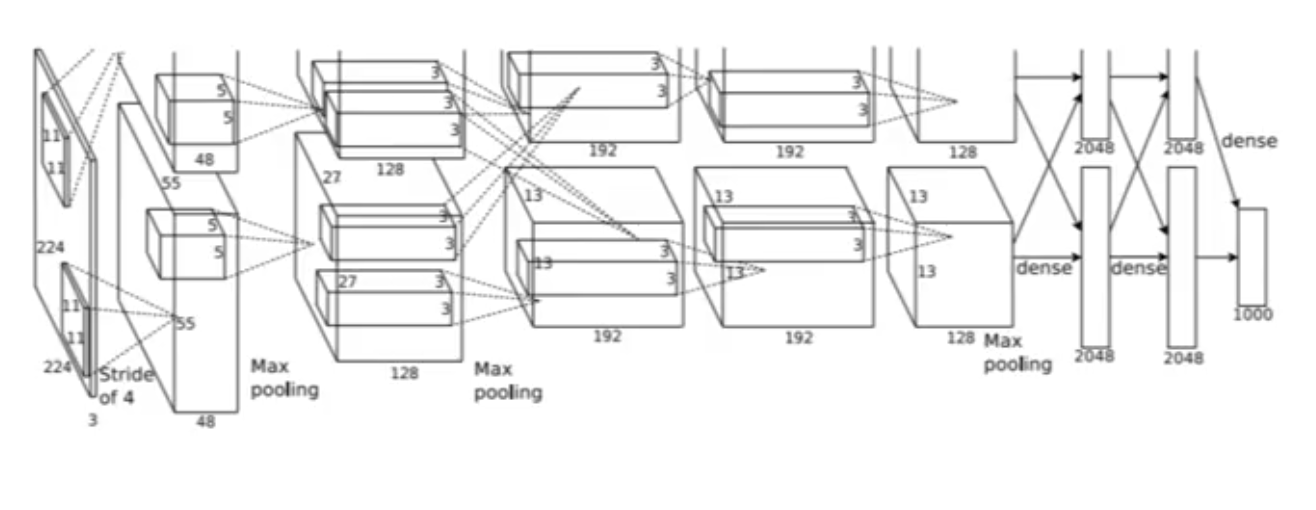
\includegraphics[width=0.5\columnwidth]{fei_fei_li/lecture_09/alex_net.png}

\subsubsection{Introduction of Deeper Networks}
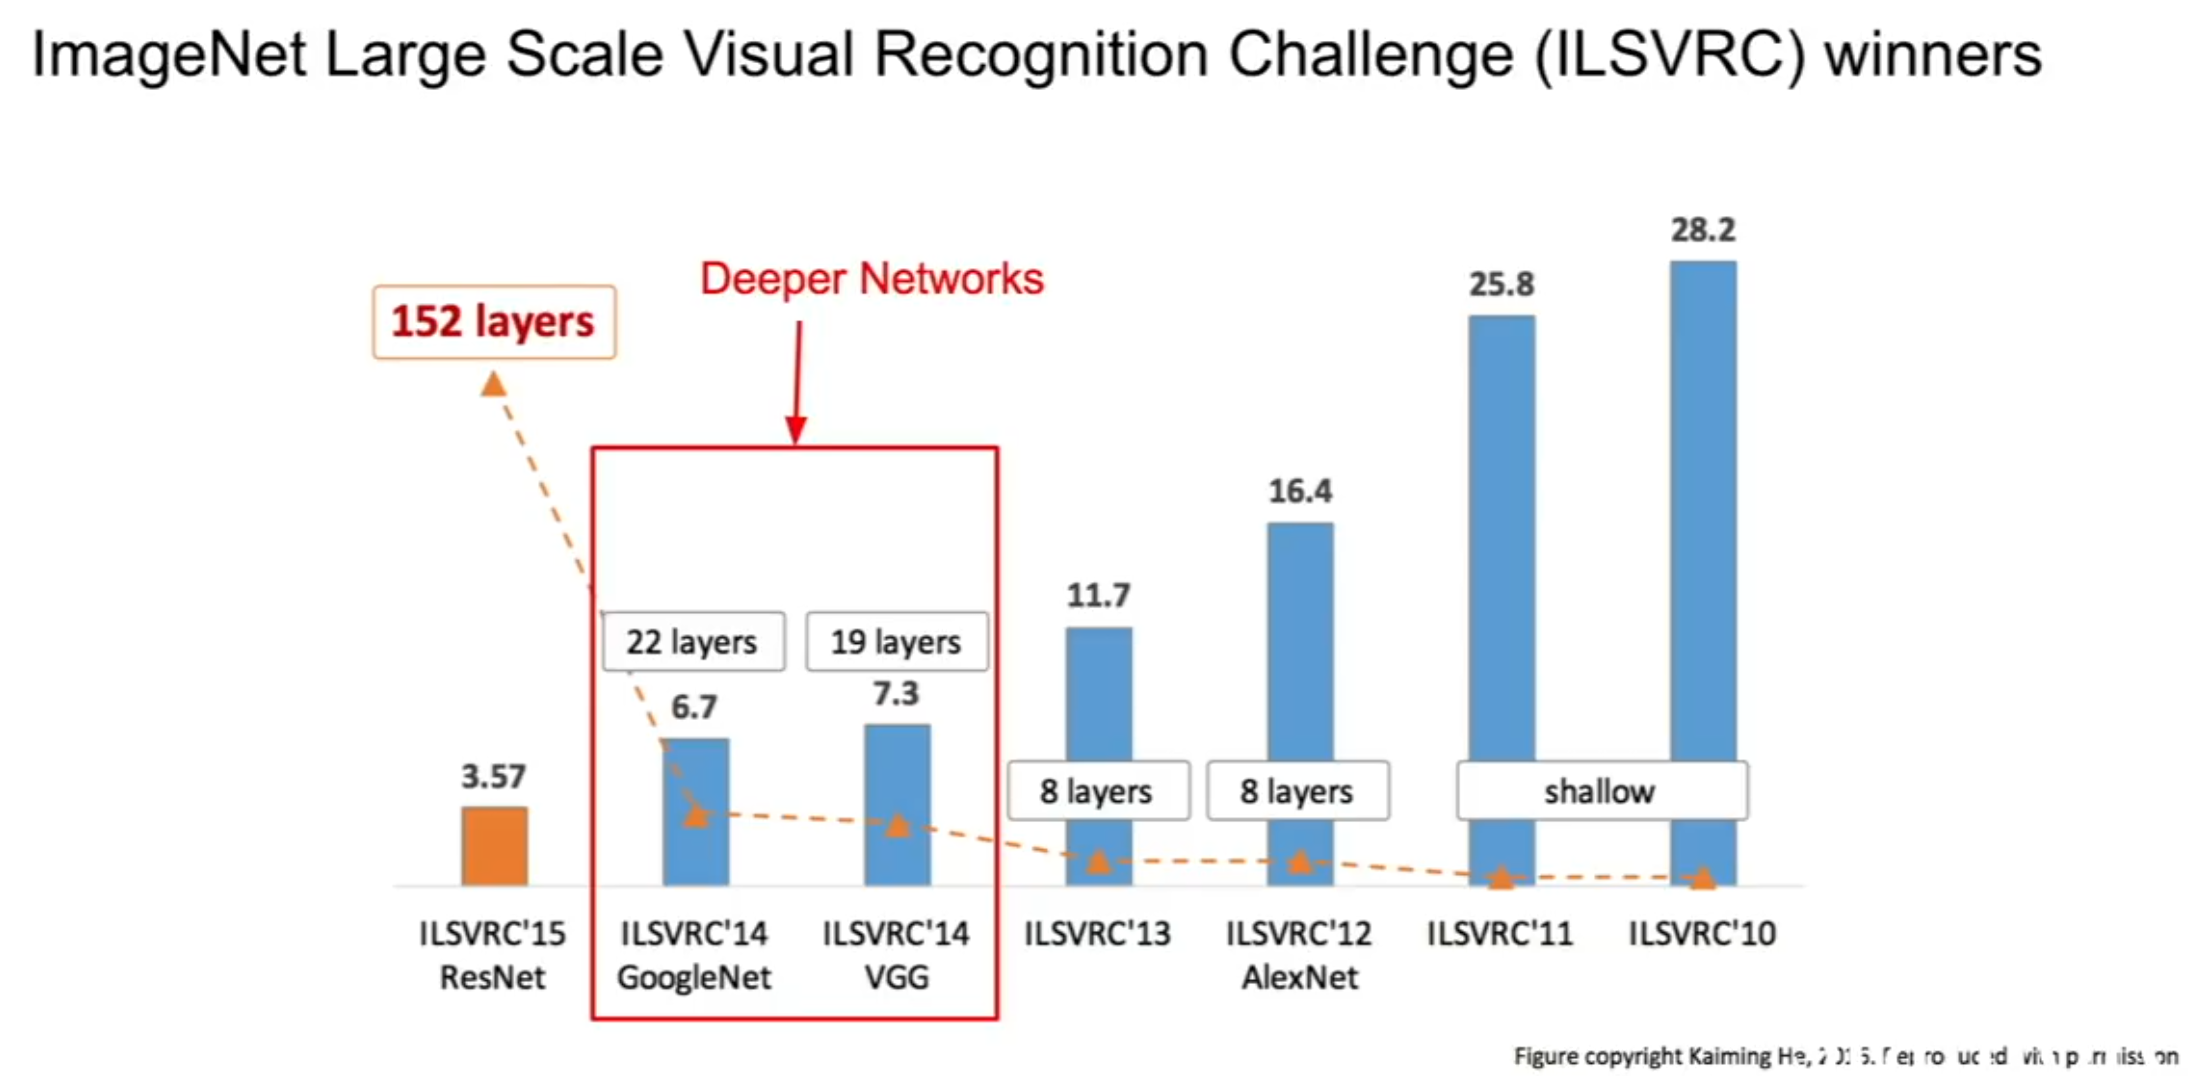
\includegraphics[width=0.5\columnwidth]{fei_fei_li/lecture_09/deeper_networks.png}

\subsubsection{GoogleNet}

- only 5 million params, x12 less than alexnet

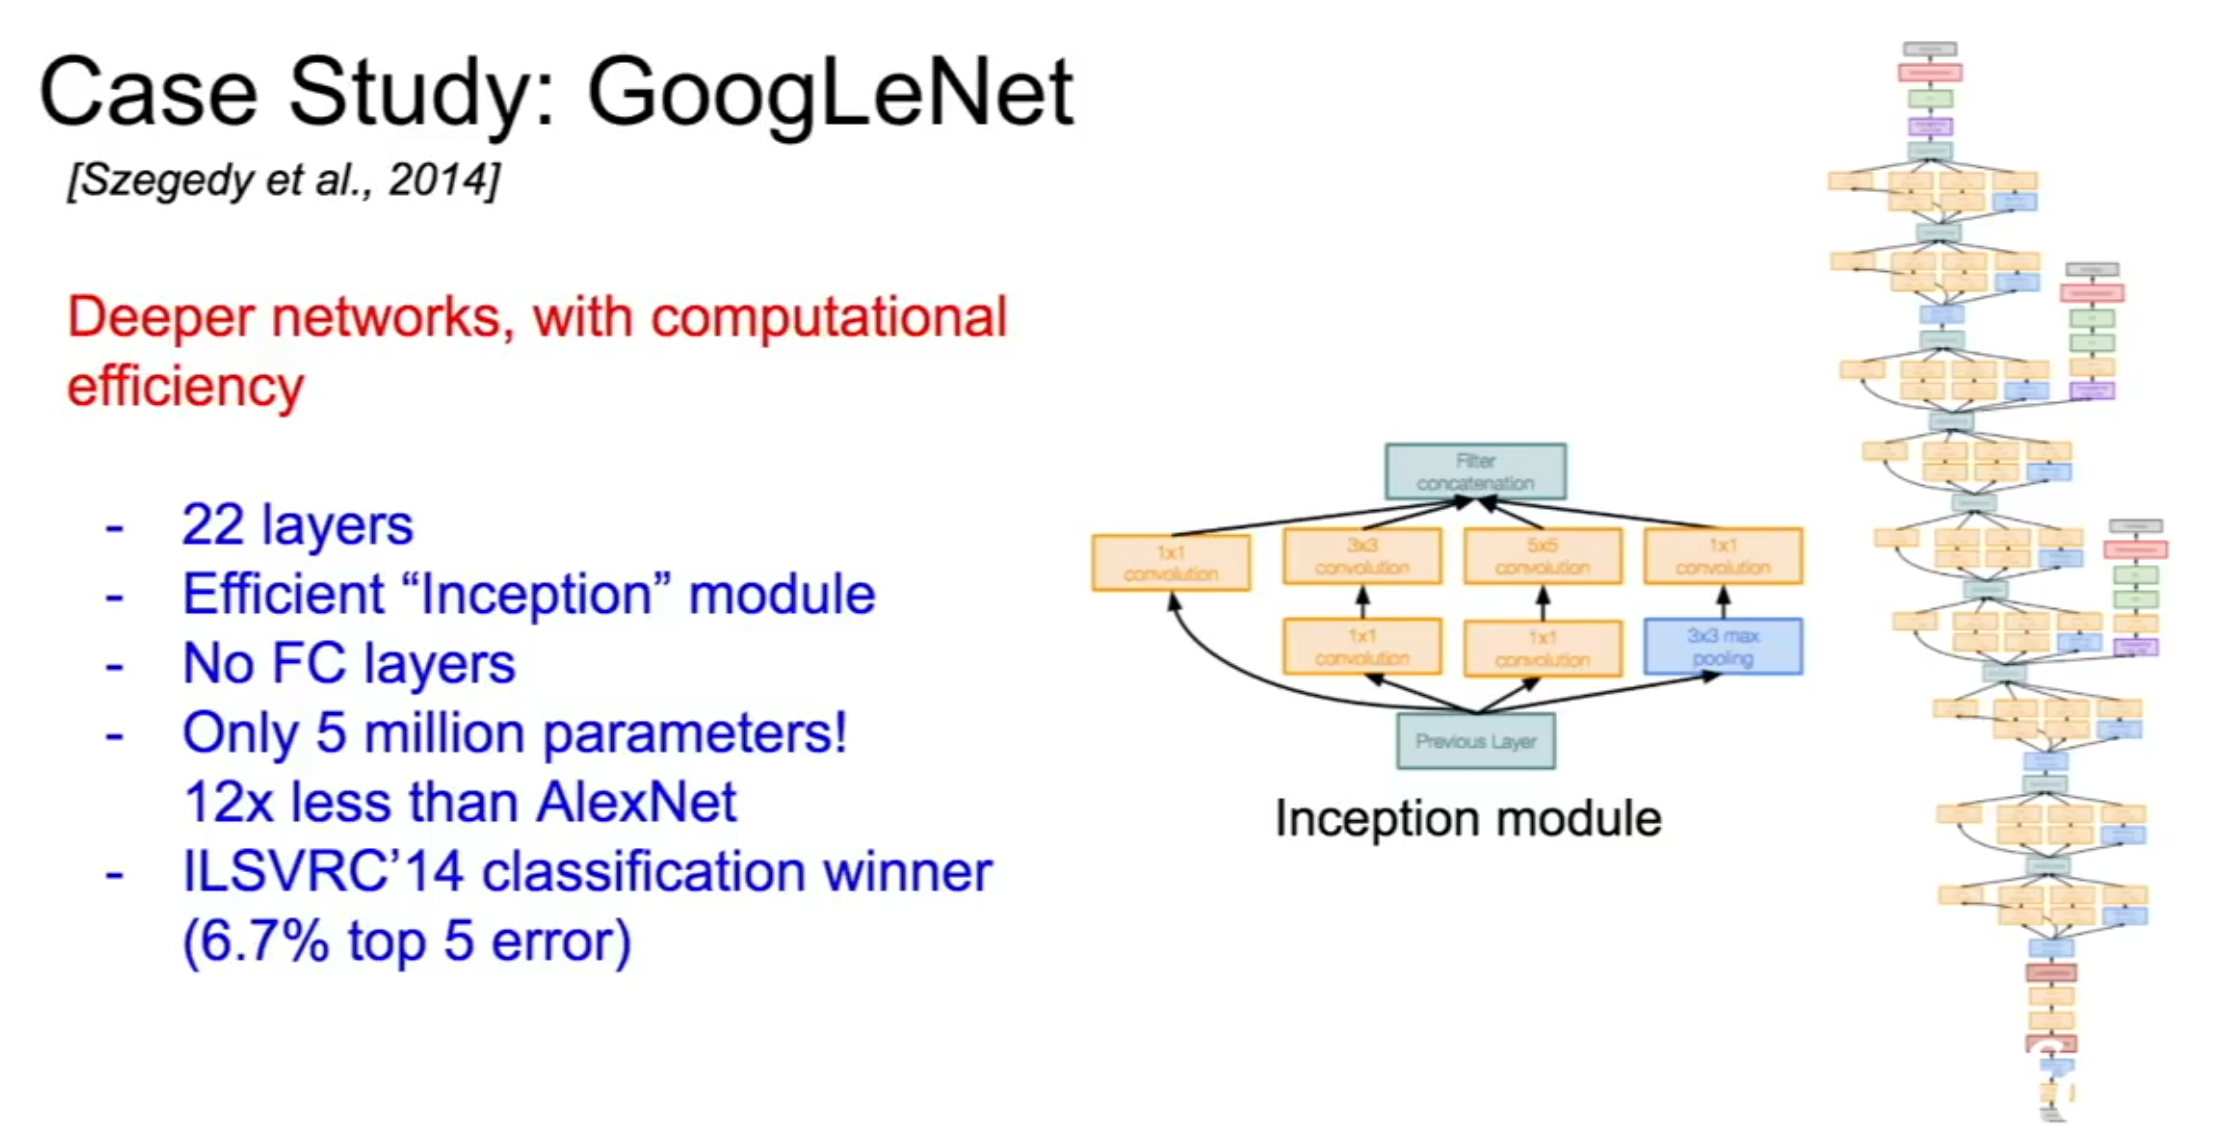
\includegraphics[width=0.5\columnwidth]{fei_fei_li/lecture_09/google_net.png}

\textbf{Inception Module}

Design a good local network topology (network within a network) and stack them together:

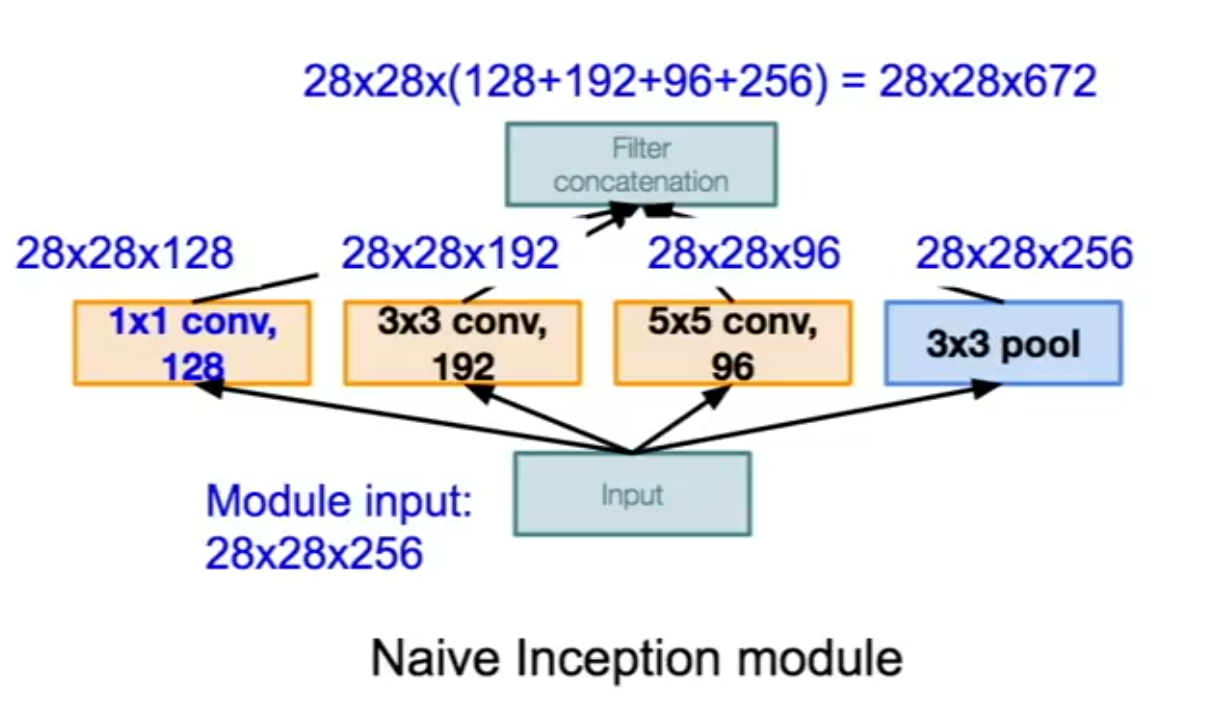
\includegraphics[width=0.5\columnwidth]{fei_fei_li/lecture_09/naive.png}

The idea is to have different operations on the same output, and then concatenate the output of these layers together.

What are the problems with this? 
\begin{itemize}
\item computational complexity - 854 mops
\item output depth - 28x28x672
\end{itemize}

How to keep this manageable?
\begin{itemize}
\item 1x1 conv with 32 filters operating on 56x56x64 $->$ 56x56x32 
\item conv layers preserve spatial information but can reduce depth
\item projecting the input to lower dimension before expensive operations:
\end{itemize}

The optimized version has 358Mops vs. 854

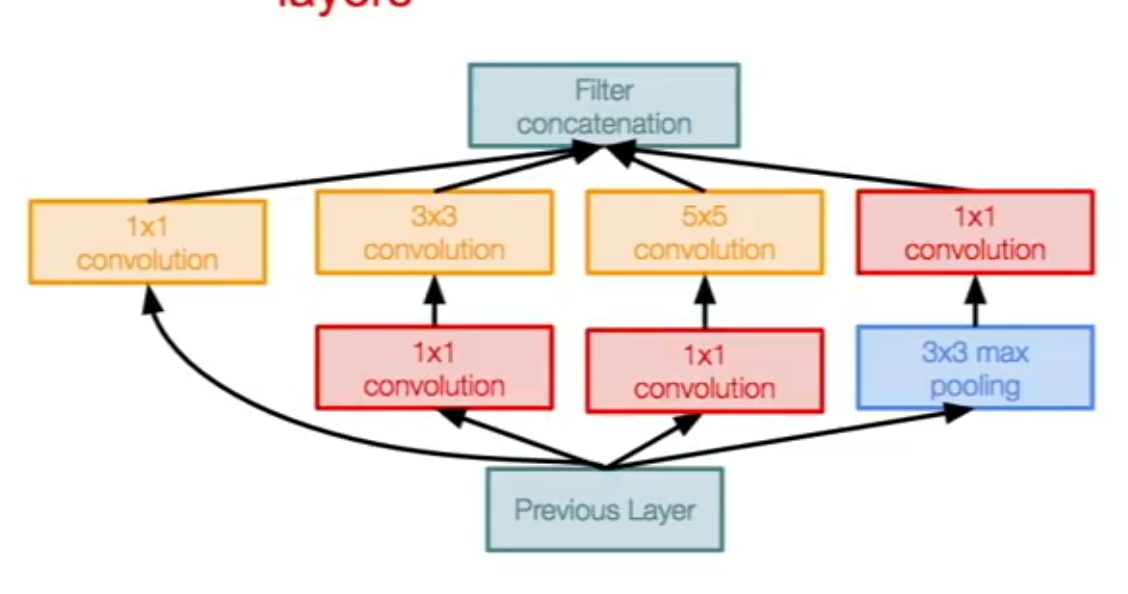
\includegraphics[width=0.5\columnwidth]{fei_fei_li/lecture_09/less_naive.png}

\paragraph{ResNet}

Revolution of depth - 152 resnet architecture

Extremely deep network using residual connections

Why is this special? 

Adding depth to a normal network $\rightarrow$ worse training response

The training error is doing worse - not because of overfitting.

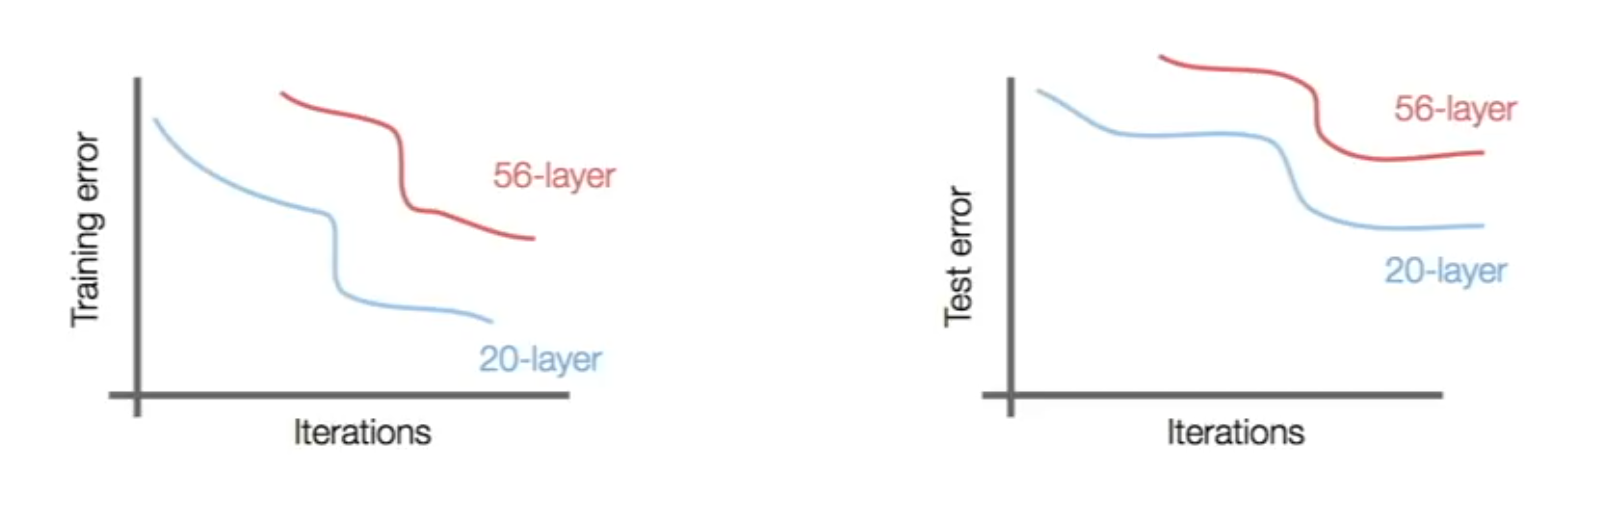
\includegraphics[width=0.5\columnwidth]{fei_fei_li/lecture_09/deep_error.png}

The problem is an optimization problem - harder to optimize

Reasoning - a deeper model should perform just as well a shallower model - for example, train 20 layer model, copy the params, add 20 more layers of identity

$\Rightarrow$ I really do not understand this "residual"

- Were able to train very deep networks without degrading
- Deeper networks can now achieve lower training error - better gradient propagation

\subsubsection{Complexity}

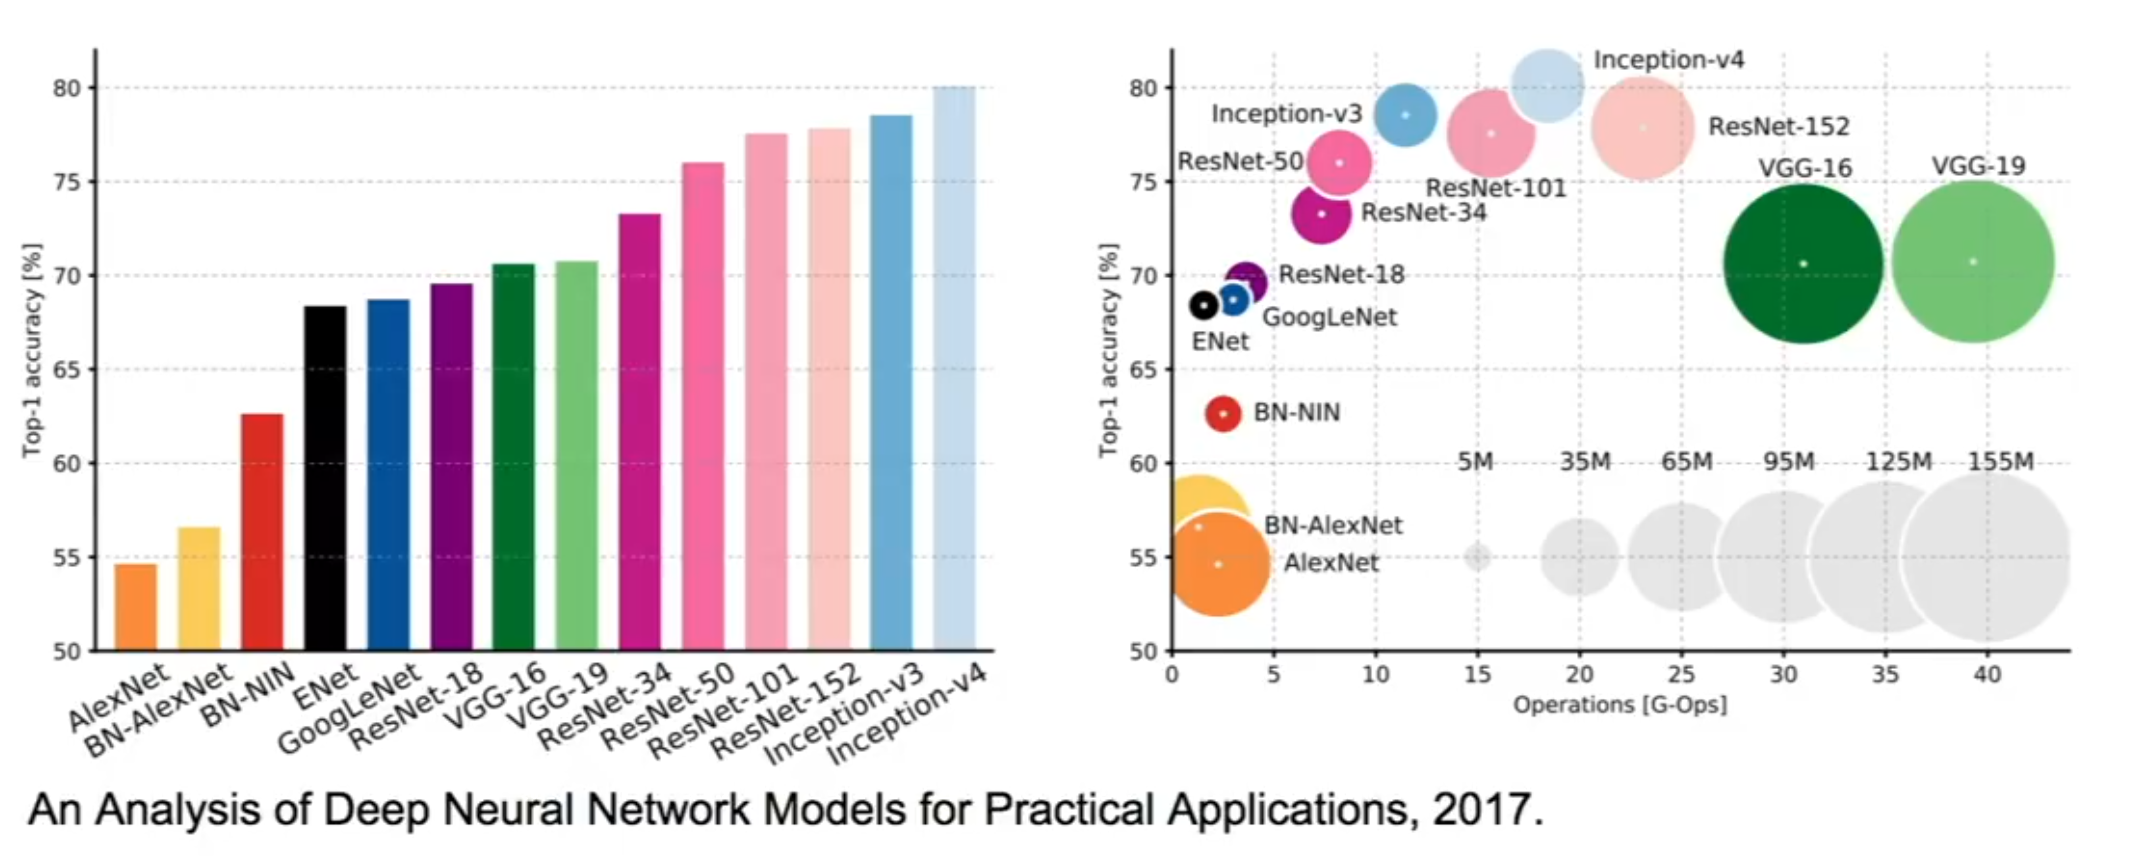
\includegraphics[width=0.5\columnwidth]{fei_fei_li/lecture_09/complexity.png}



Developments on top ResNet: 

- Huang 2016 - Deep Networks with Stochastic Depth
  - reduce vanishing gradients and training time through short network training
  - drop layers randomly at every pass, use identity
  - use full network at test time

Fractal Net

- motivation: transitioning to residual representations are not necessary

Densely Connected Convolutional Networks

Recap of CNN architecture: 

\subsubsection{More Insights of The ResNet Arch}

we pass the input through conv blocks (conv + relu)  and then add the input to the output of these blocks

if the weights are 0 - it's simply identity

interpretation of l2 regularization of the network - encourages the model to drive unneeded layers

Gradient flow in backward pass:

- addition gradient will stream and fork along two different paths
- upstream gradient will have direct connection - gradient super highway

Also DenseNet and FractalNet allow for easy gradient pass through the network



\subsubsection{More Insight on Architectures }

AlexNet and VGG have a lot of params in fully connected layers

\textbf{AlexNet}

- ~62M params -> out of which most live in a few layers:
  -  FC6 256x6x6 -> 4096: 38M Params
  - FC7 4096 -> 4096: 17M Params
  - FC7 4096 -> 1000: 4M Params
  - 59M params in 3 layers

\subsection{Recurrent Neutral Network }

% 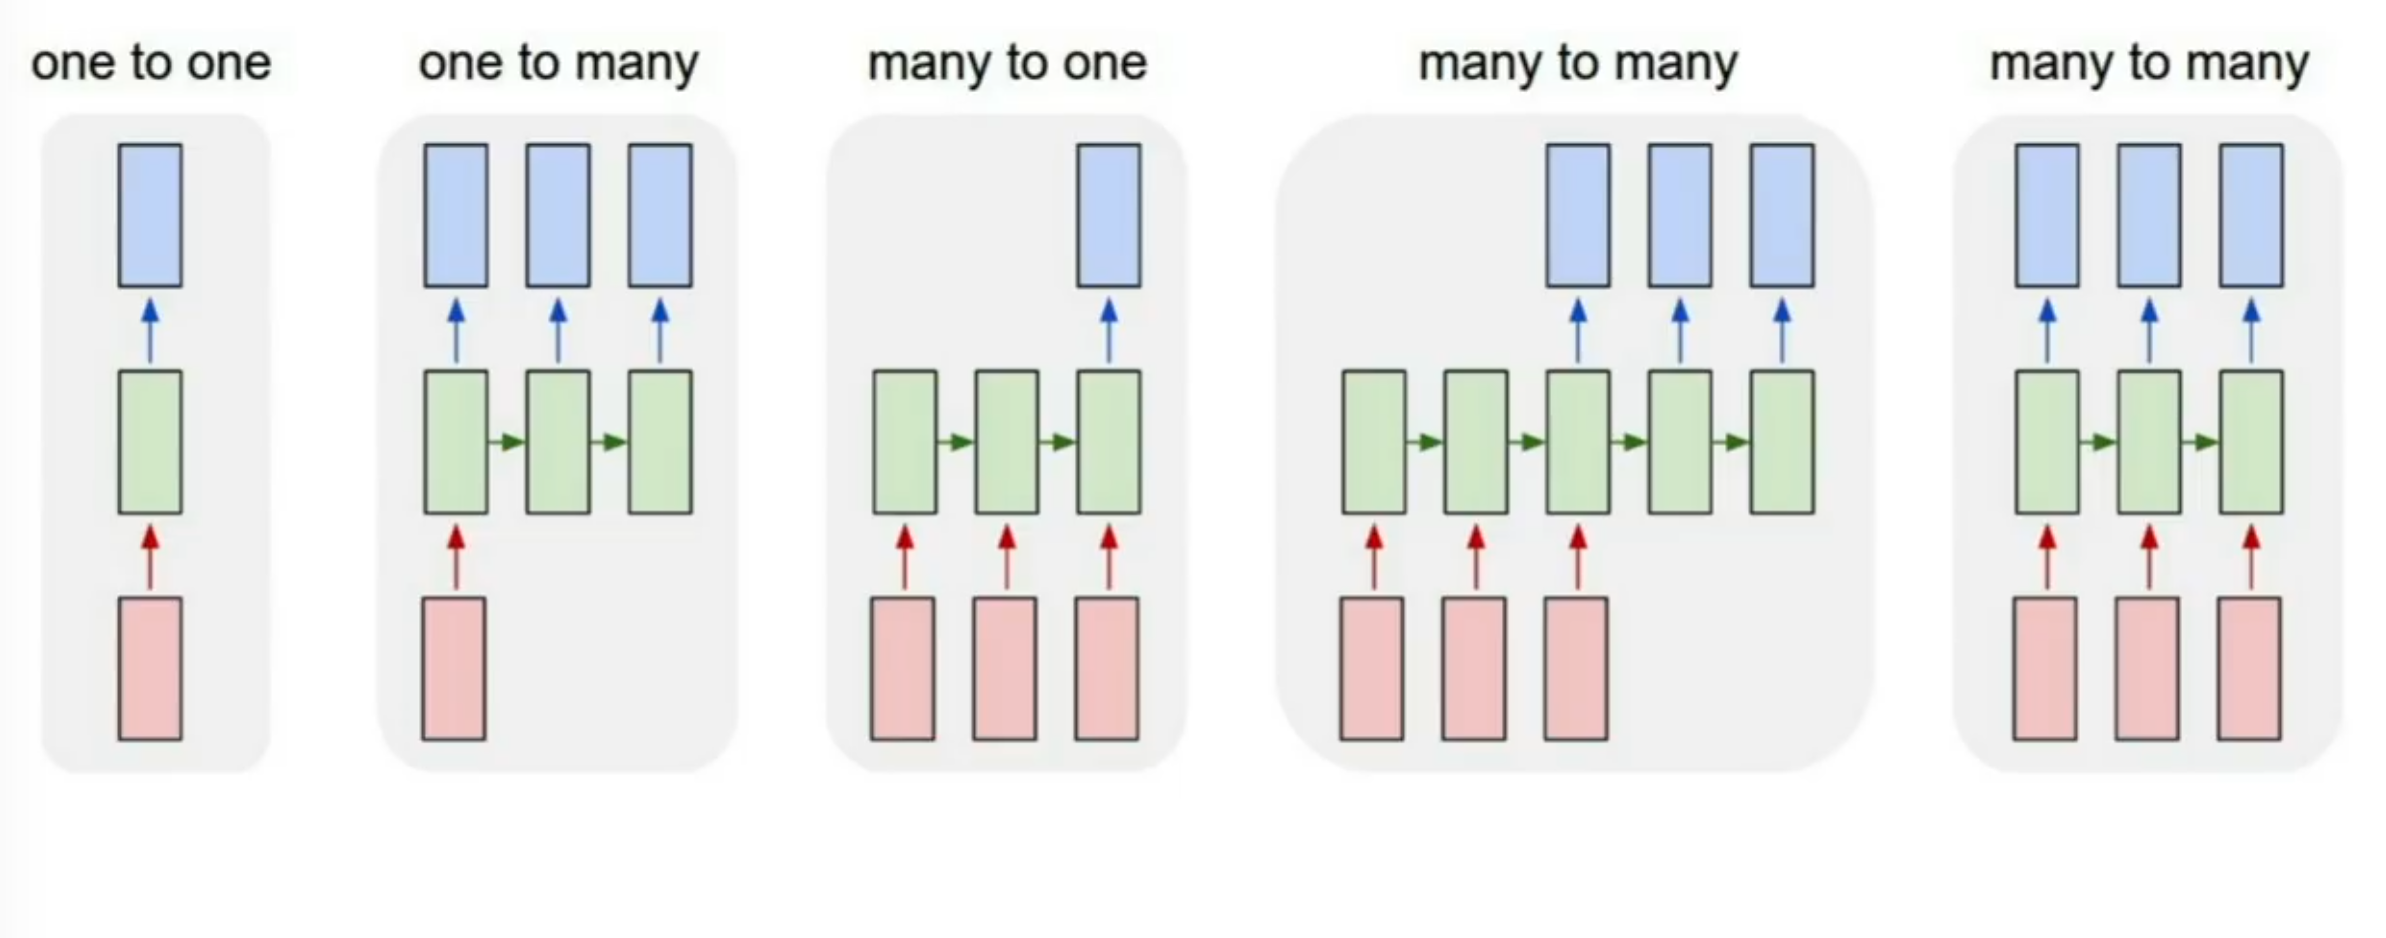
\includegraphics[width=0.15\columnwidth]{fei_fei_li/lecture_10/data_flows.png}

We can have tasks that require a different data flow through the networks. 

The vanilla one to one connection is called  feed-forward network. 

one to many $\rightarrow$ image captioning - for example, image to sequence of texts

many to one $\rightarrow$ variable size input -> for example, labelling text, or labelling video

many to many (1) $\rightarrow$ machine translation, variable length sequences of inputs and outputs

many to many (2) $\rightarrow$ video classification on frame level

\subsubsection{RNN}

% 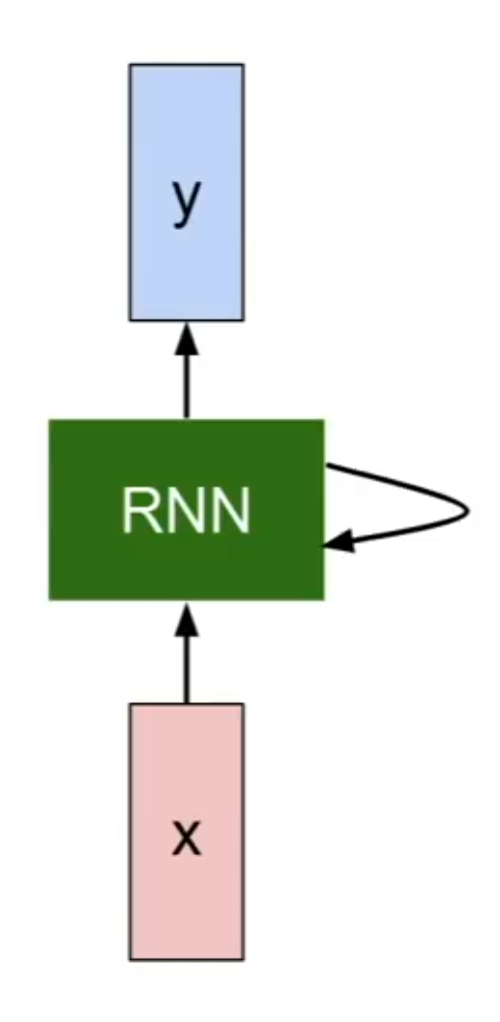
\includegraphics[width=0.5\columnwidth]{fei_fei_li/lecture_10/rnn.png}

$$h_t = f_W(h_{t-1},x_t) $$

$h_t$ new state

$h_{t-1}$ - old state

$x_t$ -  input vector at some time step

$f_W$ some function with params

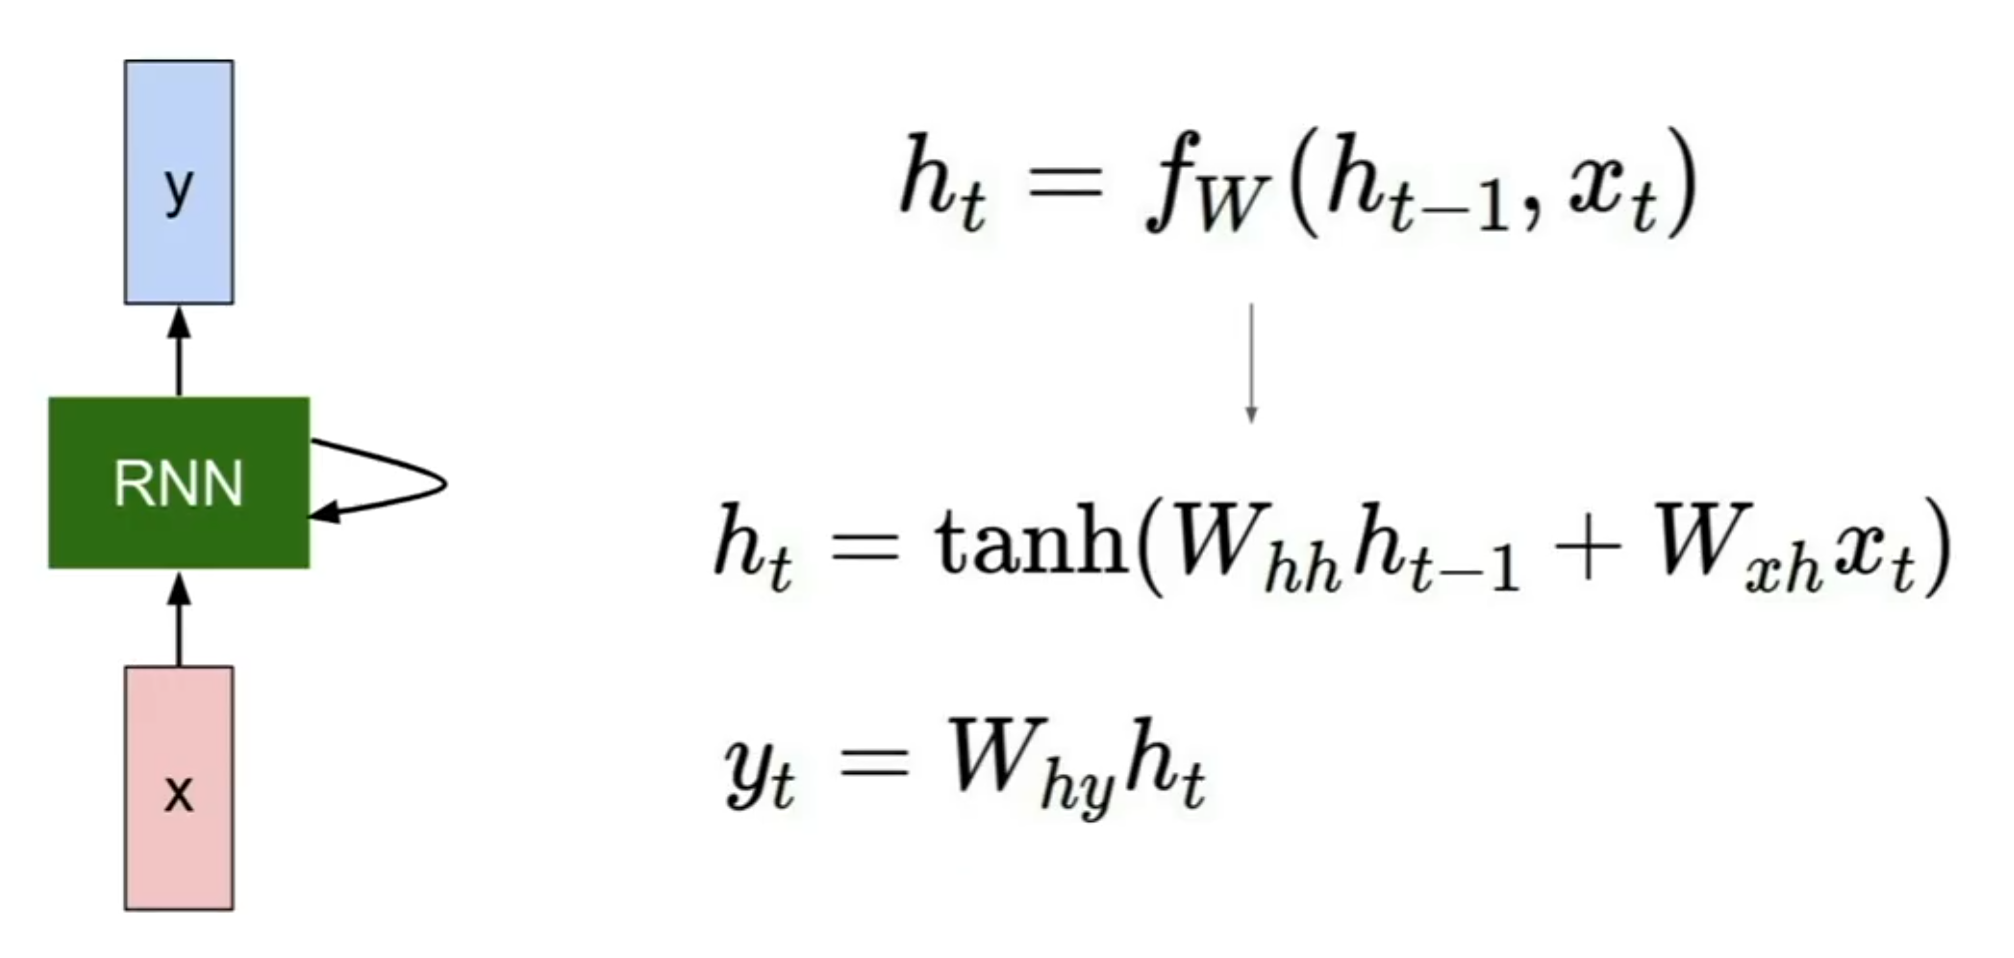
\includegraphics[width=0.5\columnwidth]{fei_fei_li/lecture_10/rnn_formulation.png}

RNN Unrolling: W remains constant throughout the optimization

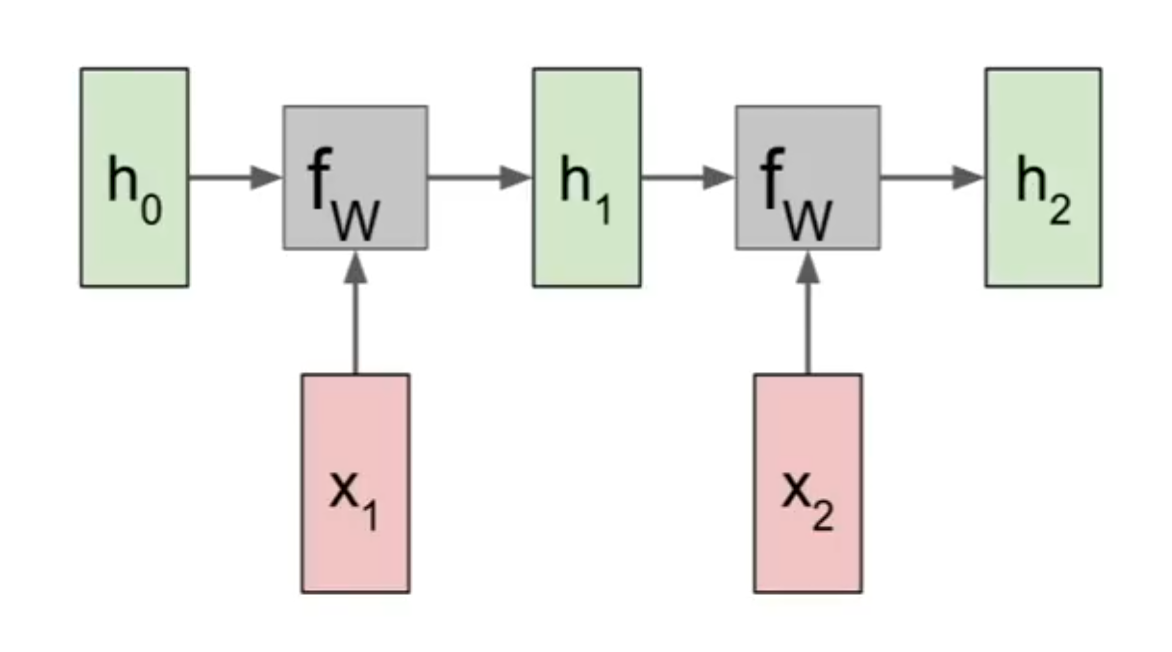
\includegraphics[width=0.5\columnwidth]{fei_fei_li/lecture_10/rnn_unrolling.png}

Many to many - we can get output at every step

Many to one - we will get output based on the final state at the end of the input

One to many - unroll the graph for each cel in the output

Sequence to sequence: encoder and decoder

Encode input sequence in a single vector

Decoder network - one to many - produce output sequence from single input vector

\subsubsection{Example: Character-level Language Model}

Vocabulary: [h,e,l,o]
Training:"hello"

Sampling from the model: seed the model with input

the output layer will have scores with a probability distribution

we can sample from it with softmax and synthesize the next sequence

why sample? 

hard max probability

but sampling let's you get diversity

\subsubsection{Back-propagation through time}

Forward though the entire sequence to compute loss, then backwards though the entire sequence to compute gradient

Very hard to train on long sequences.

Truncated Backpropagation through time - many people use 100 steps. 

Compute a loss over the subsequence of the data

check out min-char-rnn on github for a minimal example of rnn backprop

\paragraph{RNN Attention Models}

RNN can focus its attention on different parts of the image

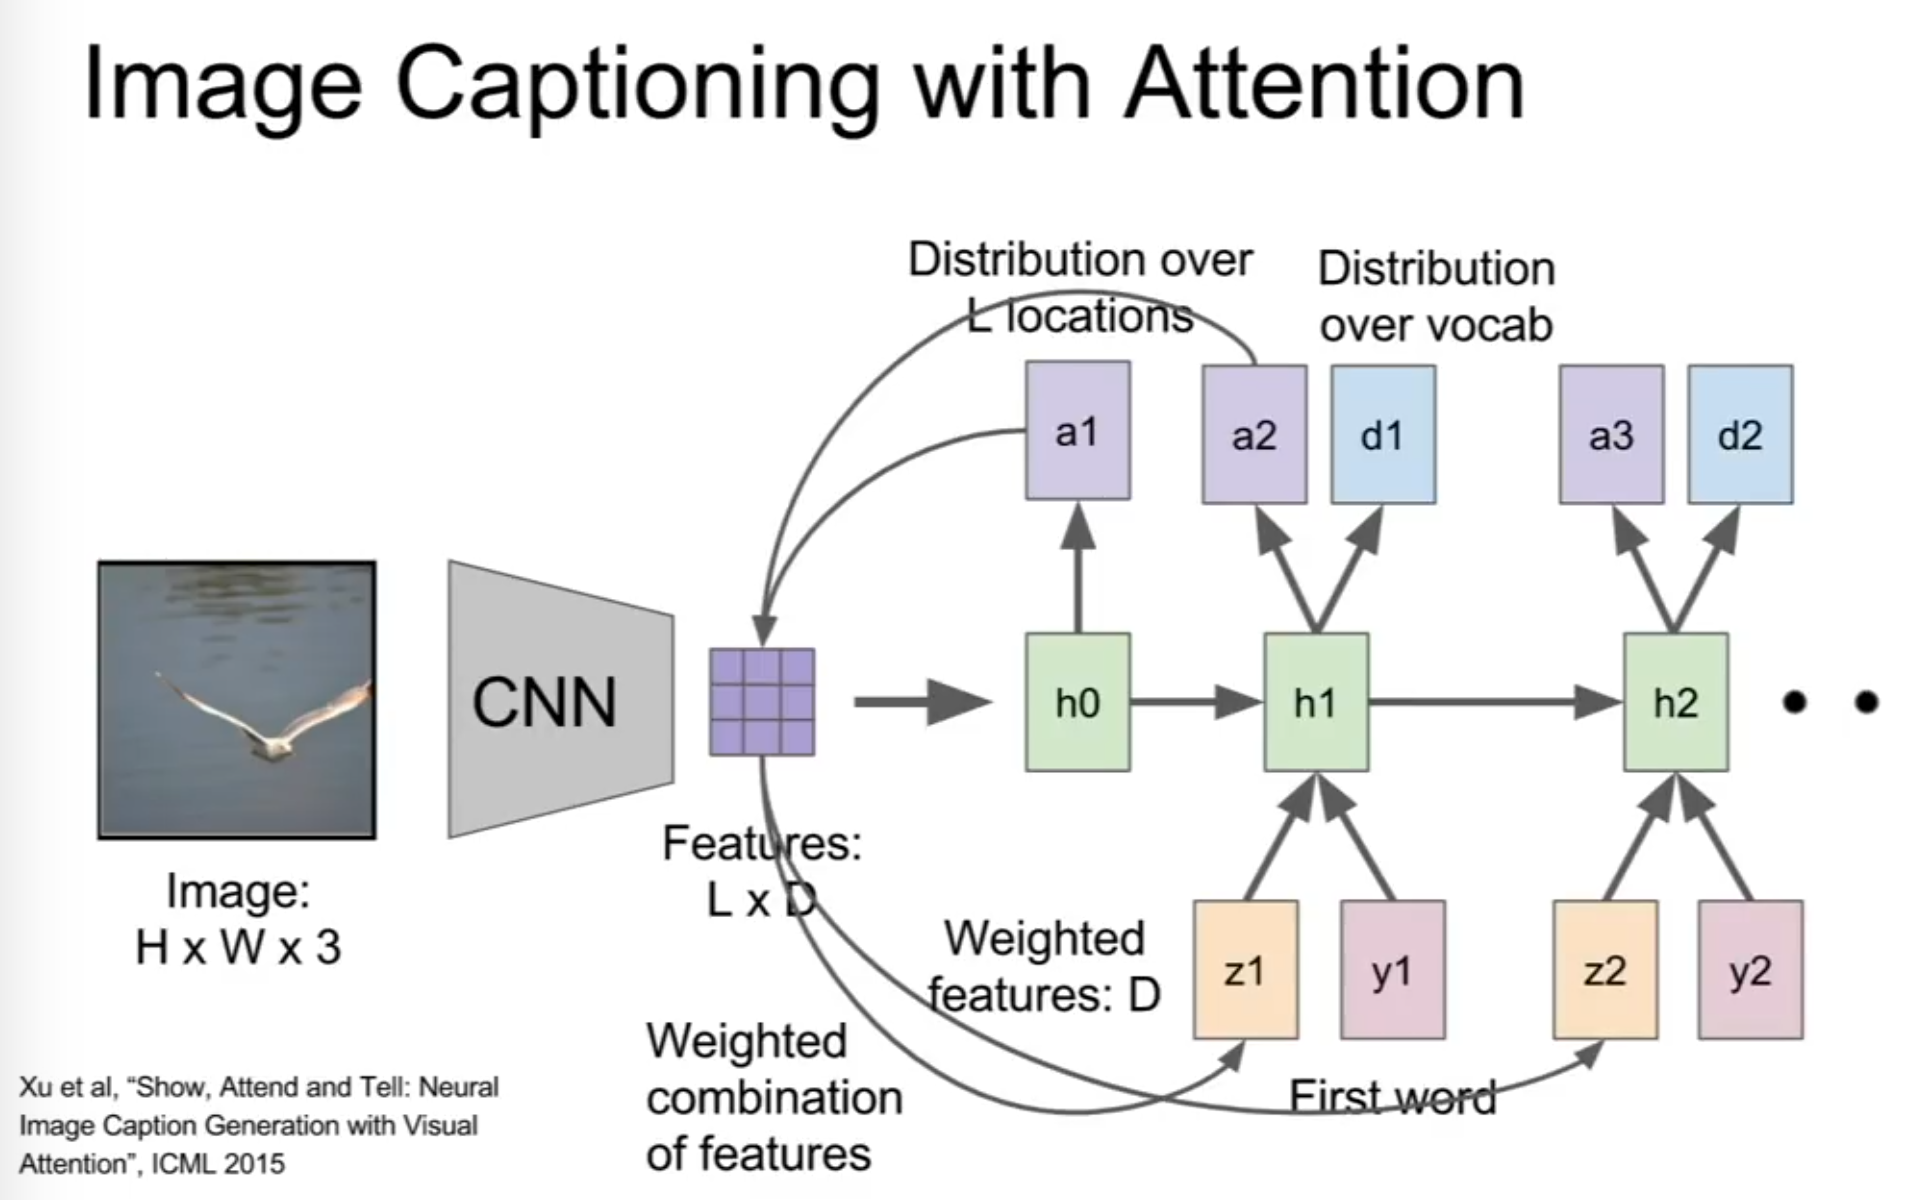
\includegraphics[width=0.5\columnwidth]{fei_fei_li/lecture_10/image_captioning_with_attention.png}

\paragraph{Multi layer RNNs}

max 4 or so

\paragraph{Back propagation of gradient through RNNs}

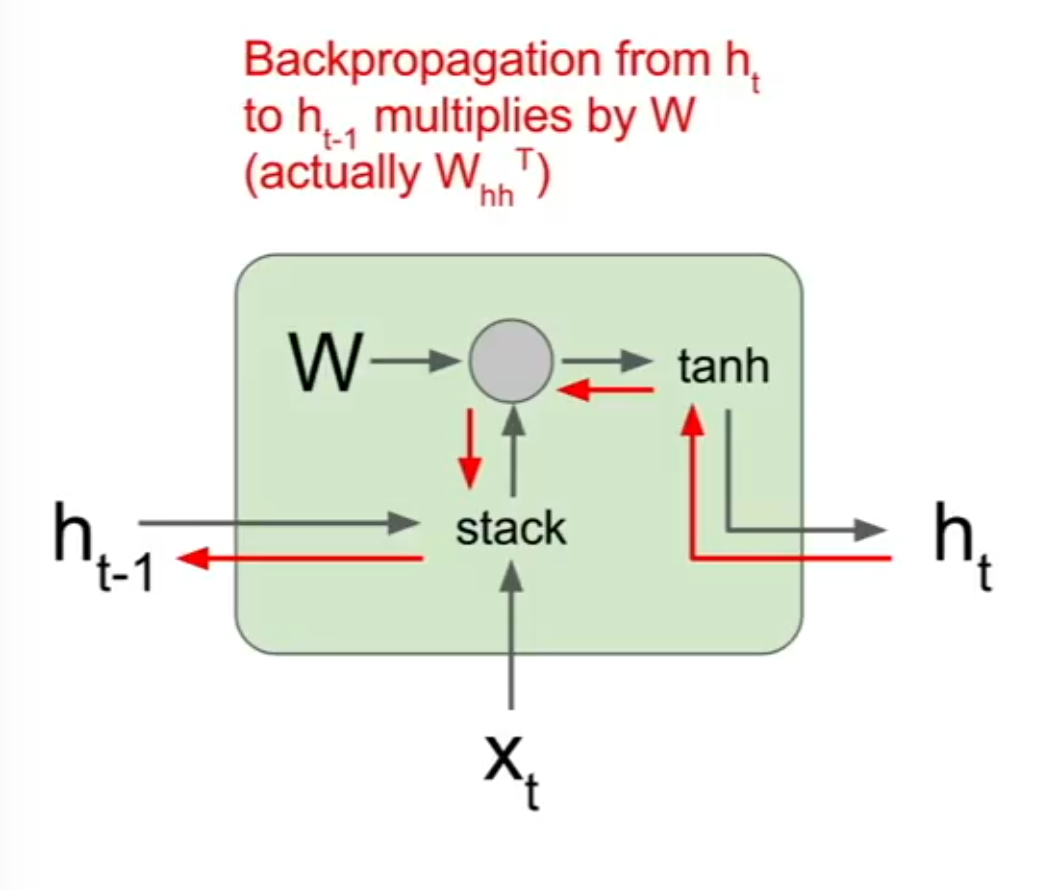
\includegraphics[width=0.5\columnwidth]{fei_fei_li/lecture_10/back_prop_rnn.png}

Gradient through multiple RNN cells: 

Computing the gradient with respect to $h_0$ - we get multiple factors of the $W$ matrix, which can be undesirable. 

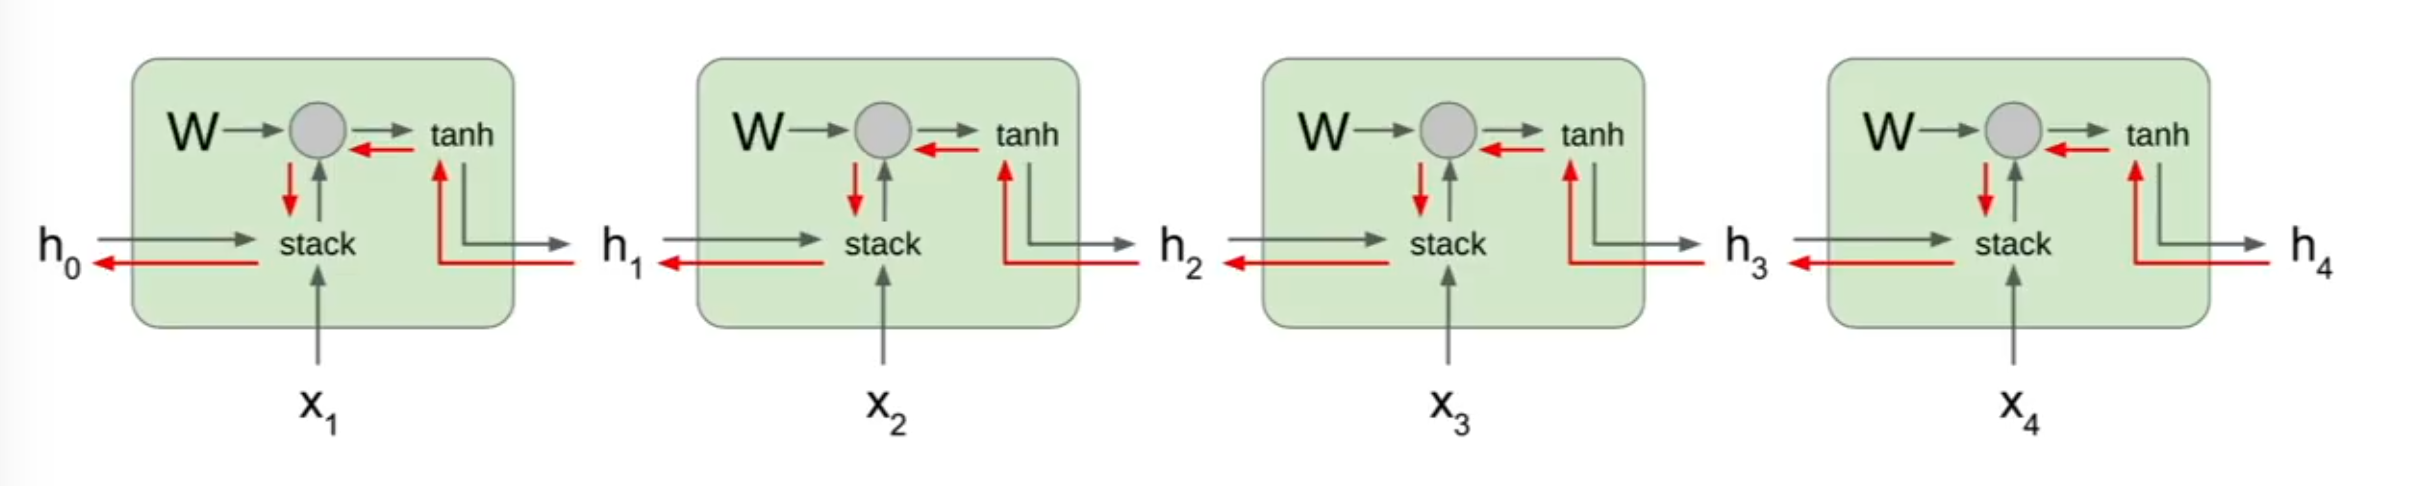
\includegraphics[width=0.5\columnwidth]{fei_fei_li/lecture_10/backprop_multi_layer.png}

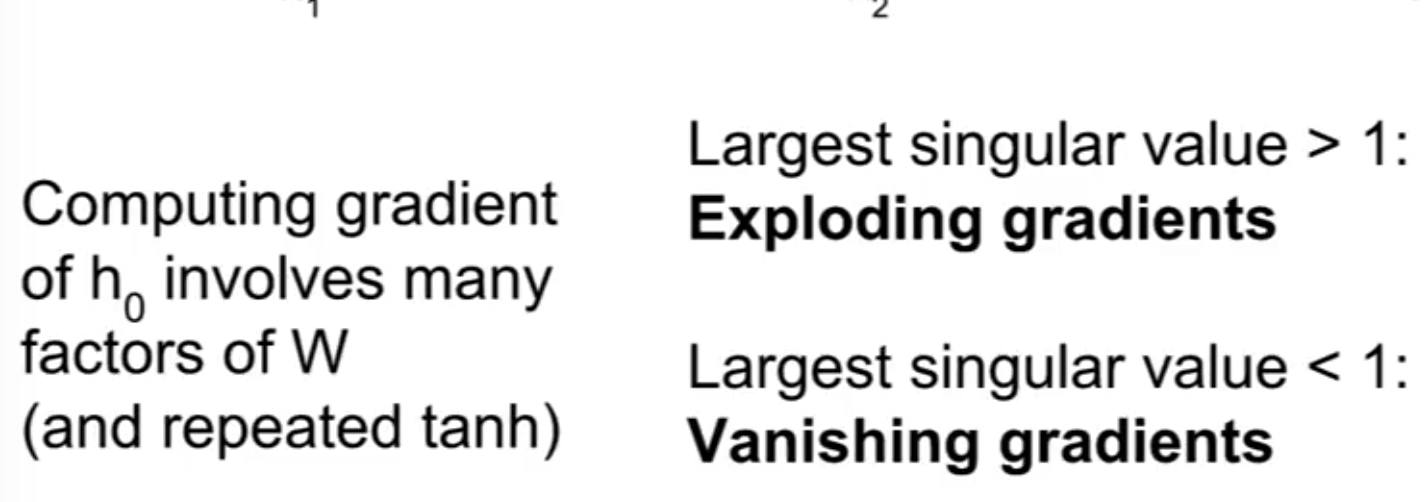
\includegraphics[width=0.5\columnwidth]{"fei_fei_li/lecture_10/gradients.png"}

trick: gradient norm > max threshold, gradient is normalized by its norm

\subsubsection{LSTM}

Long short term memory

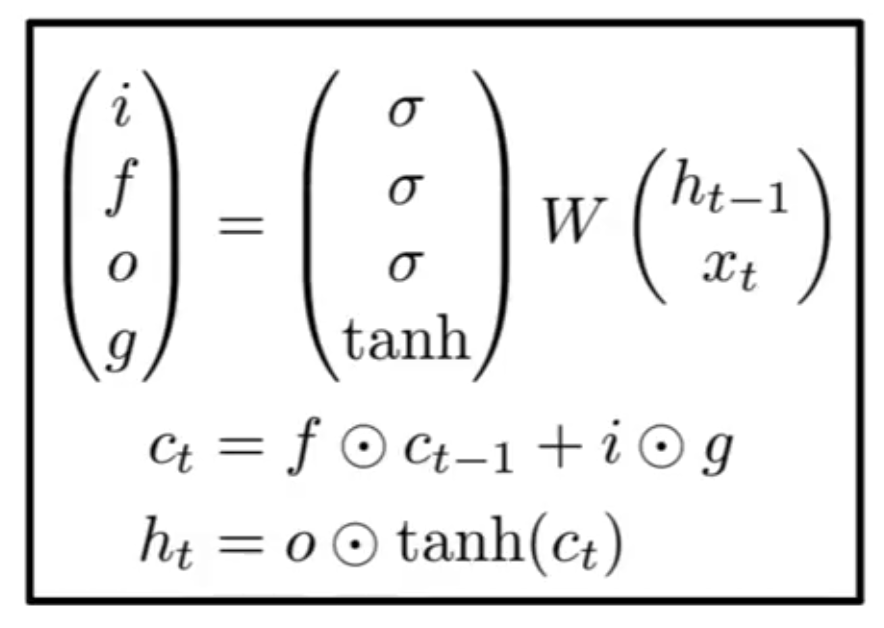
\includegraphics[width=0.5\columnwidth]{fei_fei_li/lecture_10/lstm.png}

better gradient flow properties

$c_t$ cell state - keeps track of the internal state of the cell

we use input to compute the gates i - g

we expose part of the state as the hidden state at the next time step

f - forget gate, wether to erase the cell.

a vector of 0 and 1 which decides for each element wether to use it or not

(element-wise product)
i - input gate, wether to write the cell

similar, but for g gate
g - gate gate - how much to write to cell

o - output gate - how much to reveal cell

at every time step we can remember or forget the internal state, and increment or decrement the state of the cell by 1.

now we squash this into the range of [-1,1] with tanh and the output gate is coming through a sigmoid

the forget gate is coming out of a sigmoid - the forget gate is guarnteed between [0,1]

the output do not flow through tanh

and also there's direct gradient propagation, but i'm not sure about this LSTM stuff

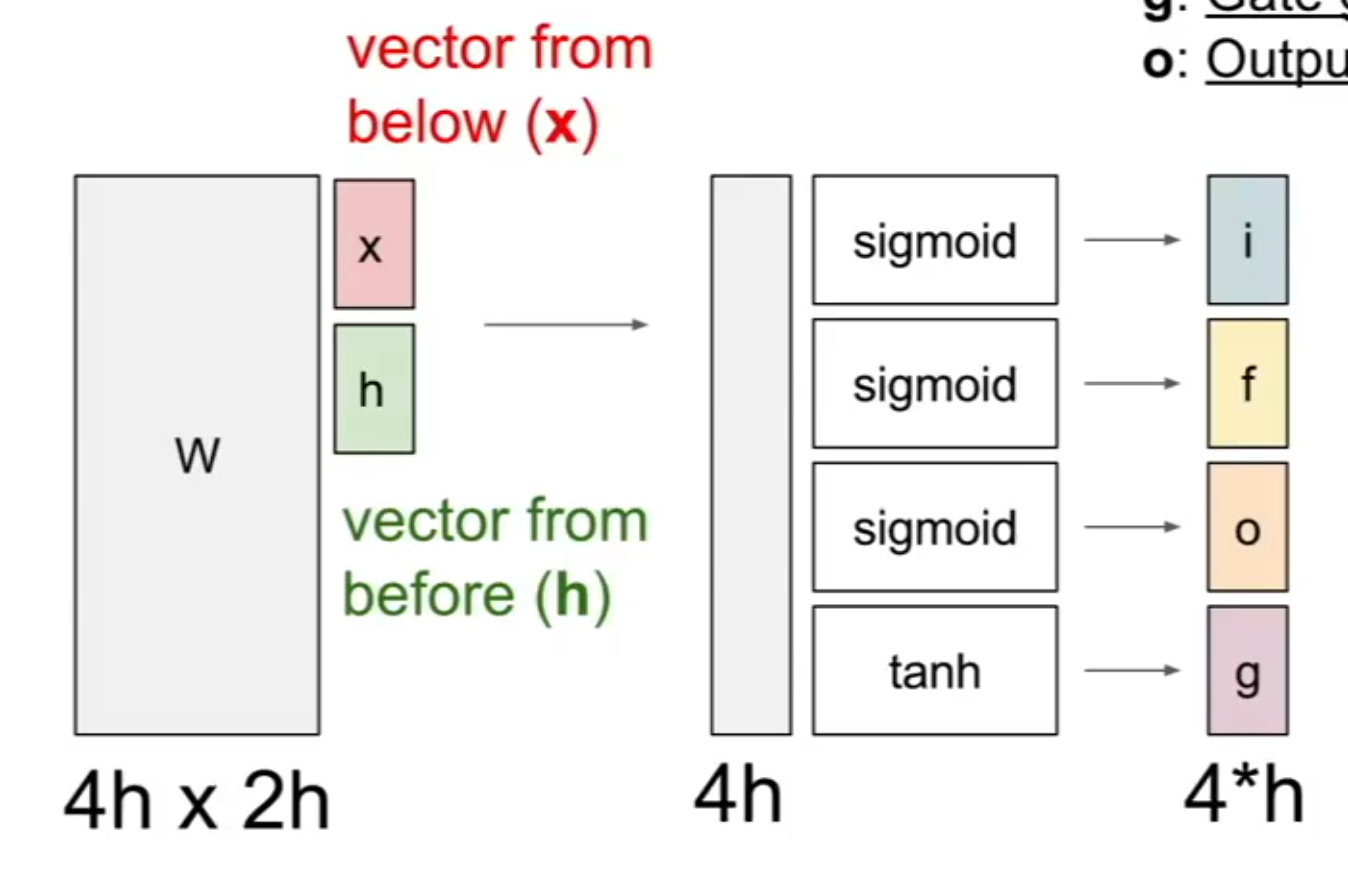
\includegraphics[width=0.5\columnwidth]{fei_fei_li/lecture_10/lstm_arch.png}

$\Rightarrow$ also check out Highway Networks ICML Srivasta

\subsection{Segmentation with CNNs}

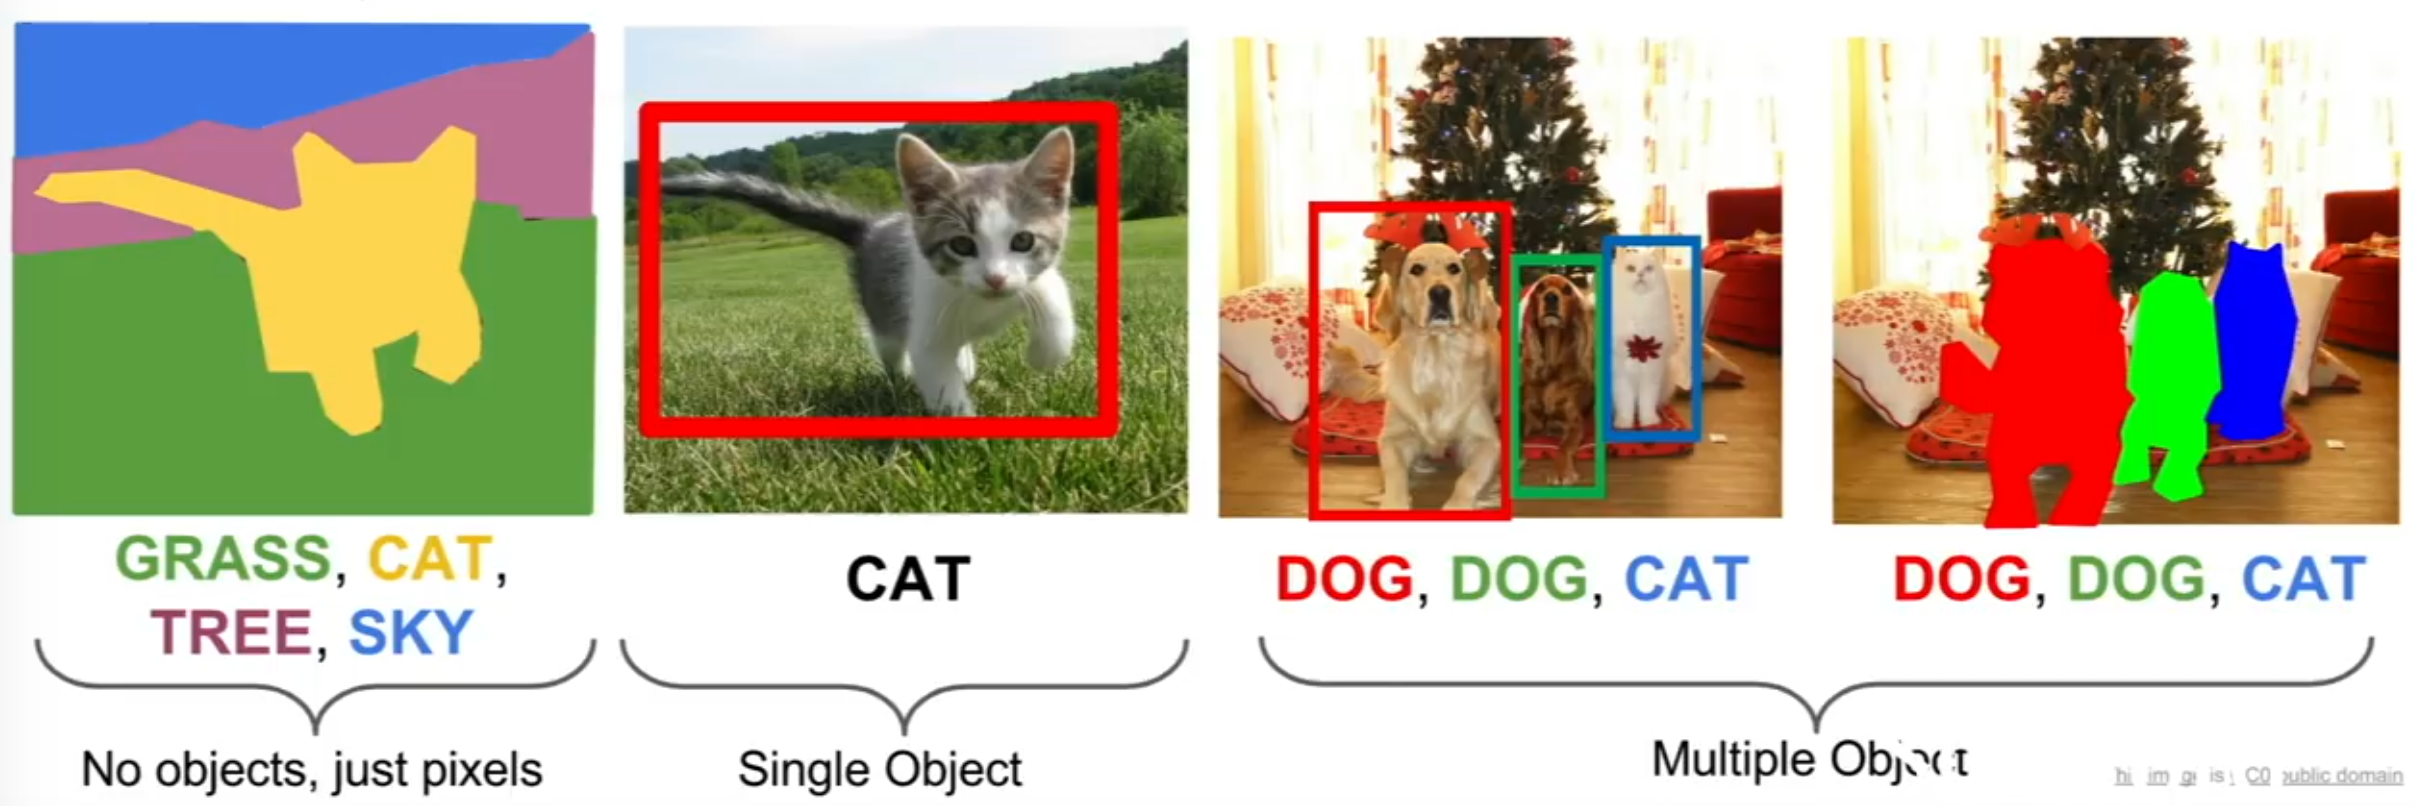
\includegraphics[width=0.5\columnwidth]{fei_fei_li/lecture_11/semantic_segmentation.png}

\subsection{Semantic Segmentation}

Decision for a category for every pixel in that image

Does not distinguish between instances of the object

\subsubsection{Bad Approaches to semantic segmentation}

\paragraph{Approach \#1 - Patch Based}

First idea - but a pretty bad one - patch based classification (sliding window)

extract a patch

classify center pixel with CNN

Computationally expensive and does not share computation for similar patches.

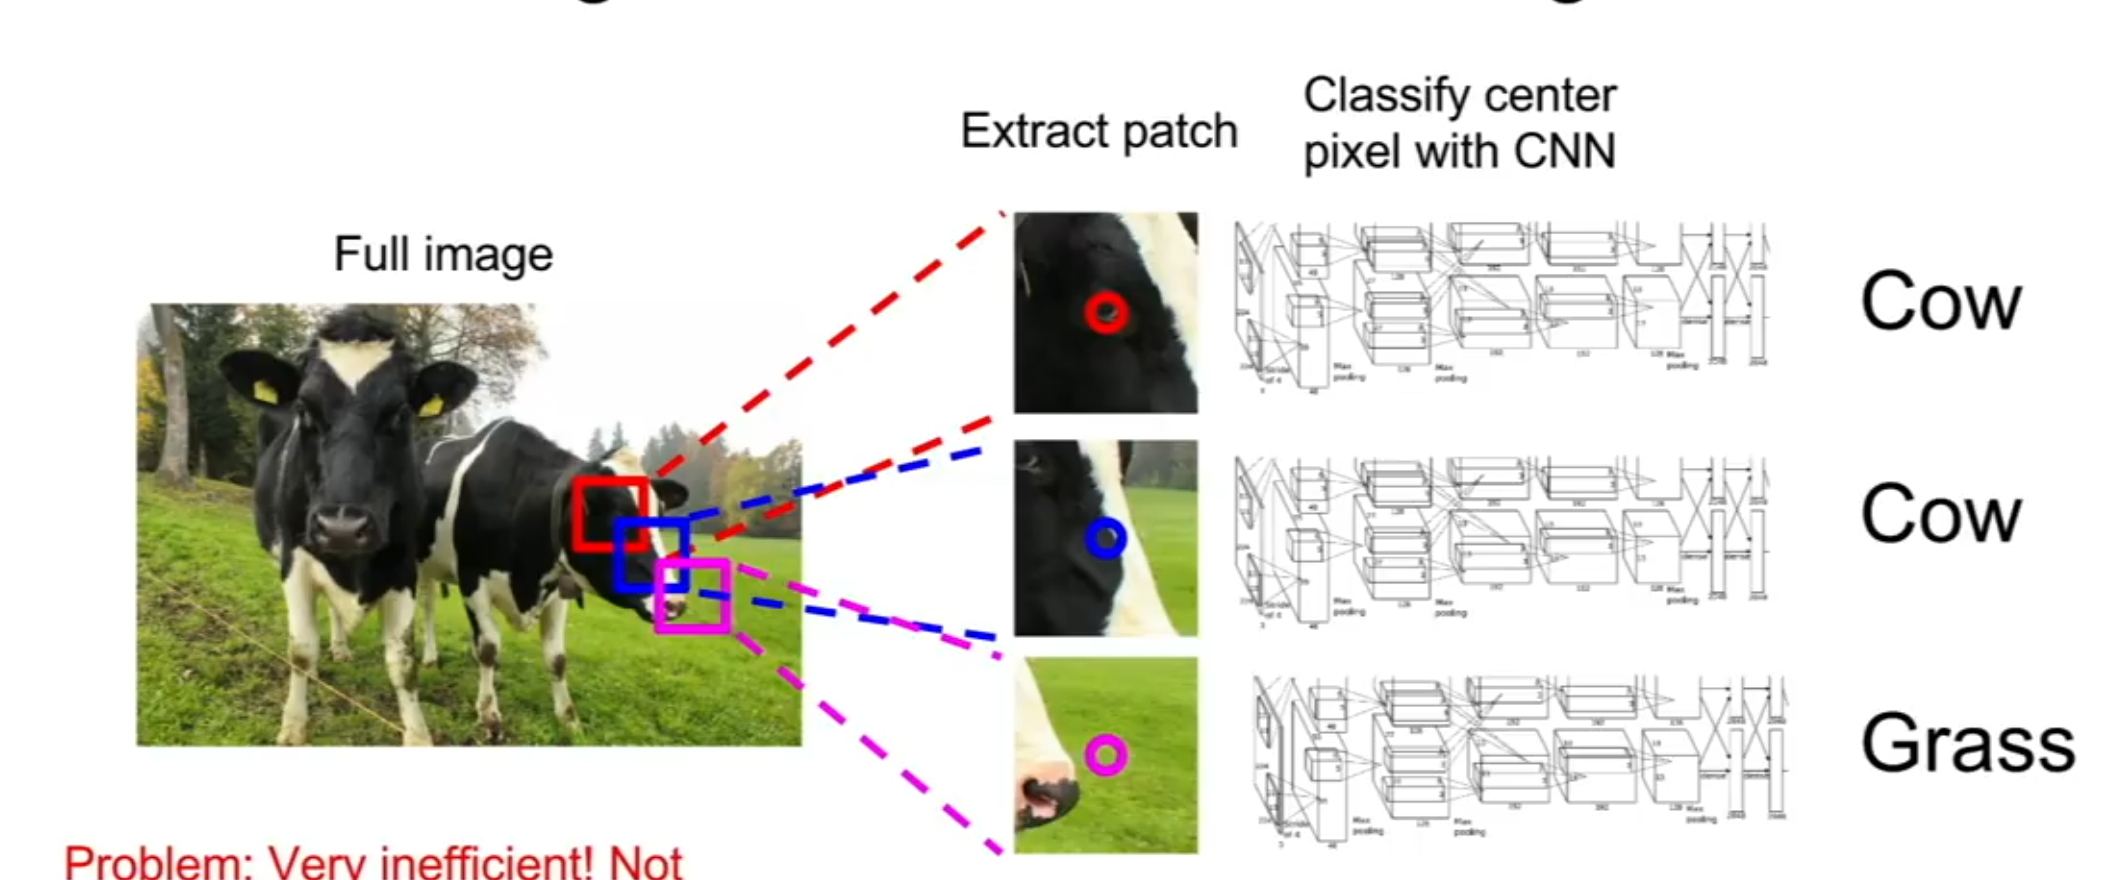
\includegraphics[width=0.5\columnwidth]{fei_fei_li/lecture_11/patch_based.png}

\paragraph{Approach \#2 - Fully convolutional}

Design a network as a bunch of conv layers

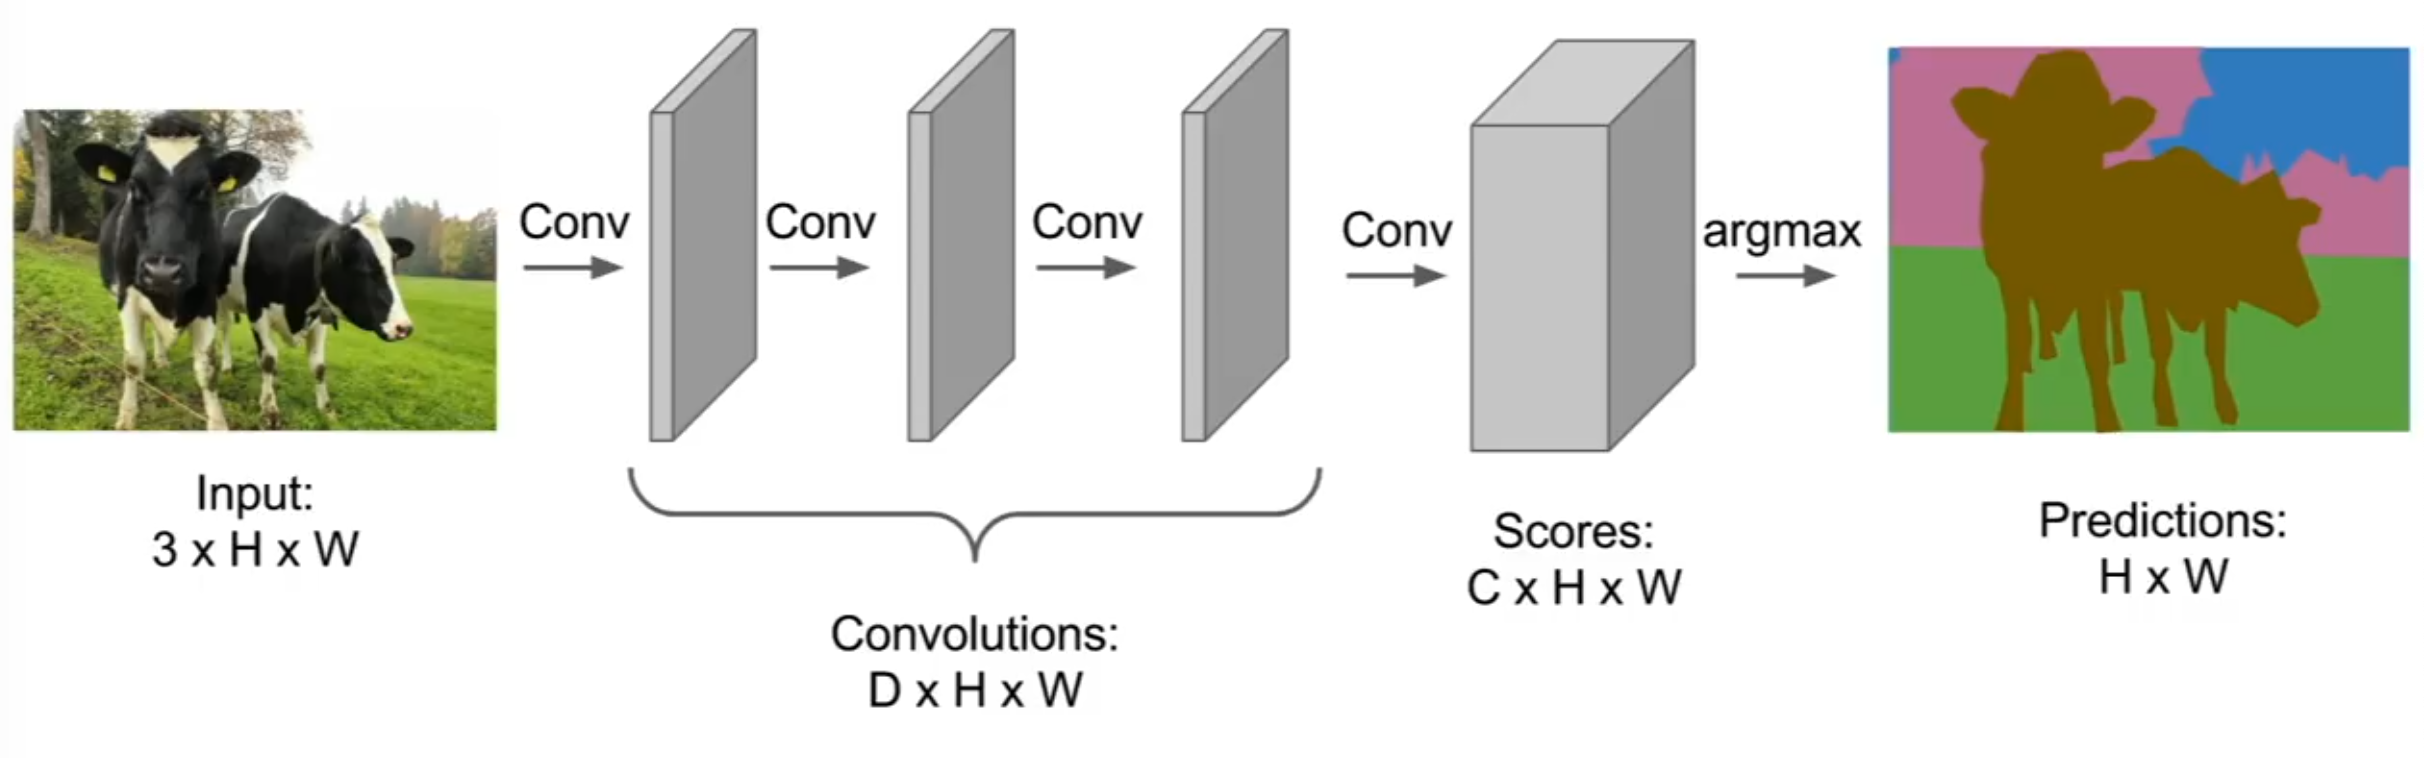
\includegraphics[width=0.5\columnwidth]{fei_fei_li/lecture_11/fully_convolutional.png}

- applying a bunch of conv that all have the same size of the image - very expensive!

\subsubsection{Approach \#3 - Down and upsampling}

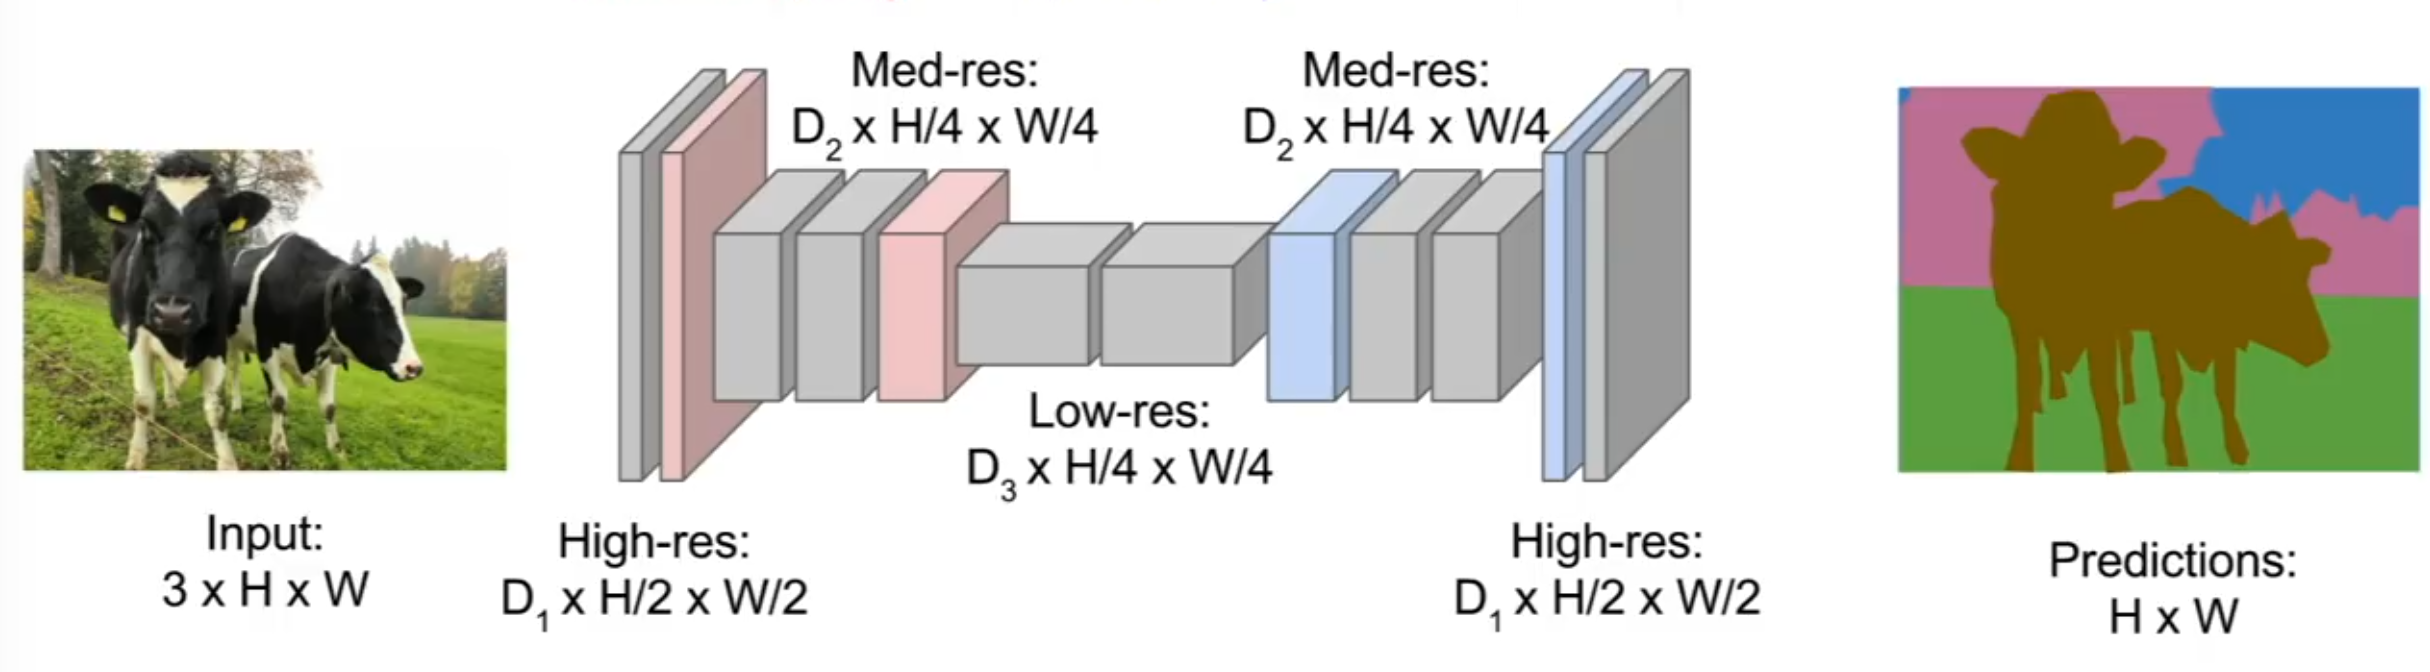
\includegraphics[width=0.5\columnwidth]{fei_fei_li/lecture_11/down_up_sampling.png}

In the second half of the network, the network will typically upsample the data

\paragraph{Unpooling}

Nearest Neighbor:

\includegraphics[width=0.5\columnwidth]{fei_fei_li/lecture_11/nn_uppooling.png}

Bed of nails:

\includegraphics[width=0.5\columnwidth]{fei_fei_li/lecture_11/bed_of_nails.png}

Max Unpooling:

\includegraphics[width=0.5\columnwidth]{fei_fei_li/lecture_11/max_unpooling.png}

\subsubsection{Learnable Upsampling - Transpose Convolution }

\includegraphics[width=0.5\columnwidth]{fei_fei_li/lecture_11/learnable_conv.png}

When the receptive fields in the output overlap, we sum

Sometimes called: 

- deconvolution

- upconvolution

- fractionally strided convolution 
- stride 1/2 convolution - if the stride is the relation between the input and output

- backward strided convolution

Convolution can be framed as matrix multiplication: $\vec x \star \vec a = X\vec a$

If we do a transpose to the $X$ matrix we get the "deconvolution" operation

\includegraphics[width=0.5\columnwidth]{fei_fei_li/lecture_11/trans_conv_math.png}

\subsubsection{Classification + Localization}

i.e. bounding boxes

assumption: there is exactly one object in the image

can reuse previously familiar arch with one change: now there's a fully connected layer which also returns box coordinates

\includegraphics[width=0.5\columnwidth]{fei_fei_li/lecture_11/class_loc.png}

There are two loss functions:

softmax loss to create labels

L2 loss for the correct boss (simplest)

The assumption is that the images are labelled with these

The idea is that we have regression loss (what's that?)

multi task loss - have an additional hyperparamter that is used to scale both loss types, and take the gradient in respect to the weighted sum

the weighted hyperparamter changes the value of the loss function, which makes it harder to compute the gradient - cannot compare diff values for the hyperparamter directly as it directly affects the value of the loss

to deal with this: use some other metric of performance

better performance to train the network jointly

another possibility: freeze the network, train other parameters, and then fine tune the entire network

\paragraph{Human Pose Estimation}

Represent pose as a set of 14 joint positions

\subsubsection{Object Detection}

Different from localization - might have many number of outputs

\paragraph{Sliding window}

Different crops from the image - feed it through a classification network

We also add a category of background if it cannot find

Problem: how do you choose the crops? location, size, aspect ratio, etc.

\paragraph{Region Proposal Network}

Will generate boxes where objects may be present.

Relative fast to run - Selective Search

High recall, and also many regions without objects.

\subsubsection{R-CNN}

Put together all of the pipeline: 

Extract ROIs form proposal method

Warp ROIs to the fixed size for the downstream network

Run through CNN

Use SVM to compute grades (svm loss - hinge loss)

In addition, predict correction to the bounding box

Multi class loss, train the whole thing

Main problem: super slow on training and inference

\paragraph{Fast RCNN}

forward the whole image through convnet

create feature map of the image

roi pooling layer

fully connected layer

bounding box regressor

\includegraphics[width=0.5\columnwidth]{fei_fei_li/lecture_11/fast-rcnn.png}

During training add a multi class loss to do regression and do back prop:

\includegraphics[width=0.5\columnwidth]{fei_fei_li/lecture_11/fast_rcnn_2.png}

fast RCNN runtime is still dominated by the procedure to find ROIs.

\subsubsection{Faster RCNN}

Make the CNN do proposal 

Have to optimize for four! different tasks/ goals which might be tricky

Training ROI is tricky because there's no ground truth data - to do this, any overlap between ROIs and ground truth object is marked as positive and cases of no intersection are given a negative rating

Classification task - binary decision for each region

Removed the overhead from computing region proposals.

Once you're learning ROIs, you can bias the model to your data.

\subsubsection{Detection without Proposal}

The idea for both of this methods is to do object detection as a regression problem, and perform all of the tasks at once.

\includegraphics[width=0.5\columnwidth]{fei_fei_li/lecture_11/YOLO_SSD.png}

\paragraph{YOLO}

YOLO - you only look once

Feed forward single pass object detection.


\paragraph{SSD - Single Shot Detection}

\subsubsection{Instance Segmentation}

Predict the location and identities of the objects in the image

Rather than predict a bounding box, predict a segmentation mask for each of these objects.

\paragraph{Mask R-CNN }

Similar to Faster RCNN

Instance segmentation was trained on the Microsoft Coco dataset

\subsection{Visualization and Understanding}

\subsubsection{First Layer}

We can visualize each one of the filters directly:

We're visualizing the RGB layers from first layers of the filters. 

Observing  strong response to oriented edges in opposing colors

(this is from the pytorch model zoo)

\includegraphics[width=0.5\columnwidth]{fei_fei_li/lecture_12/first_layer_vis.png}

Visualizing higher level layers weights are less obvious - 16 channel input

16x20x7x7 filters?

\subsubsection{Last fully connected layers:}

\subsubsection{The last layer visualization}

4096d feature vector for an image

Nearest neighbors in feature space:  run all images through the network and collect the feature vectors

Can potentially be very different from in appearance, but similar in semantic content

There is nothing in the loss function that encourages these features end up close together.

\paragraph{Dimensionality Reduction}

Visualize the space of TC7 by reducing the dimensionality of the vectors from 4096 to 2 dimensions?

PCA

t-SNE

\paragraph{Maximally Activating Patches}

Keep track of what patches maximally activate neurons from a dataset and visualize them - gives an idea of what kind of features the neuron might be looking for.

\paragraph{Occlusion Experiments}

Check which parts of the image cause the largest change in the classification / probability / scores

\paragraph{Saliency Maps}

Visualize which pixels matter most for classification

Compute the gradient of (unnormalized) **class score** with respect to image pixels, take abs value and max over rgb channels.

This tells us how much the class score changes with the respect of each pixel

GrabCut + Saliency maps

\paragraph{Guided Back Propagation}

compute the gradient of neuron value with respect to image pixels

now in addition to the patches, we can see exactly which part of patch activates the neuron

\includegraphics[width=0.5\columnwidth]{fei_fei_li/lecture_12/patches.png}

\paragraph{Gradient Ascent}

Synthesize images that maximize the activation in the network.

Start with a neutral image, compute gradient with respect to the neuron you want to maximize, and update the image in that direction

For regularization: just regularize the $L_2$ norm of the image

Some people do stuff like 

- clipping pixel values

- gaussian blur image

This can be interpreted as projection of this max image onto a nicer image space

$\Rightarrow$ Visualizing this features and neurons would be a good exercises for me

Visualizing the higher level features shows that some of the class labels are multi modal

\subsubsection{Adversarial Examples}

Idea: 

1. start from an arbitrary image
2. pick arbitrary class
3. modify the image to maximize the class
4. repeat until network is fooled

\subsubsection{Feature Inversion}

Total variation - encourages absolute pixel differences between neighboring pixels - encourages spatial smoothness

\subsubsection{Natural Feature Synthesis}

~50 minutes into the lecture, i don't care about this

\paragraph{Texture Generation}

Nearest neighbor - simple approach that works pretty well for simple textures

March through the generated image and look at neighborhood around current pixel

But more complex texture do not work so well

Similar to gradient ascent in CNN

Gram Matrix -  

\subsubsection{Style Transfer}

\includegraphics[width=0.5\columnwidth]{fei_fei_li/lecture_12/text_synthesis.png}

The $C\times C$ matrix can be used as a feature descriptor, to describe which features tend to activate together the most.

The matrix throws away all spatial information because it averages all feature pairs in the image. 

Efficient to compute - 

$$ C \times H \times W \Rightarrow C \times HW \\$$ 

Using true covariance matrix also works but it is more expensive to compute

The gram matrix can be used to generate images with the same matrix:

\includegraphics[width=0.5\columnwidth]{fei_fei_li/lecture_12/texture_synthesis.png}

Using higher layers of features from the CNN results in larger features being reconstructed or transferred into the test image

\subsubsection{Style Transfer}

Feature matching + texture synthesis

Input: Content Image + Style Image

Minimize the feature reconstruction loss of content image and minimize texture loss on for texture image

\includegraphics[width=0.5\columnwidth]{fei_fei_li/lecture_12/style_transfer.png}

(might take a few hundred iterations to converge)

Can play with parameters - tradeoff between content and style

Resizing the style image gives control on the features which are going to be transferred

Problem: slow - many forward and backward passes.

Solution: train CNN to do the style transfer

Train (a few hours) - then single forward pass

Runs in real time

Fast style transfer - replaced batch normalization with instance normalization 

Google addressed this by training one network to do style transfer to many different styles

\section{Generative Models}

\subsection{Unsupervised Learning}

The strategy is: 

Data -> encoder -> features -> decoder -> reconstruction

The loss is trying to create a good reconstruction of the input data

Can be $L_2$ loss

Examples: 

Data: just data

Goal: learn the underlying hidden structure of the data

Examples: clustering, dim reduction, feature learning, density estimation

\paragraph{Density Estimation}

\includegraphics[width=0.5\columnwidth]{fei_fei_li/lecture_13/density.png}

In the unsupervised version, the data is cheap.



\subsection{Generative Models}

A class of models, where, given training data, the goal is to generate more examples from the same distribution.

Address density estimation 

- Explicit density estimation
- Implicit density estimation

Why?

- Realistic samples from artwork 

- Super-resolution

- Generative models of time-series data for simulation and planning

  - Good for reinforcement learning

- Learning latent variable representation

  \includegraphics[width=0.5\columnwidth]{fei_fei_li/lecture_13/taxonomy.png}

(for Ian Goodfellow tutorial on generative models)

\subsubsection{Pixel RNN + PixelCNN}

Fully visible belief networks:

Explicit density model

$p(x) = \Pi_{i=1}^n p(x_1 | x_1,\dots, x_{i-1})$ 

likelihood of the image $x$, the likelihood of each pixel given all previous pixel values

this is a complex transformation, we use NN 

Q: how to order the pixels?

\paragraph{PixelRNN}

Generate image pixels starting with one corner

Depending on previous pixels using a RNN with LSTM

Sequential generation - slow

\paragraph{PixelCNN}

Still generates an image from a corner

Use CNN to model the dependency over a context region

output: softmax loss at each pixel

$\Rightarrow$ i don't get it



\subsubsection{Autoencoders}

Input $(X)$ -> Encoder -> (Latent) Features (Z)

$dim(Z) < dim(X)$ - the features should capture the \emph{important} variation in the data

Encoders: linear, non linear, ReLU, 

Train the model as features that be used to reconstruct the original data

Decoder: usually same types of networks as the encoder.

\includegraphics[width=0.5\columnwidth]{fei_fei_li/lecture_13/encoder_decoder.png}

After this step, we don't need to decoder anymore - we can use this to initialize a supervised model:

\includegraphics[width=0.5\columnwidth]{fei_fei_li/lecture_13/supervised_encoder.png}

For example, this is used in cases where there is not a lot of data.

Autoencoders can reconstruct data and learn new features to initialize a supervised model. 

The features capture the variation in the training data. Now how can we use them to generate new data?

\subsubsection{Variational Autoencoders}

Probabilistic spin on autoencoders - will let us sample from the model to generate data.

Assuming training data $\{x^{i}\}_{i=1}^N $ is generated  from underlying, unobservred latent representation $z$ 

Generation process: sample from a prior over $z : p_{\theta^\star}(z)$  usually a Gaussian 

Now sample from true conditional: $p_{\theta^\star}(x|z^i)$ \includegraphics[width=0.5\columnwidth]{fei_fei_li/lecture_13/decoder_training.png}

Want to estimate the true parameters $\theta^\star$ so we can generate new data.

Gaussian assumption is reasonable for latent attributes such as pose, expression etc.

The conditional representation $p(x|z)$ is much more complex and it is represented through a network (decoder neural network)

How to train this model?

From Fully Visible Belief Networks: learn  model parameters to maximize the likelihood of training data:

$p_\theta(x) = \int p_\theta 	(z) p_\theta(x|z)dz$ 

This integral is intractable - it is impossible to integrate over all z

Posterior density is also intractable: $$p_\theta(z|x)=p_\theta(z)/p_\theta(x) $$

The solution is to define another encoder network $q_\theta(z|x)$ that approximates $p_\theta(z|x)$. This allow us to derive a lower bound on the data likelihood which is tractable. 

The encoder network will give out the mean and covariance of $z|x$:

\includegraphics[width=0.5\columnwidth]{fei_fei_li/lecture_13/encoder_theta.png}

and similarly we have a probabilistic decoder network:

\includegraphics[width=0.5\columnwidth]{fei_fei_li/lecture_13/prob_decoder.png}

Both of these network produce distributions, we can sample from them $x|z$ and $z|x$ .

These network types are also known as recognition and inference and generation networks

\subsubsection{Recap:}

- PixelCNNs define tractable density function, optimize the likelihood of training data

- VAE define intractable density function with latent $z$, - but cannot be optimized directly, instead derive and optimize lower bound on the prob. dist.
- GANs - give up on explicitly modeling density, just want to sample

\subsubsection{Generative Adversarial Networks}

Want to sample from a complex, high dimensional training distribution.

To actually do this, we sample from a simple distribution (random noise) and use a network that learned a transformation from this to the training distribution.

\includegraphics[width=0.5\columnwidth]{fei_fei_li/lecture_13/gans_1.png}



To learn this transformation network is to look at this as two player game:

Generator Network: try to fool the discriminator by generating real looking images.

Discriminator network: try to distinguish between real and fake images.

\includegraphics[width=0.5\columnwidth]{fei_fei_li/lecture_13/gan_pipeline.png}

Both networks are jointly trained as a minimax game:

$$ \min_{\theta_g} \max_{\theta_d} \left[ \mathbb{E}_{x\sim p_{data}}\log D_{\theta_d}(x)+\mathbb{E}_{z\sim p(z)}\log(1-D_{\theta_d}(G_{\theta_g}(z))) \right]$$

The discriminator outputs likelihood in  $(0,1)$ of real images

The first term is the disc output for real data $x$ drawn from $p_{data}$

The second D term is the discriminator output for generated fake data.

The discriminator $\theta_D$ wants to maximize this objective - $D(x)$ is close to 1 $D(G(z))$ is close to 0 (fake data)

The generator $\theta_z$  wants to minimize the objective s.t. $D(G(z))$ is as close to 1

The optimization to do this goes as follows: 

1. Gradient ascent on the discriminator

   $$ \max_{\theta_d} \left[ \mathbb{E}_{x\sim p_{data}}\log D_{\theta_d}(x)+\mathbb{E}_{z\sim p(z)}\log(1-D_{\theta_d}(G_{\theta_g}(z))) \right]$$

2. Gradient descent on the generator:

   $\min_{\theta_g} \left[ \mathbb{E}_{z\sim p(z)}\log(1-D_{\theta_d}(G_{\theta_g}(z))) \right]$

In practice this does not work very well:

\includegraphics[width=0.5\columnwidth]{fei_fei_li/lecture_13/gan_loss.png}

The gradient is weak when the generator has not learned how to generate good samples yet. So instead we maximize the likelihood that the discriminator is wrong using a different objective:

$\max_{\theta_g} \mathbb{E}_{z\sim p(z)}\log(D_{\theta_d}(G_{\theta_g}(z)))  $

\includegraphics[width=0.5\columnwidth]{fei_fei_li/lecture_13/gan_fixed_loss.png}

Jointly training these two networks is challenging, unstable, etc.

Choosing objective with better loss landscapes helps training.

\includegraphics[width=0.5\columnwidth]{fei_fei_li/lecture_13/full_opt_pipeline.png}

The lecture also shows how the vectors of the params these networks generate are interpretable, for examples mean smiling women - mean neutral women + mean neutral man -> smiling man

\includegraphics[width=0.5\columnwidth]{fei_fei_li/lecture_13/interpetable.png}

Radford et al. ICLR 2016

\includegraphics[width=0.5\columnwidth]{fei_fei_li/lecture_13/year_of_gan.png}



https://github.com/soumith/ganhacks

GAN Summary:

pro: state of the art samples

cons: tricky to train, can't solve inference

\section{Reinforcement Learning }

\subsection{Markov Decision Process}

Markov property: current state completely characterized the state of the world

Define by: $(\mathcal{S,A,R},\mathbb{P},\gamma)$

$\mathcal{S}$ set of possible states

$\mathcal{A}$ set of possible actions

$\mathcal{R}$ set of possible rewards given state, action pair 

$\mathbb{P}$ transition probability

$\gamma$ discount factor

\section{Adversarial Examples}

Adv example - all ML models are vulnerable. 

Initially it was assumed that adv. examples were due to overfitting

Something important he said: adv. examples might be closer to underfitting than overfitting. For example, generating a adv example and adding the same diff vector to many objects will cause to miss-labelling of any example they're added to.

After this observation, the hypothesis changed to underfitting, or the model being too linear

Example:

\includegraphics[width=0.5\columnwidth]{"fei_fei_li/lecture_16/Screenshot 2019-10-25 at 16.16.26.png"}

Another interesting observation about this example - both corners are labelled as very green/blue although we have not seen any examples in these regions -> very high confidence very far from decision boundary

\includegraphics[width=0.5\columnwidth]{"fei_fei_li/lecture_16/Screenshot 2019-10-25 at 16.18.19.png"}

LSTM is doing addition operation which is also linear. 

Linearity: the mapping between the input of the model to the output of the model.

The mapping from the parameters of the network to the output are highly non linear (this is why training is difficult)

This means it is a lot easier to manipulate and optimize the input the model vs. the model




% \appendix

% \renewcommand*{\chapterpagestyle}{myappendixpagestyle}

% \setcounter{chapter}{0}
% \setcounter{figure}{0}

% add your appendix chapters here

%\refstepcounter{chapter}
%\include{appendix}

% \renewcommand*{\chapterpagestyle}{empty}

% \cleardoublepage
% \phantomsection % phantomsection is used here to get the table of contents page numbering right
% \renewcommand\bibname{References}
% \addcontentsline{toc}{chapter}{References}
% \bibliography{bibliography}

% for final version, add CV here

\end{document}

